\chapter{Анализ производительности опорной беспроводной сети}\label{ch:ch4}
Беспроводные сети часто используются для создания опорных сетей на больших расстояниях, особенно когда проводная сеть недоступна по тем или иным причинам. Для построения опорных сетей часто используются радиорелейное оборудование или радиомаршрутизаторы стандарта IEEE 802.11 (WiFi) или IEEE 802.16 (WiMax).

Одна из отличительных черт беспроводных сетей с множественным доступом "--- сложные методы доступа к каналу. В беспроводной сети с множественным доступом к каналу одновременно может быть подключено несколько станций, причем некоторые станции могут не слышать друг друга (проблема скрытых станций). Из-за этого возникают ситуации, когда две или более станций ведут одновременные передачи, которые искажаются на приемнике и возникают коллизии. Кроме того, передачи сигналов в беспроводных сетях значительно больше подвержены искажениям из-за многолучевого распространения сигнала, движения станций, изменений условий окружающей среды и других факторов. По этим причинам в беспроводных сетях с множественным доступом (в том числе, в сетях IEEE 802.11 и IEEE 802.16) используются гораздо более сложные схемы доступа к каналу, по сравнению с проводными или радиорелейными сетями.

В распределённой системе радиочастотной идентификации транспорта RFID-считыватели подключаются к центрам обработки данных, поэтому для оценки общей эффективности системы нужно иметь оценки задержек и потерь в сети. Имея эти оценки, можно определить, например, число считывателей, которые могут быть одновременно подключены, чтобы система работала без перегрузок, или сколько маршрутизаторов может быть в сети, чтобы задержка оставалась в заданных пределах.

В диссертационном исследовании для оценки характеристик многошаговых беспроводных сетей будут использоваться модели тандемных сетей массового обслуживания с узлами MAP/PH/1/N. PH-распределения времени обслуживания будут строиться методом моментов по значениям, полученным из имитационной модели беспроводного канала. Для оценки ошибок, в настоящей главе приведены результаты численного эксперимента, в котором сравнивались значения межконцевых задержек, полученные с помощью имитационного моделирования беспроводной сети и модели тандемной сети массового обслуживания.

Рассчитать характеристики тандемной сети массового обслуживания MAP/PH/1/N аналитически оказывается не всегда возможно из-за экспоненциальной зависимости размера задачи от числа станций. Для поиска численных характеристик предлагается итерационно заменять MAP-потоки обслуженных пакетов потоками меньшей размерности. Приведённые в настоящей главе численные результаты показывают, что предложенный метод позволяет получить результаты, близкие к методу Монте-Карло, и при этом требуют меньшего времени для вычислений.

В завершении главы представлены результаты имитационного и стендового моделирования передачи данных от многих считывателей по многошаговой сети IEEE 802.11g. Полученные результаты показывают, что такая беспроводная сеть может использоваться для подключения очень большого количества считывателей.

Тема и результаты, представленные в главе, были опубликованы в журналах \cite{WINET_IJPAM2016, WINET_TCOMM2015, QS_JITCS2013, QS_JPU2013, QS_TCOMM2012}, работах, индексируемых Scopus/WoS \cite{QS_ICAAPSP2020, QS_ITMM2019, QS_ITMM2017, QS_AICT2017, QS_ITMM2016, QS_DCCN2016_CCIS}, и представлены в трудах конференций \cite{WINET_DCCN2018, QS_ITTMM2015, QS_DCCN2015}.






%%%%%%%%%%%%%%%%%%%%%%%%%%%%%%%%%%%%%%%%%%%%%%%%%%%%%%%%%%%%%%%%%%%%%%%%%%%%%%%%
\section{Моделирование многошаговой беспроводной сети с помощью тандемной сети массового обслуживания}\label{sec:ch4_wireless_network_model}
%%%%%%%%%%%%%%%%%%%%%%%%%%%%%%%%%%%%%%%%%%%%%%%%%%%%%%%%%%%%%%%%%%%%%%%%%%%%%%%%

Рассмотрим многошаговую беспроводную сеть, которая передёт информацию от RFID-считывателя или видеокамеры в центр обработки данных. При исследовании производительности этой сети методами теории массового обслуживания для моделирования каналов связи используются случайные задержки (обслуживающие приборы), для маршрутизаторов "--- очереди ограниченной или бесконечной ёмкости, а для источников данных "--- случайные входящие потоки (см. рис.~\ref{fig:ch4_network_model}). Для определения открытой сети массового обслуживания нужно задать распределение интервалов $A_i$ между пакетами, поступающими в сеть, распределения длительностей обслуживания пакетов на каждой $k$-й станции $B_{k,i}$, а также дисциплину обслуживания и емкость очередей, если они полагаются конечными.

\begin{figure}[h]
	\centerfloat{
    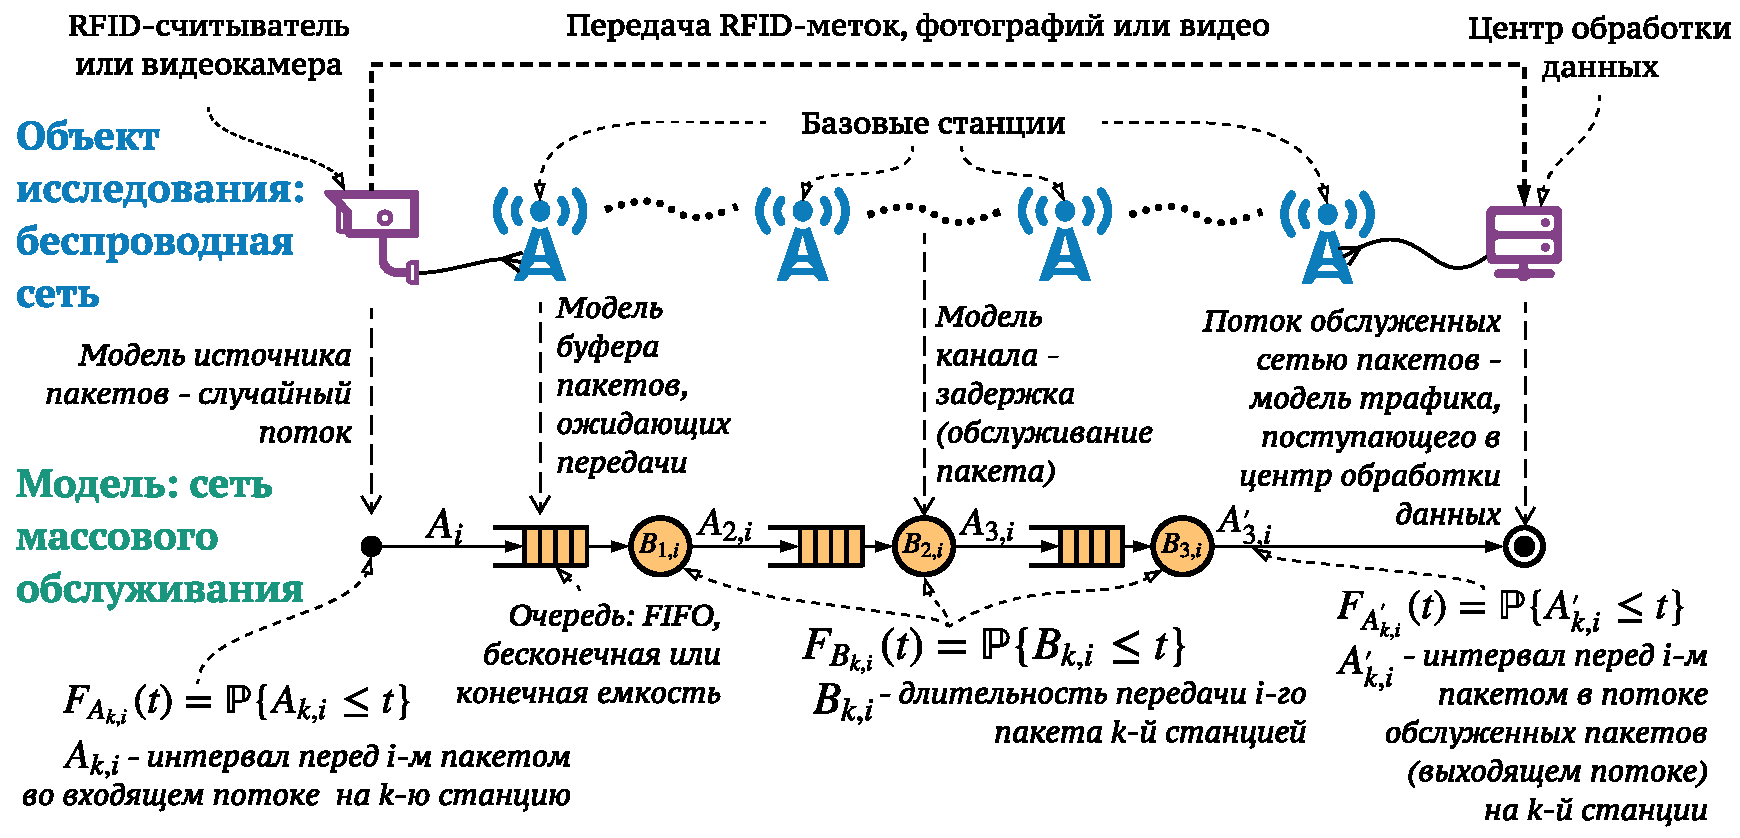
\includegraphics[width=1.0\textwidth]{chapter4/ch4_network_and_model}
  }
  \caption{Беспроводная сеть с линейной топологией и её аналитическая модель.}
  \label{fig:ch4_network_model}
\end{figure}

Для моделирования времени обслуживания будут использоваться PH-распределения $B_i \sim PH(S, \overline{\tau})$, а для моделирования интервалов между поступлениями в сеть пакетов "--- MAP-поток $A \sim MAP(D_0, D_1)$. Определения PH-распределений и MAP-потоков были даны в главе 1, а свойства, необходимые для вычисления характеристик тандемной сети массового обслуживания, будут приведены в следующем разделе.

Поставим формально задачу вычисления средней межконцевой задержки и вероятности потери пакетов из-за переполнения очередей в сети массового обслуживания. Пусть заданы длина сети (число узлов) $N$, емкость очередей $M$, входящий MAP-поток $X \sim MAP(D_0, D_1)$ и PH-распределения времени обслуживания $Y_k \sim PH(S_k, \overline{\tau}_k)$, $k = 1, 2, \dots, N$. Будем обозначать момент поступления $i$-го пакета на вход $k$-го узла как $t_{i,k}^{(a)}$, а момент завершения его обслуживания -- как $t_{i,k}^{(d)}$. Очевидно, что для любого $k < N$ выполняется $t_{i,k}^{(d)} = t_{i,{k+1}}^{(a)}$, если пакет не застает очередь $(k+1)$-го узла заполненной (в этом случае пакет теряется). Рассмотрим произвольный $i$-й пакет. Результатом обработки этого пакета может быть один из двух исходов: либо на некотором $k$-м узле пакет застанет очередь заполненной и будет отброшен, либо он будет обработан последовательно каждым из узлов, и покинет систему тогда, когда завершится его обработка последним узлом в момент $t_{i,N}^{(d)}$. Вероятность первого исхода (то есть потери пакета) будем обозначать $P_l$, она представляет собой долю пакетов, заставших какой-либо узел сети полностью заполненным. Для пакетов, которые не были потеряны, можно вычислить межконцевую задержку $\Delta t_i = t^{(d)}_{i,N} - t^{(a)}_{i,1}$.

Задача исследования состоит в поиске методов численной оценки средней межконцевой задержки $\overline{\Delta t}$ и вероятности потери пакета $P_l$.

Из-за экспоненциального роста размера пространства состояний при увеличении числа станций в сети, вычисление точных значений задержек и вероятностей потери пакетов возможно только для небольших сетей. Для получения оценок параметров в общем случае предлагается использовать метод редукции выходящих потоков, то есть заменять потоки обслуженных пакетов на выходе из очередного узла сети MAP-потоком небольшого размера. Этот метод будет подробно описан и численно исследован в этой главе диссертационной работы.

% На практике обычно известны только статистические оценки распределений или выборка интервалов между пакетами (например, полученная из сетевого дампа). Поэтому при выполнении численных экспериментов в качестве входных данных будем считать известными не сами матрицы $D_0, D_1, S, \overline{\tau}$, а моменты распределений. Пусть $m_a = \mathbb{E}X$ -- среднее время между поступлениями новых пакетов, $\sigma_a$ -- стандартное отклонение. Аналогично, пусть $m_s = \mathbb{E}Y$ -- среднее время обслуживания пакета, а $\sigma_s$ -- его стандартное отклонение. Время обслуживания будем задавать средним значением $m_s$, коэффициентом вариации $c_s = \sigma_s / m_s$ и коэффициентом асимметрии $\gamma_s = \mathbb{E}[(Y - m_s)^3] / \sigma_s^3$. Входящий поток будем задавать аналогично с помощью $m_a$, $c_a$ и $\gamma_a$, а также коэффициента автокорреляции между соседними интервалами $\rho_1$.


%%%%%%%%%%%%%%%%%%%%%%%%%%%%%%%%%%%%%%%%%%%%%%%%%%%%%%%%%%%%%%%%%%%%%%%%%%%%%%%%
\section{Открытая тандемная сеть массового обслуживания с узлами MAP/PH/1/M}\label{sec:ch4_queues}
%%%%%%%%%%%%%%%%%%%%%%%%%%%%%%%%%%%%%%%%%%%%%%%%%%%%%%%%%%%%%%%%%%%%%%%%%%%%%%%%

В этом разделе рассмотрим основные свойства PH-распределений, MAP-потоков и систем массового обслуживания MAP/PH/1/M. На базе этих свойств, сформулируем итерационный алгоритм, позволяющий рассчитывать характеристики сетей массового обслуживания типа MAP/PH/1/M $\rightarrow \bullet$/PH/1/M$\rightarrow \dots \rightarrow \bullet$/PH/1/M, и приведем анализ его сложности.


%%% ~~~~~~~~~~~~~~~~
\subsection{Свойства PH-распределений и MAP-потоков}\label{sec:ch4_queues_map_ph_props}
%%% ~~~~~~~~~~~~~~~~

Пусть $Y \sim PH(S, \overline{\tau})$, матрица $S$ и вектор $\overline{\tau}$ удовлетворяют ограничениям \eqref{eq:ch1_ph_def}. Тогда функция распределения $F(y)$ и моменты случайной величины $Y$ определяются как \cite{Buchholz2014}:

\begin{equation}
	\label{eq:ch4_ph_props}
	\begin{aligned}
		&F(y) = \mathbb{P}\{Y < y\} = 1 - \overline{\tau} e^{Sy} \mathbf{1}\\
		&\mathbb{E}Y^k = k! \overline{\tau} (-S)^{-k} \mathbf{1}
	\end{aligned}
\end{equation}

Пусть $X \sim MAP(D_0, D_1)$, где матрицы $D_0$ и $D_1$ удовлетворяют ограничениям \eqref{eq:ch1_map_def}. Матрица $D_1$ описывает переходы управляющей марковской цепи, сопровождающиеся генерацией пакетов (наблюдаемые переходы), а матрица $D_0$ "--- переходы, при которых генерации нового пакета не происходит (невидимые переходы). Если после генерации очередного пакета MAP-поток находится в состоянии $i$, время до появления следующего пакета имеет PH-распределние $X^{(i)} = PH(D_0, \overline{e}_i)$, где $\overline{e}_i = (0, \dots, 0, 1, 0, \dots, 0)$ "--- единичный вектор, в котором на $i$-й позиции стоит единица. Число состояний $W$ в управляющей цепи потока будем называть его размером или порядком и обозначать как $\vline X \vline$.

Функция распределения интервалов между событиями, значения моментов MAP-потока $X$ и коэффициенты корреляции с лагом $k$ определяются выражениям:

\begin{equation}
	\label{eq:ch4_map_props}
    \begin{aligned}
    \mathbb{P}\{X < t\} &= 1 - \overline{\alpha}e^{D_0 t}\overline{\mathbf{1}}\\
    \mathbb{E}X^{k} &= k! \overline{\alpha}(-D_0)^{-k}\overline{\mathbf{1}}\\
    \rho_k &= \frac{\lambda \overline{\pi} P^k (-D_0)^{-1} \overline{\mathbf{1}} - 1}{2 \overline{\pi} (-D_0)^{-1} \overline{\mathbf{1}} - 1}.
    \end{aligned}
\end{equation}
Здесь $P = (-D_0)^{-1} D_1$ "--- матрица вложенной цепи. Эта матрица $P$ и вектор стационарных вероятностей $\overline{\alpha}$ рассчитываются с помощью системы линейных алгебраических уравнений:

\begin{equation}
\label{eq:ch4_map_dtmc}
	\overline{\alpha}: \begin{cases}
		\overline{\alpha} P = \overline{\alpha} \\
		\sum\limits_{i=1}^{W} \alpha_i = 1
 	\end{cases}
\end{equation}

Стационарное распределение $\overline{\pi} \in \mathbb{R}^W$ вероятностей потока $MAP(D_0, D_1)$ является решением системы линейных уравнений:

\begin{equation}
	\label{eq:ch4_map_pmf}
	\begin{cases}
		\overline{\pi}(D_0 + D_1) &= \overline{\mathbf{0}}\\
		\overline{\pi}\overline{\mathbf{1}} &= 1
	\end{cases},
\end{equation}
где $\overline{\mathbf{0}}$ и $\overline{\mathbf{1}}$ "--- вектор-строки, состоящие из всех нулей и единиц соответственно.

Интенсивность MAP-потока можно найти как $\lambda = (\mathbb{E}X)^{-1}$. Её можно вычислить как математическое ожидание случайной величины, равной суммарной интенсивности наблюдаемых переходов:

\begin{equation}
	\label{eq:ch4_map_rate}
	\lambda = \sum\limits_{j=1}^{W} \pi_j \sum\limits_{k=1}^{W} \{D_1\}_{jk} = \overline{\pi} D_1 \overline{\mathbf{1}}
\end{equation}
Формула (\ref{eq:ch4_map_rate})~удобна, когда не требуется вычисление моментов старших порядков или коэффициентов автокорреляции, т.к. в этом случае также не требуется обращать матрицу $D_0$.

\begin{figure}[h]
    \centerfloat{
      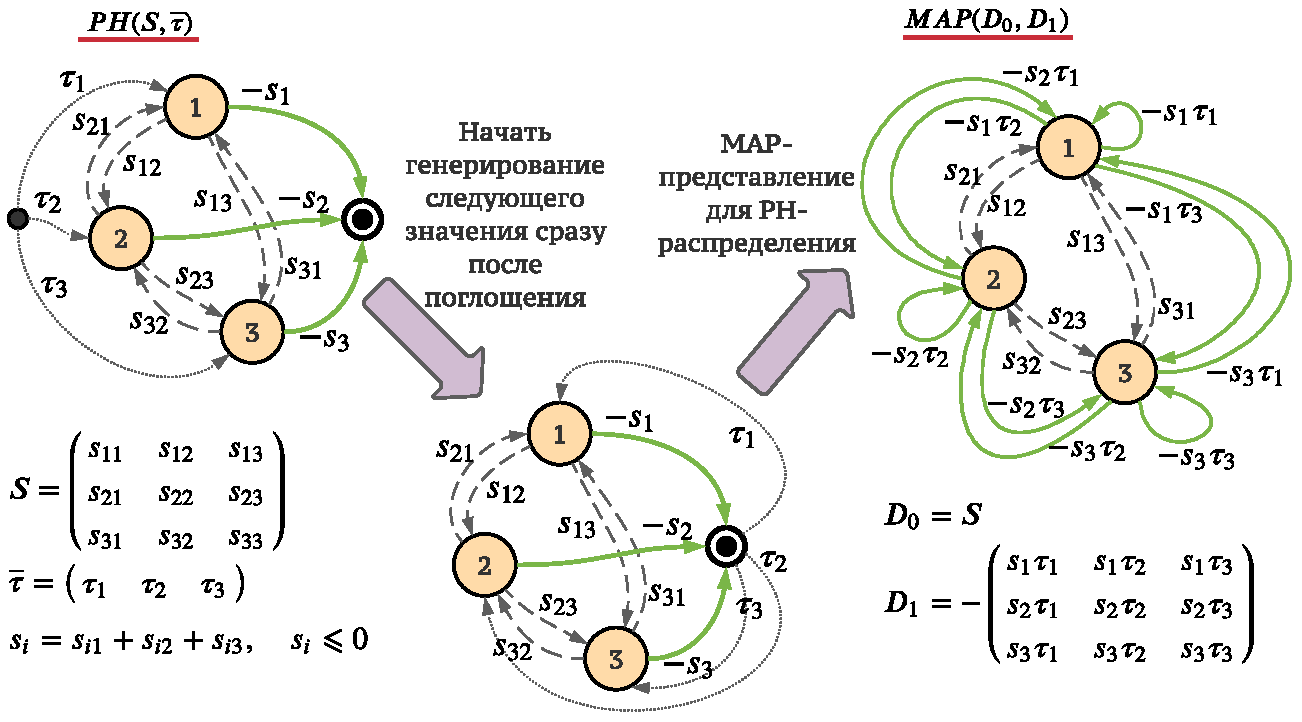
\includegraphics[width=1.0\textwidth]{chapter4/ch4_ph2map}
    }
    \caption{Пример построения MAP-потока, в котором все интервалы имеют одинаковое PH-распределение $PH(S, \overline{\tau})$ с тремя состояниями управляющей цепи.
    \label{fig:ch4_ph2map}}
\end{figure}

MAP-поток является обобщением над PH-распределением. Существенной чертой MAP-потока является то, что корреляция между интервалами может быть отличной от нуля (см. формулу~\eqref{eq:ch4_map_props}). В то же время, последовательность интервалов, каждый из которых имеет PH-распределение с одинаковыми параметрами $PH(S, \overline{\tau})$, также можно считать MAP-потоком, автокорреляция в котором будет нулевой. Для PH-распределения $PH(S, \overline{\tau})$ соответствующий MAP-поток будет иметь матрицы следующего вида:

\begin{equation}
    \label{eq:ch4_map_ph_representation}
    D_0 = S, \qquad D_1 = (-S \overline{1}) \overline{\tau} = -\left(
        \begin{matrix}
            s_1\\
            s_2\\
            \vdots\\
            s_V
        \end{matrix}
     \right) \left(
         \begin{matrix}
            \tau_1 & \tau_2 & \dots &
         \end{matrix}
     \right),
\end{equation}
где $s_i = \sum_{j=1}^V s_{ij}$
Пример построения MAP-потока по PH-распределению приведен на рис.~\ref{fig:ch4_ph2map}.



%%% ~~~~~~~~~~~~~~~~
\subsection{Свойства системы MAP/PH/1/M}\label{sec:ch4_queue_net_system_props}
%%% ~~~~~~~~~~~~~~~~

Ключевое свойство систем массового обслуживания MAP/PH/1/M, благодаря которому их удобно использовать для моделирования многошаговых сетей -- замкнутость на множестве MAP-потоков: согласно следующим теоремам (см. \cite{VishnevskyDudin2018}), результат просеивания MAP-потока "--- MAP-поток, сумма MAP-потоков "--- MAP-поток, и поток обслуженных заявок, выходящих из системы MAP/PH/1/M, также является также MAP-потоком. В дальнейшем будем обозначать выходной поток $Z$ из системы массового обслуживания с входным потоком $X$, временем обслуживания $Y$ и емкостью очереди $M$ как $\mathcal{D}(X, Y, M)$.

\begin{thm}\label{th:ch4_sifted_map}\textnormal{\cite{VishnevskyDudin2018}}
  Результат просеивания MAP-потока $X \sim MAP(D_{0},D_{1})$ с вероятностью $p$ "--- MAP-поток $X_{p} \sim MAP(D_{0}+(1-p)D_{1},pD_{1})$ (в дальнейшем обозначается как $pX$)
\end{thm}

\begin{thm}\label{th:ch4_maps_sum}\textnormal{\cite{VishnevskyDudin2018}}
  Сумма MAP-потоков $X_{1}$ и $X_{2}$, $X_i \sim MAP(D_{0}^{(i)},D_{1}^{(i)})$, $i=1,2$ "--- MAP-поток $X$:
  $$
    X = X_{1} \oplus X_{2} \sim MAP(D_{0}^{(1)} \oplus D_{0}^{(2)},D_{1}^{(1)} \oplus D_{1}^{(2)}),
  $$
  где $\oplus$ "--- сумма Кронекера.
\end{thm}

\textbf{Замечание.} Если потоки $X_1$ и $X_2$ имеют размерности $W_1$ и $W_2$, то размерность суммарного потока $X$ равняется $W = W_1 W_2$.

\begin{thm}\label{th:ch4_map_departure}\textnormal{\cite{VishnevskyDudin2018}}
    Пусть в системе MAP/PH/1/M $X \sim MAP(D_{0}$ $D_{1})$, $D_i \in \mathbb{R}^{W \times W}, i=0,1$ -- входящий поток, $Y \sim PH(S, \overline{\tau})$, $\mathbb{R}^{V \times V}$ -- время обслуживания, обслуживание ведется согласно дисциплине FIFO, а ёмкость очереди равна $M$. Тогда поток выходящих (обслуженных) пакетов есть MAP-поток $Z \sim MAP(D'_{0},D'_{1})$, матрицы которого определяются как:
    \begin{equation}
        \label{eq:ch4_qs_departure_d0}
        D'_{0} =
        \begin{bmatrix}
            D_{0} \otimes I_{V} & D_{1}\otimes (\overline{\tau} \otimes \overline{\mathbf{1}}_{V}) & 0 & \cdots & 0 & 0\\
            0 & D_{0} \otimes S & D_{1} \otimes I_{V} & \cdots & 0 & 0\\
            0 & 0 & D_{0} \otimes S & \cdots & 0 & 0 \\
            \vdots & \vdots & \vdots & \ddots & \vdots & \vdots \\
            0 & 0 & 0 & \cdots & D_{0} \otimes S & D_{1} \otimes I_{V}\\
            0 & 0 & 0 & \cdots & 0 & (D_{0}+D_{1}) \otimes S
        \end{bmatrix},
    \end{equation}
    \begin{equation}
        \label{eq:ch4_qs_departure_d1}
        D'_{1} =
          \begin{bmatrix}
              0 & \cdots & 0 & 0 \\
              I_{W} \otimes C_{t} & \cdots & 0 & 0 \\
              \vdots & \ddots & \vdots & \vdots \\
              0 & \cdots & 0 & I_{W} \otimes C_{t} & 0
          \end{bmatrix},
    \end{equation}
    где $C_{t} = (-S \overline{\mathbf{1}}_{V}) \otimes \overline{\tau}$, а $I_V$, $I_W$ -- едининые матрицы порядка $V$ и $W$ соответственно.
\end{thm}

Из структуры матриц потока $Z$ можно сделать следующие выводы. Во-первых, поток $Z$ имеет размерность $|Z| = (M+2)|X| |Y| = (M+2) V W$. Во-вторых, каждому состоянию потока $Z$ соответствует некоторое число пакетов в системе и состояния входящего MAP-потока $X$ и обслуживающего прибора $Y$. Пусть управляющая цепь потока $Z$ находится в состоянии $n$. Тогда в системе $\lfloor \frac{n}{VW} \rfloor$ пакетов, входящий MAP-поток находится в состоянии $\lfloor \frac{n (\mathbf{mod}\;VW)}{V} \rfloor + 1$, а обслуживающий прибор -- в состоянии $n(\mathbf{mod} V)+1$.

Предыдущее замечание можно обощить. По сути, при построении матриц выходящего MAP-потока производится построение марковской цепи, управляющей работой системы MAP/PH/1/M. Действительно, в такой системе переходы происходят из-за возникновения одного из двух событий: переход в цепи входящего MAP-потока или переход в цепи PH-распределения. При этом, если переход в цепи входящего потока сопровождается формированием сообщения, и система не находится в состоянии полностью заполненной очереди, то размер системы увеличивается. Если же переход происходит в цепи PH-распределения в поглощающее состояние, то размер системы уменьшается на единцицу. Элементы матрицы $D'_0$ соответствуют всем переходам, кроме поглощения в цепи PH-распределения, последним же соответствуют элементы матрицы $D'_1$. По этой причине, когда будет требоваться найти распределение вероятностей управляющей цепи системы MAP/PH/1/M, будем использовать инфинитезимальый генератор управляющей цепи выходящего потока $Z$.

Обозначим $\overline{\pi}$ стационарное распределение $X$, а $\overline{\theta}$ стационарное распределение $Z$. Вектор $\overline{\theta}$ можно переписать в виде $\overline{\theta} = (\overline{\theta}_0, \overline{\theta}_1, \dots, \overline{\theta}_{M+1})$, где $\overline{\theta}_k$ "--- часть вектора $\overline{\theta}$, соответствующая тем состояниям системы, в которых число пакетов равно $k$. Пусть $\mu(t)$ "--- случайный процесс, значение которого в каждый момент времени равняется числу пакетов в системе. Обозначим $p_k = \lim\limits_{t \rightarrow \infty} \mathbb{P}\{\mu(t) = k\}$ "--- стационарная вероятность того, что в системе $k=\overline{0,M+1}$ пакетов. Тогда, зная стационарное распределение $\overline{\theta}$ управляющей цепи MAP-потока $Z$, можно вычислить распределение $\overline{p}$:

\begin{equation}
	\label{eq:ch4_qs_size_pmf}
	p_k = \sum\limits_{j=1}^{VW} \{ \overline{\theta}_k \}_j.
\end{equation}
Отсюда можно рассчитать среднее число пакетов в системе как $m_1 = \mathbb{E}\mu$:

\begin{equation}
  \label{eq:ch4_qs_size_avg}
  \begin{aligned}
	  m_1 = \sum\limits_{k=0}^{M+1} k \mathbb{P}\{\mu = k\} = \sum\limits_{k=0}^{M+1} k p_k = \sum\limits_{k=0}^{M+1} k \sum\limits_{j=1}^{VW} \{ \overline{\theta}_k \}_j = \sum\limits_{k=0}^{M+1} \sum\limits_{j=1}^{VW} k \theta_{kVW+j}\hfill.
  \end{aligned}
\end{equation}

Для получения вероятности потери пакета из-за переполнения очереди нужно более подробно рассмотреть часть вектора $\overline{\theta}$, соответствующую случаю заполненной очереди (т.е. $\mu=M+1$). Состояния внутри блоков матриц \eqref{eq:ch4_qs_departure_d0} и \eqref{eq:ch4_qs_departure_d1} сгруппированы по состояниям входящего MAP-потока, т.е. состояния $\{ \overline{\theta}_k \}_{jV + 1}, \dots \{ \overline{\theta}_k \}_{(j+1)V}$ соответствуют всевозможным состояниям цепи PH-распределения и состоянию $j$ входящего MAP-потока, когда в системе $k$ пакетов. Определим:

\begin{equation}
    \label{eq:ch4_qs_size_slice_pmf}
    \overline{\psi}_k = ( \sum\limits_{j=1}^{V}\{ \overline{\theta}_k \}_j, \dots, \sum\limits_{j=1}^{V}\{ \overline{\theta}_{k} \}_{(W-1)V + j} )
\end{equation}
"--- распределение вероятностей входящего MAP-потока при $k$ пакетах в системе. Тогда вероятность $P_L$ потери пакета можно выразить так:

\begin{equation}
  \label{eq:ch4_qs_loss_prob}
  P_L = \overline{\psi}_{M+1} \frac{D_1}{\lambda_X}\overline{\mathbf{1}}
\end{equation}

Наконец, зная интенсивность входящего потока $\lambda_{X}$, среднее число пакетов в системе $m_1$ и вероятность потери пакетов $P_L$, используя формулу Литтла, можно рассчитать среднюю задержку:

\begin{equation}
	\label{eq:ch4_qs_delay}
	T = \frac{m_1}{(1 - P_L)\lambda_{X}}.
\end{equation}
Множитель $(1 - P_L)$ в знаменателе возникает в следствие того, что из-за переполнения очереди лишь часть пакетов входящего потока попадает в систему, т.е. фактическая интенсивность потока пакетов, поступающих в систему, составляет $(1 - P_L) \lambda_{X}$.



%%% ~~~~~~~~~~~~~~~~
\subsection{Точный расчёт характеристик сети массового обслуживания}\label{sec:ch4_queue_net_precise}
%%% ~~~~~~~~~~~~~~~~


Используя формулы \eqref{eq:ch4_qs_size_avg}, \eqref{eq:ch4_qs_loss_prob} и \eqref{eq:ch4_qs_delay} несложно вычислить среднюю межконцевую задержку пакетов в сети и вероятность потери пакета на каком либо узле. Будем рассматривать два варианта сетей: сети с кросс-трафиком, в которых потоки данных поступают на каждый узел, и сети без кросс-трафика, в которых внешний трафик поступает только на первую станцию, и все последующие станции передают только его.

\begin{figure}[htb]
	\centerfloat{
    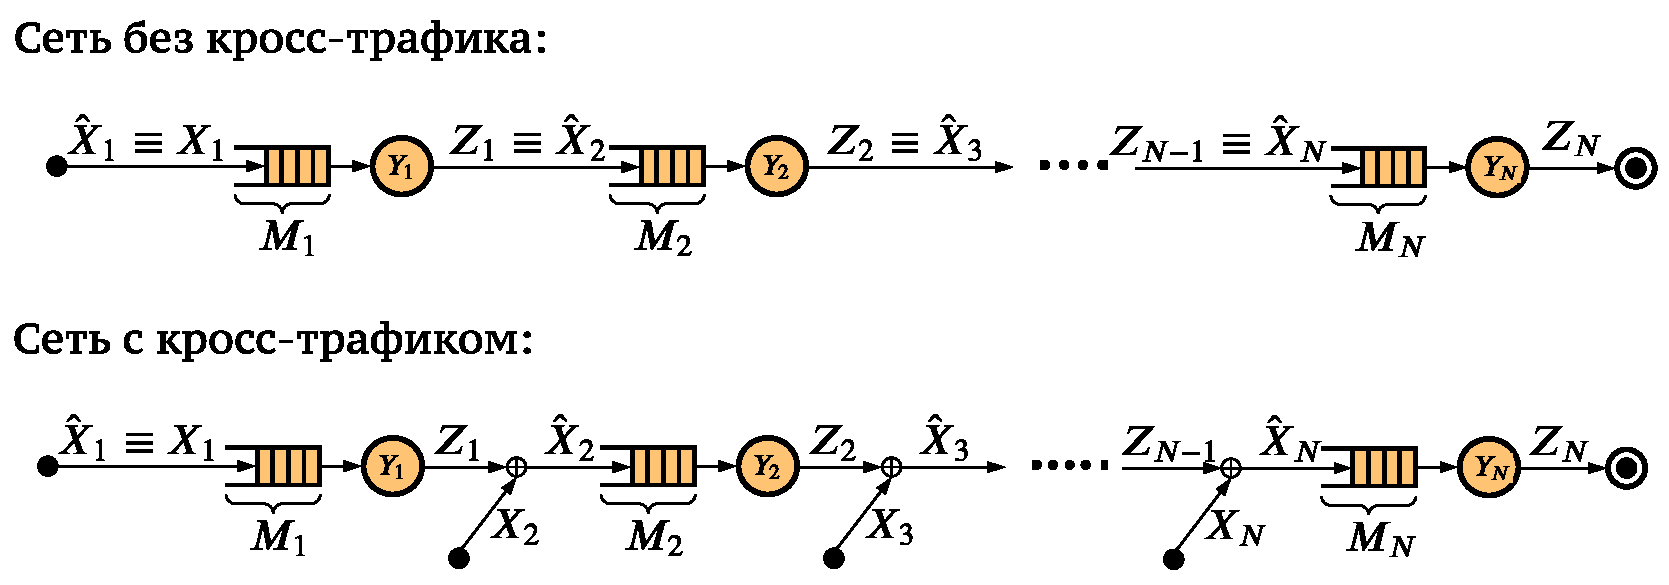
\includegraphics[width=0.95\textwidth]{chapter4/ch4_queueing_networks}
  }
  \caption{Сети массового обслуживания с кросс-трафиком и без него.}
  \label{fig:ch4_queueing_networks}
\end{figure}

Пусть в сети (см. рис. \ref{fig:ch4_queueing_networks}) $N$ станций, емкость очереди на $i$-й станции ($i = 1,2, \dots, N$) равна $M_i \in \mathbb{N}$, а длительность обслуживания $Y_i$ имеет PH-распределение $Y_i \sim PH(S_i, \overline{\tau})$, $S_i \in \mathbb{R}^{V_i \times V_i}$, $V_i \in \mathbb{N}$. Если в сети есть кросс-трафик, то на каждую станцию поступает пользовательский поток $X_i \sim MAP(D_{0,i}, D_{1,i})$; если кросс-трафика нет, то поток $X_1 \equiv X = MAP(D_0, D_1)$ поступает только на первую станцию. Обозначим порядок входящего MAP-потока на $i$-ю станцию как $W_i$, то есть $D_{0,i}, D_{1,i} \in \mathbb{R}^{W_i \times W_i}$, $W_i \in \mathbb{N}$.

Обозначим $Z_i$ - выходящий MAP-поток с $i$-й станции, а $\hat{X}_i$ - общий входящий поток на $i$-ю станцию. Тогда, согласно теоремам \ref{th:ch4_maps_sum} и \ref{th:ch4_map_departure}, потоки $\hat{X}_i$ и $Z_i$ "--- MAP-потоки. Используя ранее введённые обозначения, их можно определить формально следующим образом:

\begin{equation}
  \label{eq:ch4_total_arrival_and_departure}
  \begin{aligned}
    \hat{X}_1 &\equiv X_1\\
    \hat{X}_i &= \begin{cases}
      X_i \oplus Z_{i-1},&\text{в сети есть кросс-трафик и } i = 2,3, \dots, N\\
      Z_{i-1},&\text{в сети нет кросс-трафика}
    \end{cases}\\
    Z_i &= \mathcal{D}(\hat{X}_i, Y_i, M)
  \end{aligned}
\end{equation}

Обозначим порядок выходящих MAP-потоков $Z_i$ как $U_i$, $i=1,2,\dots N$, то есть $Z_i \sim MAP(\tilde{D}_{i,0}, \tilde{D}_{i,1})$ и $\tilde{D}_{i,0}, \tilde{D}_{i,1} \in \mathbb{R}^{U_i \times U_i}$. Тогда величина $U_i$ определяется с помощью следующего утверждения.

\begin{prop}\label{prop:ch4_departure_order}
	Порядок $U_i$ MAP-потока обслуженных пакетов $Z_i$ на выходе из $i$-го узла, $i = 1,2,\dots N$, определяется как:
	$$
	U_i = \begin{cases}
		\prod\limits_{j=1}^{i}(M_j + 2)V_jW_j,&\text{если в сети есть кросс-трафик}\\
		W_1\prod\limits_{j=1}^{i}(M_j + 2)V_j,&\text{если кросс-трафика нет}.
	\end{cases}
	$$
\end{prop}
\begin{proof}
Утверждение доказывается по индукции. При $i = 1$ $Z_1 = \mathcal{D}(X_1, Y_1, M_1)$ и $U_1 = (M_1 + 2)V_1W_1$ согласно замечанию к теореме \ref{th:ch4_map_departure}.

Пусть утверждение верно при $i = n-1$. Если в сети нет кросс-трафика, то $Z_i = \mathcal{D}(\hat{X}_i, Y_i, M_i) = \mathcal{D}(Z_{i-1}, Y_i, M_i)$ и величина $U_i$ определяется как:
$$
  \begin{aligned}
    U_i &= (M_i + 2) V_i U_{i-1} = (M_i + 2) V_i \times (W_1 \prod\limits_{j=1}^{i-1}(M_j + 2)V_j)\\
    &= W_1 \prod\limits_{j=1}^{i}(M_j + 2)V_j.
  \end{aligned}
$$
Если же в сети есть кросс-трафик, то
$$
  Z_i = \mathcal{D}(\hat{X}_i, Y_i, M_i) = \mathcal{D}(Z_{i-1} \oplus X_i, Y_i, M_i),
$$
и порядок потока $Z_i$ определяется следующей цепочкой равенств:
$$
  \begin{aligned}
    U_i &= (M_i + 2) V_i (U_{i-1} W_i) = (M_i + 2) V_i W_i \times \prod\limits_{j=1}^{i-1}(M_j + 2) V_j W_j)\\
    &= \prod\limits_{j=1}^{i}(M_j + 2) V_j W_j.
  \end{aligned}
$$
\end{proof}

Схема расчёта характеристик сети выглядит следующим образом.

\textit{Шаг 1.} Положим $i := 1$.

\textit{Шаг 2.} Если $i = 1$, то положим $\hat{X}_i = X_1$. Если же $i > 1$, то вычисляем $\hat{X}_i$ согласно \eqref{eq:ch4_total_arrival_and_departure}: $\hat{X}_i = Z_{i-1}$, если в сети нет кросс-трафика, и $\hat{X}_i = Z_{i-1} \oplus X_i$ иначе. Обозначим матрицы потока $\hat{X}_i$ как $\hat{D}_{i,0}$ и $\hat{D}_{i,1}$, то есть $\hat{X}_i = MAP(\hat{D}_{i,0}, \hat{D}_{i,1})$.

\textit{Шаг 3.} С помощью теоремы \ref{th:ch4_map_departure} вычисляем матрицы $D'_{i,0}$, $D'_{i,1}$ MAP-потока $Z_i = \mathcal{D}(\hat{X}_i, Y_i, M_i)$.

\textit{Шаг 4.} Для выходящего MAP-потока $Z_i$ вычисляем его стационарное распределение $\overline{\theta}^{(i)}$ с помощью системы линейных алгебраических уравнений:
$$
  \begin{cases}
	  \overline{\theta}^{(i)}(D'_{i,0} + D'_{i,1}) &= 0\\
	  \overline{\theta}^{(i)} \mathbf{1} &= 1
  \end{cases}
$$

\textit{Шаг 5.} Рассчитываем среднее число пакетов в очереди $i$-й станции согласно \eqref{eq:ch4_qs_size_avg}:
$$
  m_1^{(i)} = \sum\limits_{k=0}^{M_i + 1} k \sum\limits_{j=1}^{V_i \hat{W}_i} \theta^{(i)}_{k V_i \hat{W}_i + j}\;,
$$
где $V_i = |Y_i|$ "--- порядок PH-распределения $Y_i$, а $\hat{W}_i = |\hat{X}_i|$ "--- порядок входящего MAP-потока $\hat{X}_i$.

\textit{Шаг 6.} Определяем стационарное распределение вероятностей $\overline{\pi}^{(i)}$ входящего потока $\hat{X}_i$. Если в сети нет кросс-трафика и $i > 1$, то полагаем $\overline{\pi}^{(i)} \equiv \overline{\theta}^{(i-1)}$. В противном случае находим $\overline{\pi}^{(i)}$ как решение системы линейных алгебраических уравнений:
$$
  \begin{cases}
	  \overline{\pi}^{(i)}(\hat{D}_{i,0} + \hat{D}_{i,1}) &= 0\\
	  \overline{\pi}^{(i)} \mathbf{1} &= 1
  \end{cases}
$$

\textit{Шаг 7.} С помощью найденного на предыдущем шаге стационарного распределения $\overline{\pi}^{(i)}$ входящего потока $\hat{X}_i$ и формулы \eqref{eq:ch4_map_rate} вычисляем интенсивность поступления пакетов на $i$-ю станцию:
$$
  \lambda_i = \overline{\pi}^{(i)} \hat{D}_{i,1} \overline{\mathbf{1}}.
$$

\textit{Шаг 8.} Рассчитываем распределение состояний входящего MAP-потока при наличии в системе $M_i + 1$ пакета (то есть при заполненной системе):
$$
  \overline{\psi}^{(i)} = \left(
  \sum\limits_{j=1}^{V_i} \{ \overline{\theta}^{(i)}_{M_i+1} \}_j,
  \dots,
  \sum\limits_{j=1}^{V_i} \{ \overline{\theta}^{(i)}_{M_i+1} \}_{(\hat{W}_i-1) V_i + j}
  \right).
$$
Здесь вектор $\overline{\theta}_{M_i+1}^{(i)}$ "--- часть вектора $\overline{\theta}^{(i)}$, относящаяся к состояниям системы, когда в ней находится $M_i + 1$ пакет.

\textit{Шаг 9.} Вычисляем векроятность потери пакета из-за переполнения $i$-й очереди с помощью~\eqref{eq:ch4_qs_loss_prob}:
$$
  P_L^{(i)} = \overline{\psi}^{(i)} \frac{\hat{D}_{i,0}}{\lambda_i} \overline{\mathbf{1}}.
$$

\textit{Шаг 10.} Вычисляем среднюю задержку пакетов на $i$-й станции с помощью~\eqref{eq:ch4_qs_delay}:
$$
  T_i = \frac{m_1^{(i)}}{(1 - P_L^{(i)}) \lambda_i}
$$

\textit{Шаг 11.} Если $i < N$, то увеличиваем $i := i + 1$ и переходим на шаг 2. В противном случае переходим далее, на шаг 12.

\textit{Шаг 12.} Вычисляем вероятность потери пакета $P_L = \prod\limits_{i=1}^{N} (1 - P_L^{(i)})$.

\textit{Шаг 13.} Вычисляем общую задержку $T = \sum\limits_{i=1}^{N} T_i$.

Предложенная схема проста в вычислении. По сути, на каждом шаге с помощью нескольких операций произведения Кронекера строятся блочные матрицы для выходящего MAP-потока, а также, если в сети есть кросс-трафик, с помощью суммы Кронекера строятся матрицы входящего потока. Далее решаются две (если в сети есть кросс-трафик) или одна (в противном случае) системы линейных алгебраических уравнений для определения стационарных вероятностей входящего и исходящего потока. Наконец, с помощью нескольких операций умножений найденных распределений на матрицы потоков, вычисляются искомые характеристики "--- вероятность потери пакета, средний размер системы и задержка.

Главный недостаток этой схемы расчета "--- чрезвычайно высокая вычислительная сложность.

\begin{prop}\label{prop:ch4_base_algorithm_complexity}
  Пусть входящие MAP-потоки имеют порядок $W$, PH-распределения "--- порядок $V$, ёмкость очередей равна $M$, и сеть содержит $N$ станций. Тогда итерационная схема расчета характеристик тандемной сети имеет сложность:
  \begin{itemize}
	  \item $O((M V W)^{3N})$, если в сети есть кросс-трафик
	  \item $O(W^3 (M V)^{3N})$, если кросс-тррафика в сети нет.
  \end{itemize}
\end{prop}
\begin{proof}
Рассмотрим $i$-ю итерацию алгоритма, $i \leqslant N$, то есть расчёт характеристик $i$-й станции сети. Отметим сперва, что при $i > 1$ порядок выходящего потока с предыдущей $i-1$-й станции есть $(M + 2) V \hat{W}_i$, где $\hat{W}_i$ "--- порядок входящего потока на $i$-ю станцию. Согласно \ref{prop:ch4_departure_order}, при наличии в сети кросс трафика $U_i = ((M+2)VW)^i$, а если кросс-трафика нет, то $U_i = W((M+2)V)^i$.

Сложность итерации определяется шагами 4 и 6, в которых необходимо решать системы линейных алгебраических уравнений, причем порядок матрицы системы на шаге 4 (генератор выходящего потока) заведомо выше, чем системы на шаге 6 (генератор входящего потока). Полагая, что для решения системы используется алгоритм наподобии метода Гаусса, на шаге 4 потребуется $O(U_i^3)$ операций. Остальные шаги имеют более низкую сложность: шаги 1, 10 и 11 "--- $O(1)$, шаг 2 "--- $O(U_{i-1}^2 W^2)$, шаг 3 "--- $O(U_i^2)$, шаг 5 "--- $O(VW + M)$, шаги 7 и 9 "--- $O(U_i^2)$, шаг 8 "--- $O(VM)$. Сложность шагов 12 и 13 есть $O(N)$.

Таким образом, если в сети есть кросс-трафик, сложность алгоритма составит
$$
  \begin{aligned}
    O((VWM)^3) &+ O((VWM)^6) + \dots + O((VWM)^{3N}) + O(N) \\
    &= O(VWM)^{3N},
  \end{aligned}
$$
а если кросс-трафика в сети нет, то
$$
  \begin{aligned}
    O(W^3 (VM)^3) &+ O(W^3 (VM)^6) + \dots + O(W^3 (VM)^{3N}) + O(N) \\
    &= O(W^3 (VM)^{3N}).
  \end{aligned}
$$

\end{proof}

\textbf{Замечание 1.} Учитывая, что матрицы выходящего потока $Z_i$ имеют блочный трехдиагональный вид, они будут сильно разрежены. Благодаря этому можно попытаться применить более эффективные способы решения системы алгебраических уравнений. Однако, показатель степени в оценке сложности все равно не окажется ниже, чем $(2 + \epsilon) N$.


На практике утверждения \ref{prop:ch4_departure_order} и \ref{prop:ch4_base_algorithm_complexity} означают, что искать решения с помощью представленной схемы вычислений становится невозможным даже при относительно небольших $N$, $V$ и $W$. В таблице \ref{table:ch4_map_order_growth} приведены примеры роста порядков для различных порядков входящих процессов и времен обслуживания.

\begin{table}[h!]
\centering
\begin{tabular}{ |c|c|c||c|c|c|c|c| }
\hline
\multicolumn{3}{|c||}{} & \multicolumn{5}{c|}{Номер станции} \\
\hline
%\multirow{2}{4em}{Сеть без кросс-трафика, число станций}\\
$W$ & $V$ & $M$ & 1 & 2 & 3 & 4 & 5\\
\hline
\multicolumn{8}{|c|}{Сети без кросс-трафика} \\
\hline
1 & 1 & 1 & 3 & 9 & 27 & 81 & 243 \\
1 & 1 & 3 & 5 & 25 & 125 & 625 & 3'125 \\
2 & 2 & 2 & 16 & 128 & 1'024 & 8'192 & 65'536 \\
3 & 1 & 3 & 15 & 75 & 375 & 1'875 & 9'375 \\
1 & 3 & 3 & 15 & 225 & 3'375 & 50'625 & 759'375 \\
3 & 3 & 3 & 45 & 675 & 10'125 & 151'875 & 2'278'125 \\
\hline
\multicolumn{8}{|c|}{Сети с кросс-трафиком} \\
\hline
1 & 1 & 1 & 3 & 9 & 27 & 81 & 243 \\
1 & 1 & 3 & 5 & 25 & 125 & 625 & 3'125 \\
2 & 2 & 2 & 16 & 256 & 4'096 & 65'536 & 1'048'576 \\
3 & 1 & 3 & 15 & 225 & 3'375 & 50'625 & 759'375 \\
1 & 3 & 3 & 15 & 225 & 3'375 & 50'625 & 759'375 \\
3 & 3 & 3 & 45 & 2'025 & 91'125 & 4'100'625 & 184'528'125 \\
\hline
\end{tabular}
\caption{Порядки выходящих MAP-потоков в зависимости от порядков PH-распределения ($V$), входящих MAP-потоков ($W$) и ёмкости очереди ($M$).\label{table:ch4_map_order_growth}
}
\end{table}

Таким образом, для практического применения открытых сетей с узлами MAP/PH/1/M необходимы более эффективные методы расчета, пусть даже их результаты будут приближенными.




%%%%%%%%%%%%%%%%%%%%%%%%%%%%%%%%%%%%%%%%%%%%%%%%%%%%%%%%%%%%%%%%%%%%%%%%%%%%%%%%
\section{Расчёт характеристик сети массового обслуживания методом Монте-Карло}
%%%%%%%%%%%%%%%%%%%%%%%%%%%%%%%%%%%%%%%%%%%%%%%%%%%%%%%%%%%%%%%%%%%%%%%%%%%%%%%%

Расчёт методом Монте-Карло заключается в многократном проигрывании прохождения пакетов по сети массового обслуживания и замерах длительностей их пребывания в узлах, длин очередей и потерь. Для реализации этого метода лучше всего подходят системы дискретно-событийного моделирования, в которых обрабатываются возникающие события, а время изменяется только в начале обработки очередного события.

Методы и алгоритмы имитационного моделирования открытых сетей массового обслуживания хорошо известны, поэтому далее приведем лишь краткое схематичное описание работы модели и способа расчёта характеристик сети.

Для моделирования сети с узлами MAP/PH/1/M нужно описать обработку двух типов событий: появление нового пакета во входящем MAP-потоке и завершение обработки пакета на узле.

Пусть, как и ранее, $N$ "--- число станций в сети. Обозначим $K$ "--- глобальный счетчик пакетов, $T_k^a$ "--- время появления $k$-го пакета, $\Delta$ "--- множество вычисленных задержек, $a_i$ "--- число сгенерированных пакетов из $i$-го потока, $l_i$ "--- число потерянных пакетов на $i$-й станции, $t$ "--- модельное время, $n_i$ "--- число пакетов на $i$-й станции.

Если какая-либо из перечисленных величин $\chi$ будет нас интересовать в определенный момент модельного времени $t$, то будем писать $\chi(t)$. Кроме того, при описании операций будем использовать запись $\chi' := f(\chi)$, подразумевая, что после завершения выполнения текущего действия величина $\chi$ примет значение $\chi'$, а до окончания операции она сохраняет значение $\chi$.


%%% ~~~~~~~~~~~~~~~~
\subsection{Обработка событий}
%%% ~~~~~~~~~~~~~~~~

При \textbf{инициализации} модели для каждого потока $X_i$ выбирается интервал до поступления первого пакета $\tau_i$, и на время $\tau_i$ назначается обработка события поступления пакета на $i$-ю станцию.

Рассмотрим действия, происходящие при возникновении событий поступления нового пакета и завершении обслуживания.

\textbf{Обработка поступления нового пакета.} Если в момент времени $t = t_0$ во входящем потоке, поступающем в узел с номером $i$, происходит появление пакета, выполняются следующие действия.

\textit{Шаг 1.} Пакет обрабатывается в зависимости от того, занят ли прибор и есть ли место в очереди:
\begin{itemize}
  \item Если $n_i = 0$, то есть обслуживающий прибор узла $i$ свободен, то вычисляется случайная длительность обслуживания $\tau_s$, $\mathbb{P}\{\tau_s \leqslant \tau\} = F_{Y_i}(\tau)$, на момент времени $t_0 + \tau_s$ назначается событие окончания обслуживания на $i$-м приборе, а число пакетов в системе увличивается на единицу: $n'_i := n_i + 1$.
  \item Если $1 \leqslant n_i \leqslant M_i$, то есть обслуживающий прибор занят, но в очереди есть место, то пакет помещается в очередь, и счётчик числа пакетов в системе увличивается на единицу: $n'_i := n_i + 1$.
  \item Если $n_i = M_i + 1$, то есть в очереди нет места, пакет теряется, а счётчик потерянных пакетов $l_i$ увеличивается на единицу: $l'_i := l_i + 1$.
\end{itemize}

\textit{Шаг 2.} Для пакета сохраняется время его появления $T_K^a := t_0$.
\textit{Шаг 3.} Счётчики числа сгенерированных пакетов $K$ и $a_i$ увеличиваются на единицу: $K' := K + 1$, $a'_i := a_i + 1$.
\textit{Шаг 4.} Выбирается случайное время до следующего появления пакета в $i$-м потоке $\tau_a$, $\mathbb{P}\{ \tau_a \leqslant \tau \} = F_{X_i}(\tau)$, на момент $t_0 + \tau_a$ назначается следующее событие появления нового пакета в $i$-м потоке.

\textbf{Завершение обслуживания пакета.} Если в момент времени $t_0$ завершается обслуживание $k$-го пакета в узле $i$, то выполняется следующее:

\textit{Шаг 1.} Если $i < N$, то пакет обрабатывается в зависимости от того, занят ли прибор на следующей станции, и есть ли место в её очереди:
\begin{itemize}
\item Если $n_{i+1} = 0$, то есть обслуживающий прибор узла $i+1$ свободен, то вычисляется случайная длительность обслуживания $\tau_s$, $\mathbb{P}\{\tau_s \leqslant \tau\} = F_{Y_{i+1}}(\tau)$, на момент времени $t_0 + \tau_s$ назначается событие окончания обслуживания на $i+1$-м приборе, а число пакетов в системе увеличивается на единицу: $n'_{i+1} := n_{i+1} + 1$.
\item Если $1 \leqslant n_{i+1} \leqslant M_{i+1}$, то есть обслуживающий прибор занят, но в очереди есть место, то пакет помещается в очередь $i+1$-й станции и увеличивается счётчик числа пакетов в системе: $n'_{i+1} := n_{i+1} + 1$.
\item Если $n_{i+1} = M_{i+1}$, то есть в очереди нет места, то пакет теряется, а счётчик потерянных пакетов $l_{i+1}$ увеличивается на единицу: $l'_{i+1} := l_{i+1} + 1$.
\end{itemize}

\textit{Шаг 2.} Если $i = N$, то в $\Delta$ добавляется величина $t_0 - T_k^a$, то есть время с появления пакета до натоящего времени.
\textit{Шаг 3.} Число пакетов на $i$-й станции уменьшается: $n'_i := n_i - 1$.
\textit{Шаг 4.} Если в очереди $i$-й станции есть еще пакеты, то есть $n_i > 0$, то вычисляется случайная длительность обслуживания $\tau_s$, $\mathbb{P}\{\tau_s \leqslant \tau\} = F_{Y_i}(\tau)$, на момент времени $t_0 + \tau_s$ назначается событие окончания обслуживания на $i$-м приборе.



%%% ~~~~~~~~~~~~~~~~
\subsection{Расчет характеристик}
%%% ~~~~~~~~~~~~~~~~

В момент времени $t$ межконцевую среднюю задержку $\overline{T}(t)$ можно оценить как
$$
\overline{T}(t) = \frac{1}{|\Delta(t)|}\sum\limits_{\delta \in \Delta(t)} \delta,
$$
а вероятность успешной доставки пакета $P_s(t)$ "--- как долю доставленных пакетов из всех пакетов, успевших к моменту времени $t$ покинуть систему.
$$
P_s(t) = 1 - \frac{\sum\limits_{i=1}^{N} l_i(t)}{K(t) - \sum\limits_{i=1}^{N} n_i}
$$

Симуляция производится либо до достижения модельным временем заданного значения $T_{max}$, либо до того, как отклонение искомых характеристик не становится меньше заданной величины $\epsilon$. Для реализации последнего критерия, можно вычислять оценки $\overline{T}(t)$ и $P_s(t)$ в моменты модельного времени $t_1, t_2, \dots$ и останавливать симуляцию в момент времени $t_n$, если $\left(\overline{T}(t_n) - \overline{T}(t_{n-1}) \right) / \overline{T}(t_n) < \epsilon$ и $\left( P_s(t_n) - P_s(t_{n-1}) \right) / P_s(t_{n-1}) < \epsilon$.

Для повышения достоверности результатов можно провести симуляцию несколько раз, и в качестве результатов эксперимента использовать усреднённые значения по всем проведённым симуляциям.



%%% ~~~~~~~~~~~~~~~~
\subsection{Программная реализация}
%%% ~~~~~~~~~~~~~~~~

Выбор конкретных алгоритмов и методов реализации имитационной модели зависит от того, используется ли готовая система имитационного моделирования, или же модель пишется без использования готовых систем. Рпакеты для моделирования систем массового обслуживания входят в известные такие системы, как OMNeT++, MatLab, AnyLogic и другие.

В диссертационном исследовании автором была разработана высокоэффективная реализацию модели сети с MAP-потоками и PH-распределениями на языке C++, и разработан интерфейс для ее подключения в код на Python с помощью Cython. Реализация доступна в пакете \texttt{pyqumo} на GitHub: \url{https://github.com/ipu69/pyqumo}. Все алгоритмы для расчета характеристик в имитационной модели реализованы так, чтобы использовать ограниченный объем памяти. Кроме реализации имитационной модели, пакет содержит классы для представления MAP-потоков, PH-распределений, систем MAP/PH/1/M и методы для аналитического расчета их характеристик.


%%% ~~~~~~~~~~~~~~~~
\subsection{Преимущества и недостатки метода}
%%% ~~~~~~~~~~~~~~~~
Главное преимущество метода Монте-Карло для вычисления характеристик сети массового обслуживания "--- его простота. Так как при выполнении модели не происходит явного построения выходных потоков, нет и экспоненциального роста размера задачи при увеличении числа станций. Точность получаемых результатов связана только со временем, которое выделено для проведения эксперимента. Наконец, в реальной имитационной модели собирается гораздо больше характеристик сети, чем было описано выше. Например, вычисляются оценки моментов и коэффициентов автокорреляции в выходных потоках и средние длины очередей.

Метод также обладает серьезными недостатками, основной из которых "--- невозможность эффективного повторного использования результатов: даже при небольшом изменении входных данных (например, размера сети или одного из входных потоков) требуется заново выполнять весь эксперимент. Если MAP-потоки или PH-распределения имеют большие размерности, для генерации случайных величин нужно больше времени. Также много времени требуется, если сеть содержит большое число станций.

Главный недостаток метода Монте-Карло "--- зависимость точности результатов от числа промоделированных событий. Это означает, что какой бы эффективной не была реализация, для получения качественных результатов все равно потребуется сгенерировать определенное число случайных величин. Например, при моделировании сети с десятью узлами для получения высокой точности с погрешностью в пределах 5\% приходится генерировать порядка 100000 пакетов. Таким образом, у метода Монте-Карло оказывается весьма ограниченный потенциал к ускорению вычислений. Так, можно ускорить вычисление с нескольких секунд до ста милисекунд, за счет использования более эффективных алгоритмов обработки статистики, более быстрых структур данных и других оптимизаций, но нельзя получить время, меньшее, чем требуется для генерации $N$ экспоненциально-распределенных случайных величин, причем это число $N$ может иметь порядок $10^5-10^7$. Как будет показано далее, в ходе численного эксперимента было обнаружено, что использование аппроксимаций выходящих потоков позволяет получить результаты в среднем даже быстрее, хотя и с несколько меньшей точностью.

Для получения оценок исследуемых характеристик за существенно меньшее время (порядка микросекунд) нужно использовать радикально иной подход, позволяющий отказаться от необходимости генерировать большое число случайных величин. В качестве такого подхода можно использовать, например, машинное обучение. Подробное рассмотрение данного метода выходит за рамки диссертационной работы.


%%%%%%%%%%%%%%%%%%%%%%%%%%%%%%%%%%%%%%%%%%%%%%%%%%%%%%%%%%%%%%%%%%%%%%%%%%%%%%%%
\section{Расчёт характеристик сети методом понижения размерности выходящих потоков}\label{sec:ch4_approx}
%%%%%%%%%%%%%%%%%%%%%%%%%%%%%%%%%%%%%%%%%%%%%%%%%%%%%%%%%%%%%%%%%%%%%%%%%%%%%%%%

В качестве альтернативы методу Монте-Карло, для расчёта характеристик открытой сети массового обслуживания с узлами MAP/PH/1/M в настоящей работе предлагается использовать метод итерационного расчёта с понижением размерности выходящих потоков. Идея метода заключается в том, чтобы заменять MAP-потоки обслуженных пакетов другими MAP-потоками, имеющими те же или близкие значения первых $K$ моментов и коэффициентов автокорреляции с лагами $1, 2, \dots L$, но обладающими меньшим порядком. В этом случае экспоненциального роста размерности исходящих потоков нет: исходящий поток из любой станции имеет порядок не выше $(M_i + 2) V_i (W + W_i)$, где $M_i$ "--- ёмкость очереди на $i$-й станции, $V_i$ "--- порядок PH-распределения $i$-го обслуживающего прибора, $W_i$ "--- порядок внешнего MAP-потока, поступающего на $i$-ю фазу, а $W$ "--- максимальный порядок аппроксимирующих MAP-потоков. Если кросс-трафика нет и $i > 1$, то в этой форумле $W_i = 0$, а если $i = 1$, то $W = 0$.

Если для работы алгоритма восстановления MAP-потока $\mathcal{A}_o$ нужны $K$ первых моментов и $L$ первых коэффициентов автокорреляции, то шаг 2 схемы расчёта, описанной в разделе \ref{sec:ch4_queue_net_precise} заменяется шагом $2^*$:

\textit{Шаг $2^*$}. Если $i = 1$, то положим $\hat{X}_i = X_1$. В противном случае ($i > 1$):
\begin{enumerate}
\item Для потока $Z_{i-1} \sim MAP(D'_0, D'_1)$ вычисляем $P$ и $\overline\alpha$ согласно \eqref{eq:ch4_map_dtmc}.
\item Вычисляем $\overline\mu \in \mathbb{R}^{K}$, $\mu_i = i! \overline\alpha (-D'_0)^{-i} \overline{\mathbf{1}}$
\item Вычисляем $\overline\nu \in \mathbb{R}^{L}$, $\rho_i = \frac{\overline\theta P^i (-D'_0)^{-1} \overline{\mathbf{1}} - 1}{\mu_1 \left( 2 \overline\theta (-D'_0)^{-1} \overline{\mathbf{1}} - 1 \right)}$.
\item Находим $\tilde{Z}_{i-1} = \mathcal{A}_o(\overline\mu, \overline\rho)$
\item Если в сети есть кросс-трафик, то полагаем $\hat{X}_i = \tilde{Z}_{i-1} \oplus X_i$, а в противном случае $\hat{X}_i = \tilde{Z}_{i-1}$.
\end{enumerate}
При расчёта коэффициентов автокорреляции можно использовать стационарное распределение $\overline\theta$, найденное на шаге 4 на предыдущей итерации.

Для понижения размерности системы будем использовать четыре варианта метода моментов:

\begin{enumerate}
\item Аппроксимацию по среднему $m_1$ экспоненциальным распределением;
\item Аппроксимацию по среднему $m_1$ и коэффициенту варианции $c$ с помощью экспоненциальных и гиперэкспоненциальных распределений и распределения Эрланга;
\item Аппроксимацию PH-распределениями по среднему $m_1$ и коэффициентам вариации $c$ и ассимметрии $\gamma$;
\item Аппроксимацию MAP-потоком по $m_1$, $c$, $\gamma$ и автокорреляции $\rho_1$.
\end{enumerate}

В первых трех вариантах MAP-поток строится по PH-распределению, его автокорреляция с любым положительным лагом равна нулю. Матрица $D_1$ вычисляется с помощью~\eqref{eq:ch4_map_ph_representation} (см. рис.~\ref{fig:ch4_ph2map}). В четвертом варианте, аппроксимирующий MAP-поток строится по трем моментам и коэффициенту автокорреляции с единичным лагом. Сначала, по первым трем моментам, найдем стационарное PH-распределение, матрицей которого будет матрица $D_0$ искомого MAP-потока, с помощью метода, предложенного в работе Johnson и Taafe~\cite{Johnson1989}. Затем, с помощью метода, предложенного Horvath, Bucholz и Telek~\cite{Horvath2005}, найдем подходящую матрицу $D_1$. Этот метод аппроксимации прост в расчете, позволяет быстро находить потоки, хотя их размерность может быть не самой низкой.

Каждый метод будем применять к выходящим (обслуженным) потокам. Кроме того, их можно применять и к входящему MAP-потоку, однако, в этом случае результаты оказываются хуже. Численные результаты будут приведены далее в этой главе, а сейчас рассмотрим каждый из методов аппроксимации подробнее. Будем обозначать среднее значение, интенсивность, коэффициент вариации, коэффициент асимметрии и коэффициент автокорреляции с лагом 1 исходного (аппроксимируемого) потока $X \sim MAP(D_0, D_1)$ как $m_1$, $\lambda = 1/m_1$, $c$, $\gamma$ и $\rho_1$, а те же характеристики построенного (аппроксимирующего) потока $\tilde{X} \sim MAP(\tilde{D}_0, \tilde{D}_1)$ как $\tilde{m}_1$, $\tilde{\lambda} = 1/\tilde{m}_1$, $\tilde{c}$, $\tilde{\gamma}$ и $\tilde{\rho}_1$.



%%% ~~~~~~~~~~~~~~~~
\subsection{Аппроксимация по среднему}\label{sec:ch4_approx_m1}
%%% ~~~~~~~~~~~~~~~~

Самый простой способ аппроксимировать поток $X \sim MAP(D_0, D_1)$ с интенсивностью $\lambda = 1/\mathbb{E}X$ "--- заменить его экспоненциальным распределением $X' \sim Exp(\lambda)$. Представление $\tilde{X}$ в виде MAP-потока будет иметь следующий вид:

\begin{equation}
    \label{eq:ch4_map_from_exp}
    \tilde{D}_0 = \left( -\lambda \right) \qquad \tilde{D}_1 = \left( \lambda \right)
\end{equation}
Такой поток будет обладать коэффициентом вариации $\tilde{c} = \tilde{\sigma} / \mathbb{E}\tilde{X} \equiv 1$, коэффициентом асимметрии $\tilde{\gamma} \equiv 2$ и коэффициентом автокорреляции $\tilde{\rho}_1 \equiv 0$.

Главное преимущество этого подхода "--- высокая скорость, так как для заменяемого потока достаточно вычислить стационарное распределение (см. \eqref{eq:ch4_map_pmf}) и интенсивность (см. \eqref{eq:ch4_map_rate}). Кроме того, размерность построенного MAP-потока всегда равна единице, поэтому размерность выходящего потока из системы M/PH/1/M равна $(M+2)V$. Однако, если коэффициент вариации существенно отличается от единицы, такая замена может привести к очень существенной ошибке. Поэтому в желательно рассматривать большее число моментов.


%%% ~~~~~~~~~~~~~~~~
\subsection{Аппроксимация по двум моментам}\label{sec:ch4_approx_m2}
%%% ~~~~~~~~~~~~~~~~

Для аппроксимации MAP-потока $X \sim MAP(D_0, D_1)$ другим потоком $\tilde{X}$ с таким же средним $\tilde{m}_1 = m_1$ и близким коэффициентом вариации $\tilde{c} \approx c$ можно подобрать простое PH-распределение по этим двум моментам. В зависимости от значения коэффициента вариации, будем использовать экспоненциальные распределения, гиперэкспоненциальные распределения или распределения Эрланга (см. рис.~\ref{fig:ch4_ph2}). Выбор этих распределений обусловлен хорошо известным фактом, что у экспоненциального распределения коэффициент вариации $c$ всегда равен единице, у распределения Эрланга $c \leqslant 1$, а у гиперэкспоненциального распределения всегда $c \geqslant 1$.

\begin{figure}[h]
  \centerfloat{
    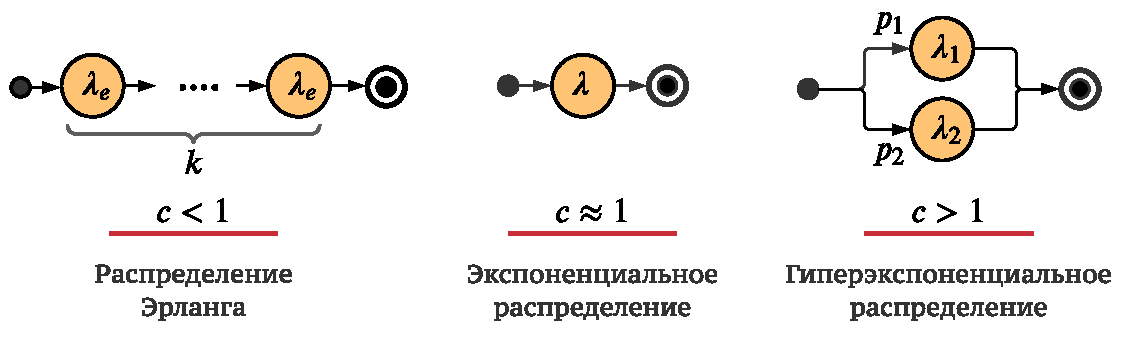
\includegraphics[width=0.9\textwidth]{chapter4/ch4_ph2.pdf}
  }
  \caption{PH-распределения, используемые при аппроксимации потоков по двум моментам}
  \label{fig:ch4_ph2}
\end{figure}

Если $c \approx 1$, то $\tilde{X} \sim Exp(\lambda)$. Матрицы MAP-потока $MAP(\tilde{D}_0, \tilde{D}_1)$ определяются с помощью выражения~\eqref{eq:ch4_map_ph_representation}.

Если $c > 1$, то $\tilde{X}$ -- гиперэкспоненциальное распределение с вероятностями $\overline{p} = (p_1, p_2)$ и интенсивностями $\overline{\lambda} = (\lambda_1, \lambda_2)$. Отметим, что интенсивности $\lambda_1, \lambda_2$ и вероятности $p_1$ и $p_2 = 1 - p_1$ определяются неоднозначно, так как ограничение на среднее и коэффициент вариации дают только два уравнения при трех неизвестных. Будем использовать следующее решение:
$$
\lambda_2 = \frac{1}{m_1} + 1,\quad \lambda_1 = \frac{m_1}{b \lambda_2 - m_1}, \quad p_1 = \frac{m_1^2}{b \lambda_2^2 - 2 m_1 \lambda_2 + 1},
$$
где $b = m_1^2(c^2 + 1) / 2$. Матрицы MAP-потока будут иметь вид:
$$
\tilde{D}_0 = \left(
    \begin{matrix}
        -\lambda_1 & 0\\
        0 & -\lambda_2
    \end{matrix}
    \right),\qquad
\tilde{D}_1 = \left(
    \begin{matrix}
        p_1 \lambda_1 & p_2 \lambda_1\\
        p_1 \lambda_2 & p_2 \lambda_2
    \end{matrix}
    \right).\qquad
$$

Наконец, если $c < 1$, то $\tilde{X}$ -- распределение Эрланга с числом состояний $k = \left[ 1 / c^2 \right]$ и параметром (интенсивностью каждого состояния) $\lambda_e = k / m_1$. Матрицы MAP-потока:
$$
\tilde{D}_0 = \left(
    \begin{matrix}
        -\lambda_e & \lambda_e & 0 & \cdots & 0\\
        0 & -\lambda_e & \lambda_e & \cdots & 0\\
        \vdots & \vdots & \vdots & \ddots & \vdots\\
        0 & 0 & 0 & \cdots &-\lambda_e
    \end{matrix}
    \right),\qquad
\tilde{D}_1 = \left(
    \begin{matrix}
        0 & 0 & \cdots & 0\\
        \vdots & \vdots & \ddots & \vdots\\
        0 & 0 & \cdots & 0\\
        \lambda_e & 0 & \cdots & 0
    \end{matrix}
    \right).\qquad
$$
Отметим, что коэффициент вариации $\tilde{c}$ может не совпадать в точности с исходным $c$ из-за округления.





%%% ~~~~~~~~~~~~~~~~
\subsection{Аппроксимация по трем моментам}\label{sec:ch4_approx_m3}
%%% ~~~~~~~~~~~~~~~~

Для большей точности результатов можно учитывать не только среднее значение $m_1$ и коэффициент вариации $c$ MAP-потока $X$, но и его коэффициент асимметрии $\gamma$. Существует ряд исследований, посвященных построению PH-распределений по трем и более моментам \cite{Osogami2006,Bobbio2005,Johnson1989,Telek2003,Horvath2013a,VandenBosch2000,Horvath2007,Schmickler1992}. Для упрощения задачи, поиск проводится не на всем классе PH-распределений, а на некотром его подмножестве. Например, в работах \cite{Bobbio2005,Telek2003} используются ациклические PH-распределения (APH), а в работе \cite{Johnson1989} используется распределение, представленное смесью двух распределений Эрланга с одинаковым числом фаз ($\text{ME}_\text{n}(2)$).

В общем случае PH-распределение можно найти для любого набора значений $m_1 > 0$, $c > 0$ и $\gamma > c - 1/c$, которыми может обладать какое-либо непрерывное положительное распределение \cite{Johnson1989}. Однако, порядок такого PH-распределения может быть очень большим. Например, в работе \cite{Aldous1987} было доказано, что при $c < 1$ самым малым порядком среди всех распределений с таким коэффициентом вариации  обладает распределение Эрланга. При этом порядок распределений Эрланга равен $1 / c^2$, то есть растет квадратично при приближении коэффициента вариации к нулю. Таким образом, если хочется получить PH-распределение с ограниченным числом фаз, то неизбежно приходится также ограничивать и область значений параметров $m_1, c, \gamma$ (особенно в области $c < 1$). Если же нужно иметь возможность получить PH-распределение для произвольных $m_1, c, \gamma$, то приходится смириться с неограниченным ростом сложности такого распределения.

\begin{figure}[h]
  \centerfloat{
    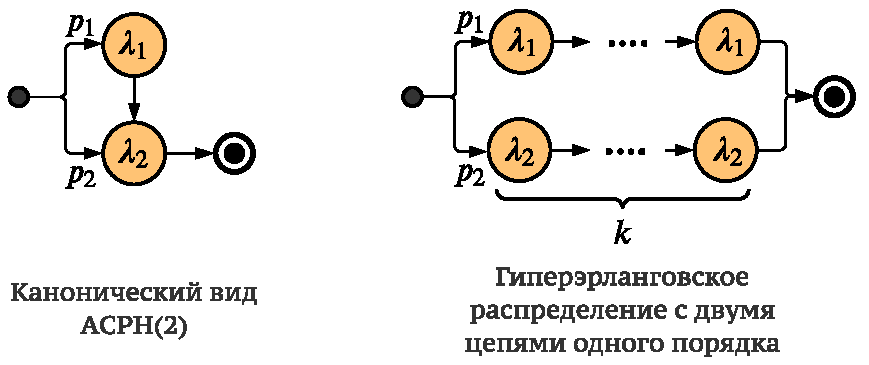
\includegraphics[width=0.7\textwidth]{chapter4/ch4_ph3.pdf}
  }
  \caption{Ациклическое PH-распределение с двумя состояниями ACPH(2) и гипер-Эрланговское распределение с двумя распределениями Эрланга одинакового порядка, используемые при аппроксимации потоков по трем моментам.}
  \label{fig:ch4_ph3}
\end{figure}

В диссертационной работе будут использоваться два простых метода. Во-первых, попытаемся построить ациклическое PH-распределение второго порядка (ACPH(2)) в каноническом виде (см. рис.~\ref{fig:ch4_ph3}, левая схема) с помощью метода, описанного в работе Telek и Heindl \cite{Telek2003}. Если моменты не попадают в область существования ACPH(2) (см. рис.~\ref{fig:ch4_ph_feasible_regions}), то используем более универсальный метод, предолженный Johnson и Taafe \cite{Johnson1989}, с помощью которого PH-распределение ищется в виде смеси двух распределений Эрланга $ME_n(2)$ (см. рис.~\ref{fig:ch4_ph3}, правая схема). Опишем эти методы подробнее.

\begin{figure}[h]
  \centerfloat{
    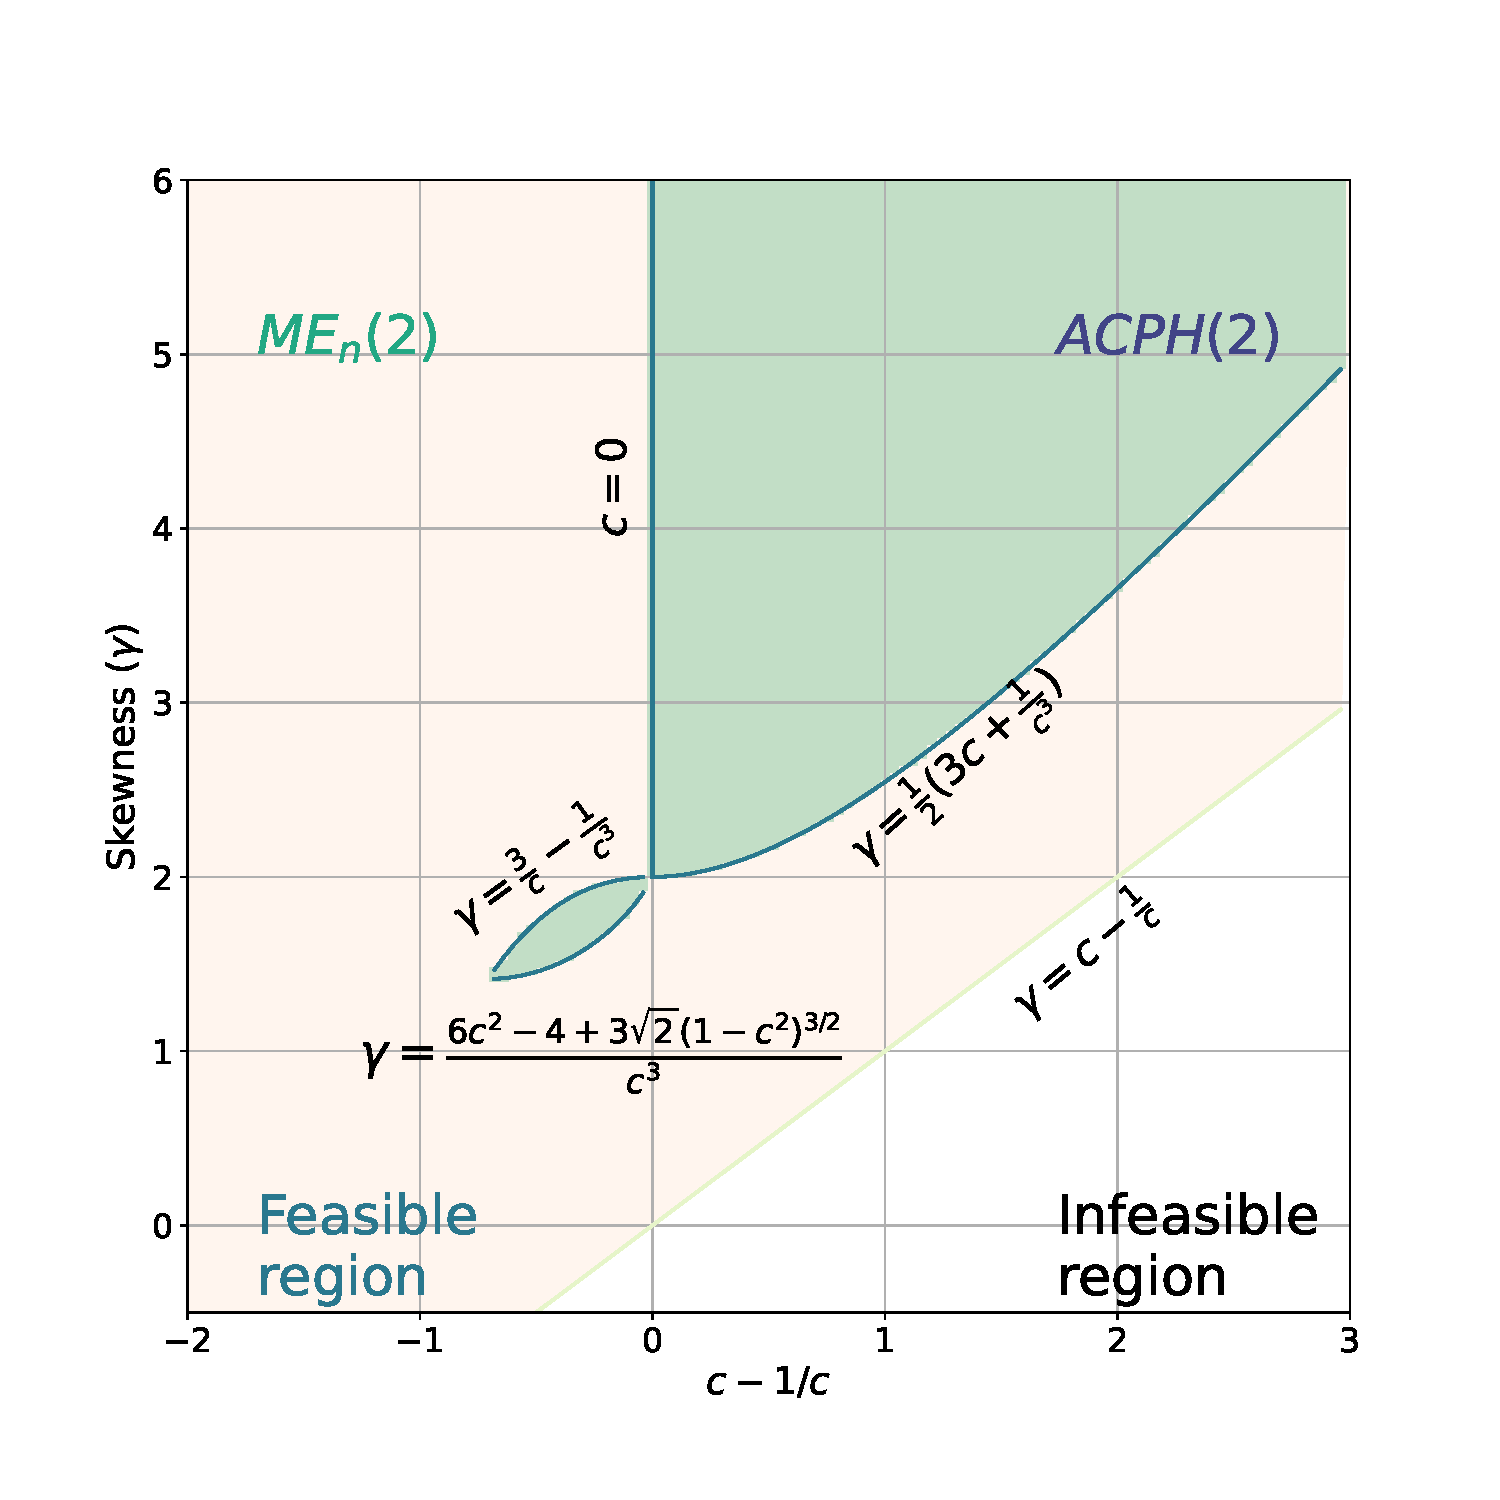
\includegraphics[width=0.8\textwidth]{chapter4/ch4_ph_feasible_regions.pdf}
  }
  \caption{Области существования PH-распределений. Зеленым цветом показана область существования ACPH(2) \cite{Telek2003}, розовым -- произвольных PH-распределений, в частности $\text{ME}_\text{n}(2)$ \cite{Johnson1989}. Ниже линии $\gamma = c - 1/c$ PH-распределений не существует.}
  \label{fig:ch4_ph_feasible_regions}
\end{figure}

Ациклические PH-распределения второго порядка ACPH(2) существуют в ограниченной области \cite{Telek2003}. Границы области можно выразить через коэффициенты асимметрии $\gamma$ и вариации $c$:

\begin{equation}
    \label{eq:ch4_acph2_existance}
    \begin{matrix}
        \frac{6c^2 - 4 + 3\sqrt{2}(1 - c^2)^{\frac{3}{2}}}{c^3} \leqslant \gamma \leqslant \frac{3c^2 - 1}{c^3}, & \frac{1}{\sqrt{2}} \leqslant c \leqslant 1\\
        \frac{1}{2}(3c + \frac{1}{c^3}) \leqslant \gamma, & c > 1
    \end{matrix}
\end{equation}
При $c < 1/\sqrt{2}$ распределений ACPH(2) не существует. Область существования показана на рис.~\ref{fig:ch4_ph_feasible_regions}.

Распределение ACPH(2) определяется тремя параметрами $\lambda_1$, $\lambda_2$ и $p_1$ (вероятность $p_2 = 1 - p_1$), см. рис.~\ref{fig:ch4_ph3}. Их можно вычислить следующим  образом:

\begin{equation}
    \label{eq:ch4_acph2_params}
    p = \frac{-B + 6 m_1 D + \sqrt{A}}{B + \sqrt{A}}, \quad
    \lambda_{1} = \frac{B - \sqrt{A}}{C}, \quad
    \lambda_{2} = \frac{B + \sqrt{A}}{C}
\end{equation}
где $D = 2m_1^2 - m_2$, $C = 3 m_2^2 - 2 m_1 m_3$, $B = 3 m_1 m_2 - m_3$ и $A = B^2 - 6 C D$. Здесь $m_i = \mathbb{E}X^i$ -- $i$-й момент случайной величины. Моменты $m_2$ и $m_3$ можно выразить через коэффициент вариации $c$ и асимметрии $\gamma$ как $m_2 = m_1 c^2 + m_1^2$ и $m_3 = m_1^3 (c^3 \gamma + 3 c^2 + 1)$. Матрица $S$ и вектор начального распределения $\overline{\tau}$ для ACPH(2) будут иметь следующий вид:

\begin{equation}
    \label{eq:ch4_acph2_ph_tau}
    S = \left(\begin{matrix}
        -\lambda_1 & \lambda_1 \\
        0 & -\lambda_2
    \end{matrix}\right),
    \qquad
    \overline{\tau} = \left(\begin{matrix}
        p_1 & 1 - p_1
    \end{matrix}\right).
\end{equation}

Если коэффициенты $c$ и $\gamma$ аппроксимируемого потока не удовлетворяют ограничениями \eqref{eq:ch4_acph2_existance}, то будем искать PH-распределение в классе $\text{ME}_\text{n}(2)$. В отличие от узкого класса ACPH(2), распределения $\text{ME}_\text{n}(2)$ существуют для любого значения $\gamma > c - 1/c$, то есть их область существования совпадает с областью существования произвольных PH-распределений \cite{Johnson1989}. Соотношение между областями существования ACPH(2) и $\text{ME}_\text{n}(2)$ показано на рис.~\ref{fig:ch4_ph_feasible_regions}. Распределения $\text{ME}_\text{n}(2)$ представляют собой смесь двух распределений Эрланга одинакового порядка $n$ с вероятностями $p_1$ и $p_2 = 1 - p_1$. Распределения Эрланга имеют параметры $\lambda_1$ и $\lambda_2$ (см. рис.~\ref{fig:ch4_ph3}). Минимальный порядок $n^*$ распределений Эрланга в $\text{ME}_\text{n}(2)$ для заданных значений $c$ и $\gamma$ определяется согласно утверждению 4 из работы \cite{Johnson1989}:

\begin{equation}
    \label{eq:ch4_men2_min_n}
    n^* = \lceil \max \lbrace
            \frac{1}{c^2}, \;
            \frac{-\gamma + 1/c^3 + 1/c + 2c}{\gamma - (c - 1/c)}
        \rbrace \rceil
\end{equation}

После выбора $n \geqslant n^*$ можно вычислить параметры $\lambda_1$, $\lambda_2$ и $p_1$. Способ вычисления описан в теореме 3 \cite{Johnson1989}:

\begin{equation}
    \label{eq:ch4_men2_params}
    \lambda_i^{-1} = \frac{-B \pm \sqrt{B^2 - 4 A C}}{2 A}, \qquad
    p_1 = \frac{m_1/n - \lambda_2^{-1}}{\lambda_1^{-1} - \lambda_2^{-1}},
\end{equation}
где
\begin{equation}
    \label{eq:ch4_men2_params_aux}
    \begin{aligned}
        A &= n(n+2) m_1 y\\
        B &= -\left( nx + \frac{n(n+2)}{n+1}y^2 + (n+2) m_1^2 y \right)\\
        C &= m_1 x\\
        x &= m_1 m_3 - \frac{n+2}{n+1} m_2^2\\
        y &= m_2 - \frac{n+1}{n} m_1^2
    \end{aligned}
\end{equation}
Матрица $S$ и вектор начального распределения $\overline{\tau}$ для PH-распределения из класса $\text{ME}_\text{n}(2)$ будут иметь вид:

\begin{equation}
    \label{eq:ch4_men2_ph_tau}
    \begin{aligned}
        S &= \left(\begin{blockarray}{cccc|cccc}
            -\lambda_1 & \lambda_1 & & & & & & \\
             & -\lambda_1 & \lambda_1 & & & & & \\
             & & \ddots & & & \text{\Huge0} & & \\
            & & & -\lambda_1 & & & & \\
            \cline{1-8}
             & & & & -\lambda_2 & \lambda_2 & & \\
             & & & & & -\lambda_2 & \lambda_2 & \\
            & \text{\Huge0} & & & & & \ddots &\\
            & & & & & & & -\lambda_2
        \end{blockarray}\right)\\
        \overline{\tau} &= (\begin{matrix}
        p_1 & 0 & \dots & 0 & | & 1 - p_1 & 0 & \dots & 0
        \end{matrix}).
    \end{aligned}
\end{equation}

В работе Johnson и Taafe~\cite{Johnson1989} приведен подробный анализ класса $\text{ME}_\text{n}(2)$, а также есть рекомендации, что делать, если $\lambda_1 / \lambda_2 \gg 1$, $\lambda_1 / \lambda_2 \ll 1$ или $p_i \approx 1$. Например, небольшое увеличение $n$ может сблизить $\lambda_1$ и $\lambda_2$. Хотя некоторые из рекомендаций были реализованы, в диссертационной работе будем использовать простейшую форму построения $\text{ME}_\text{n}(2)$, так как хотелось бы избежать как дополнительного роста размерности, так и существенных отклонений в коэффициентах вариации и асимметрии.

Объединяя все изложенное выше, будем искать PH-распределение по трем моментам следующим образом.

\begin{enumerate}
    \item Если $c \approx 1$, $\gamma \approx 2$, то строим экспоненциальное распределение с $\lambda = 1/m_1$. Матрицы искомого MAP-потока будут иметь вид~\eqref{eq:ch4_map_from_exp}.
    \item Если коэффициенты $c$ и $\gamma$ удовлетворяют условиям $c > 1/\sqrt{2}$ и~\eqref{eq:ch4_acph2_existance}, то строим распределение ACPH(2):
    \begin{enumerate}
        \item Рассчитываем параметры $\lambda_1$, $\lambda_2$ и $p_1$ с помощью~\eqref{eq:ch4_acph2_params}.
        \item Строим матрицу $S$ и вектор $\overline{\tau}$ с помощью~\eqref{eq:ch4_acph2_ph_tau}.
    \end{enumerate}
    \item Если для заданных $c$ и $\gamma$ распределения ACPH(2) не существует, то строим распределение $\text{ME}_\text{n}(2)$:
    \begin{enumerate}
        \item Рассчитываем параметры $\lambda_1$, $\lambda_2$ и $p_1$ с помощью~\eqref{eq:ch4_men2_params} и~\eqref{eq:ch4_men2_params_aux}.
        \item Строим матрицу $S$ и вектор $\overline{\tau}$ с помощью~\eqref{eq:ch4_men2_ph_tau}.
    \end{enumerate}
    \item Для найденного распределения $PH(S, \overline{\tau})$ строим матрицы MAP-потока $D_0$ и $D_1$ с помощью выражения \eqref{eq:ch4_map_ph_representation}.
\end{enumerate}

В завершение отметим, что вместо алгоритмов из работ~\cite{Telek2003} и~\cite{Johnson1989} можно использовать любые другие алгоритмы, позволяющие построить PH-распределение по трем моментам.



%%% ~~~~~~~~~~~~~~~~
\subsubsection{Аппроксимация по трем моментам и автокорреляции}\label{sec:ch4_approx_m3_lag1}
%%% ~~~~~~~~~~~~~~~~

Последний вариант аппроксимаций, который будет рассматриваться в диссертационном исследовании, это аппроксимация MAP-потока другим MAP-потоком с теми же первыми тремя моментами и коэффициентом автокорреляции с лагом 1, то есть корреляцией между соседними интервалами между возникновением событий в MAP-потоке. Как и ранее, ключевая идея здесь заключается в том, чтобы понизить размерность MAP-потока: если учитывать только ограниченный набор характеристик, то есть шанс получить MAP-поток меньшего размера.

Для поиска аппроксимирующего MAP-потока будем пользоваться методом, предложенным Horvath и соавторами в работе~\cite{Horvath2005}. Согласно этому подходу, матрицы $D_0$ и $D_1$ ищутся независимо по значениям моментов и коэффициентам автокорреляции. Метод основан на том, что стационарное распределение MAP-потока, определяющее его моменты, есть $PH(D_0,\, \overline{\alpha})$, где $\overline{\alpha}$ "--- стационарное распределение вложенной по моментам появления событий цепи с матрицей $P = (-D_0)^{-1} D_1$. Поэтому можно найти матрицу $D_0$ и вектор $\overline{\alpha}$, используя любой из ранее описанных методов для поиска PH-распределений, а информацию о значениях коэффициентов автокорреляции использовать для поиска матрицы $D_1$.

В общем случае поиск элементов матрицы $D_1 \in \mathbb{R}^{W \times W}$ по известным коэффициентам автокорреляции с лагами $i=1, 2, \dots, L$ можно сформулировать как задачу оптимизации:

\begin{equation}
    \label{eq:ch4_map_lag_opt_criterion}
    D_1 = \argmin \limits \sum\limits_{i=1}^L w_i \left(\frac{\lambda \overline{\pi} (-D_0)^{-k} D_1^k (-D_0)^{-1} \overline{\mathbf{1}} - 1}{2 \overline{\pi} (-D_0)^{-1} \overline{\mathbf{1}} - 1} - \rho_i \right)^2
\end{equation}
с ограничениями
\begin{equation}
    \label{eq:ch4_map_lag_opt_constraints}
    \begin{aligned}
        &D_1 \overline{1} = -D_0 \overline{1}\\
        &\overline{\alpha} (-D_0)^{-1} D_1 = \overline{\alpha}\\
        &\{D_1\}_{ij} \geqslant 0,\quad i, j = \overline{1, W}.
    \end{aligned}
\end{equation}
Здесь $w_i$, $i = 1, 2, \dots, L$ "--- веса, с помощью которых можно регулировать важность приближения того или иного момента. Отметим, что ограничения \eqref{eq:ch4_map_lag_opt_constraints} линейны относительно элементов матрицы $D_1$.
Кроме ограничений \eqref{eq:ch4_map_lag_opt_constraints} также нужно убедиться, что управляющая цепь с генератором $D = D_0 + D_1$ неприводима.

Ограничением применения метода является то, что диапазон возможных значений $\rho_i$ определяется выбором стационарного PH-распределения. В общем случае, для заданных $m_1$, $c$ и $\gamma$ PH-распределение определяется неоднозначно, его вид зависит от используемых методов. Возможна ситуация, когда PH-распределение найти удалось, а матрицу $D_1$ для MAP-потока с заданными коэффициентами корреляции $\rho_i$ "--- нет, хотя MAP-поток с искомыми параметрами существует.

Пусть $L = 1$. Функция
$$
\rho(D_1) = \frac{\lambda \overline{\pi} (-D_0)^{-1} D_1 (-D_0)^{-1} \overline{\mathbf{1}} - 1}{2 \overline{\pi} (-D_0)^{-1} \overline{\mathbf{1}} - 1},
$$
принимающая значение коэффициента корреляции с лагом 1, представляет собой линейную комбинацию элементов матрицы $D_1$. Значит, для нахождения минимального $\underline{\rho_1}$ и максимально $\hat{\rho}_1$ значения $\rho_1$ при заданной матрице $D_0$ можно использовать симплекс-метод:

\begin{equation}
    \label{eq:ch4_approx_map_rho_boundaries}
    \begin{aligned}
        \hat{\rho}_1 &= \max \rho(D_1)\\
        \underline{\rho_1} &= \min \rho(D_1)
    \end{aligned}
\end{equation}
при ограничениях \eqref{eq:ch4_map_lag_opt_constraints}. Пользуясь выпуклостью задачи линейного программирования, если заданное значение $\rho_1 \in [\underline{\rho_1}, \hat{\rho}_1]$, то матрицу $D_1$ можно найти, решая систему линейных алгебраических уравнений относительно элементов матрицы $D_1$:

\begin{equation}
    \label{eq:ch4_map_lag_opt_ales}
    \begin{cases}
        D_1 \overline{1} &= -D_0 \overline{1}\\
        \overline{\alpha} (-D_0)^{-1} D_1 &= \overline{\alpha}\\
        \frac{\lambda \overline{\pi} (-D_0)^{-1} D_1 (-D_0)^{-1} \overline{\mathbf{1}} - 1}{2 \overline{\pi} (-D_0)^{-1} \overline{\mathbf{1}} - 1} &= \rho_1
    \end{cases}
\end{equation}
Отметим, что если порядок искомого MAP-потока $W > 1$, то у системы будет бесконечное множество решений. Если $\rho_1 > \hat{\rho}$ или $\rho_1 < \underline{\rho_1}$, то будем брать ту матрицу $D_1$, которая соответствует найденному ранее экстремуму.

На практике иногда возникает ситуация, когда результатом решения проблемы \eqref{eq:ch4_map_lag_opt_criterion} является такая матрица $D_1$, что цепь Маркова с генератором $D = D_0 + D_1$ не является неприводимой. Для быстрой проверки неприводимости удобно использовать алгоритм Тарьяна \cite{tarjan72} для поиска сильно-связных компонент графа. Сильно-связная компонента "--- это такой набор вершин графа, в котором из каждой вершины можно попасть в любую другую вершину. Если цепь состоит из единственной сильно-связной компоненты, то она является неприводимой. Для повышения качества результатов, при построении графа будем игнорировать переходы между состояниями цепи, вероятности которых крайне малы. Чтобы подчеркнуть важность проверки на неприводимость отметим, что в ходе численных экспериментов, которые будут обсуждаться далее, около 16\% всех построенных MAP-потоков имели не неприводимые цепи.

Если полученная цепь $D = D_0 + D_1$ не является неприводимой, то есть несколько возможных действий. Во-первых, так как проблемы \eqref{eq:ch4_map_lag_opt_criterion} и \eqref{eq:ch4_map_lag_opt_ales} могут иметь множество решений, можно попытаться найти другую матрицу $D_1$ с той же матрицей $D_0$ и вектором $\overline{\alpha}$. Во-вторых, можно попытаться найти другое распределение $PH(D_0, \overline{\alpha})$ с теми же моментами. Для этого можно использовать другой метод, или ослабить требования точности на третий и/или второй моменты. В-третьих, можно найти другую матрицу $D_1$, для которой $\rho(D_1)$ будет близко, но не равно в точности значению $\rho_1$. В нашей работе мы используем третий подход.

В завершение отметим, что существуют и другие подходы к построению MAP-потоков по моментам и коэффициентам автокорреляции, например~\cite{TelekHorvath2007,Bodrog2010}. Кроме того, MAP-потоки можно строить по выборке (ее можно получить из аппроксимируемого потока), используя EM-процедуру \cite{Horvath2013,Ephraim2009,Buchholz2003}.


%%% ~~~~~~~~~~~~~~~~
\subsection{Сложность и применимость метода}\label{sec:ch4_approx_complexity}
%%% ~~~~~~~~~~~~~~~~

Хотя метод понижения размерности позволяет находить оценки характеристик сетей массового обслуживания с произвольно большим числом узлов, он, как и метод Монте-Карло, не может обеспечить очень быстрый расчет. Проблема состоит в том, что размерности потоков нельзя сделать сколь угодно низкими. Хорошо известно \cite{Aldous1987}, что если коэффициент вариации $c$ искомого распределения меньше единицы, то самое малое число состояний $K = \lceil 1 / c^2 \rceil $ будет у распределения Эрланга. Таким образом, неограниченного роста размерности невозможно избежать даже тогда, когда для приближения используется всего два первых момента. Пусть $\hat{c} = \min\{c_1, c_2, \dots, c_{N-1}\}$ "--- минимальный коэффициент вариации среди всех выходных потоков кроме последнего узла, который здесь не играет роли, и $\hat{W} = \max\{\lceil 1 / \hat{c}^2 \rceil, W\}$. Тогда сложность алгоритма можно оценить как $\mathcal{O}(N (\hat{W}MV)^3 )$. Конечно, это гораздо лучше экспоненциального роста сложности точного алгоритма, но все равно очень много. Еще стоит отметить, что хотя порядок PH-распределений слабее зависит от коэффициента асимметрии, чем от коэффициента вариации (см., например, \cite{Johnson1989}), для точного совпадения третьего момента и коэффициента корреляции также может потребоваться увеличить размерность. Наконец, поиск матрицы $D_1$ даже по коэффициенту корреляции с лагом один требует в общем случае решать задачу оптимизации, и это приходится делать для каждого выходного потока.




%%%%%%%%%%%%%%%%%%%%%%%%%%%%%%%%%%%%%%%%%%%%%%%%%%%%%%%%%%%%%%%%%%%%%%%%%%%%%%%%
\section{Моделирование задержки в канале}\label{sec:ch4_channel}
%%%%%%%%%%%%%%%%%%%%%%%%%%%%%%%%%%%%%%%%%%%%%%%%%%%%%%%%%%%%%%%%%%%%%%%%%%%%%%%%

В диссертационной работе предметом исследования является многошаговая беспроводная сеть сбора данных с камер или RFID-считывателей, работающая под управлением протокола IEEE 802.11 и передающая трафик в одном направлении. Будем считать, что все станции этой сети работают в одном канале, антенны у всех станций имеют круговую диаграмму, и станции расположены таким образом, что передачу любой станции могут получить только ее непосредственные соседи (см. рис.~\ref{fig:ch4_network_collisions}). В такой сети коллизия на станции $S_i$ возникнет при одновременной передаче ее соседей, то есть когда станция $S_{i-1}$ будет вести передачу станции $S_i$, а станция $S_{i+1}$ "--- станции $S_{i+2}$: из-за круговой диаграммы и использования общего канала, последнюю передачу также получит станция $S_i$.

\begin{figure}[h]
  \centerfloat{
    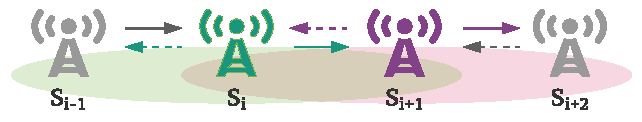
\includegraphics[width=0.5\textwidth]{chapter4/ch4_network_collisions}
  }
  \caption{Области видимости станций многошаговой беспроводной сети}
  \label{fig:ch4_network_collisions}
\end{figure}

Для моделирования длительности передачи пакетов в беспроводном канале с помощью PH-распределений нужно знать моменты этого распределения или иметь выборку длительностей. В диссертационном исследовании будем пользоваться методом восстановления PH-распределения по трем моментам, описанном в разделе~\ref{sec:ch4_approx_m3}, основанном на работах Johnson и Taafe~\cite{Johnson1989} и Telek и Heindl~\cite{Telek2003}.

Для получения оценок моментов распределения длительностей передачи пакетов можно использовать аналитические или имитационные модели каналов. Например, в работах \cite{QS_ICAAPSP2020,QS_ITMM2019} время передачи моделировалось с помощью полумарковского процесса для насыщенного режима, а также использовались простые имитационные модели каналов CSMA/CA для ненасыщенного режима. Если в качестве модели канала используется полумарковский процесс, то через вычисление функции генерации моментов можно получить значения математического ожидания и дисперсии для построенного этого процесса (см., например, работу Sakurai~\cite{Sakurai2007}). В результатах, представленных в диссертационном исследовании, использовалась более точная имитационная модель канала IEEE 802.11 из системы моделирования NS-3.

Длительность передачи в беспроводном канале определяется не только настройками приемников и передатчиков, но и вероятностью коллизий, которая зависит от числа конкурирующих станций. В исследуемой многошаговой сети станции работают в одном канале, поэтому вероятность коллизий зависит от положения станции внутри сети. Таким образом, для получения достаточно точных оценок нужно использовать разные PH-распределения на разных приборах.

\begin{figure}[h]
  \centerfloat{
    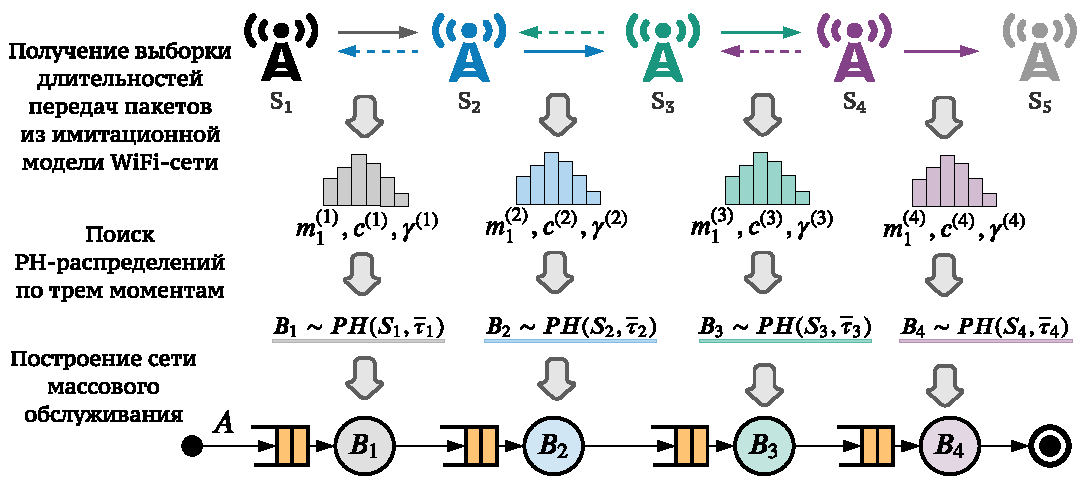
\includegraphics[width=0.9\textwidth]{chapter4/ch4_channel_model_schema}
  }
  \caption{Схема моделирования каналов беспроводной сети}
  \label{fig:ch4_channel_model_schema}
\end{figure}

Рассмотрим сеть, состоящую из пяти станций (см. рис.~\ref{fig:ch4_channel_model_schema}). Возможны четыре различных случая:

\begin{enumerate}
  \item Канал $S_1 \rightarrow S_2$: канал занят, если станция $S_2$ ведет передачу; возможна коллизия с передачами станции $S_3$.
  \item Канал $S_2 \rightarrow S_3$: канал занят, если станции $S_1$ или $S_3$ ведут передачу; возможна коллизия с передачами станции $S_4$.
  \item Канал $S_3 \rightarrow S_4$: канал занят, если станция $S_2$ или $S_4$ ведут передачу; станция $S_5$ "--- конечная, далее не передает, поэтому коллизий нет.
  \item Канал $S_4 \rightarrow S_5$: канал занят, если станция $S_3$ ведет передачу; коллизий нет.
\end{enumerate}

Для каждого из этих каналов строится отдельное PH-распределение $B_1$, $B_2$, $B_3$ и $B_4$ (номер распределения совпадает с номером станции-отправителя). Если сеть содержит меньше станций, то и распределений потребуется меньше.

\begin{figure}[h]
  \centerfloat{
    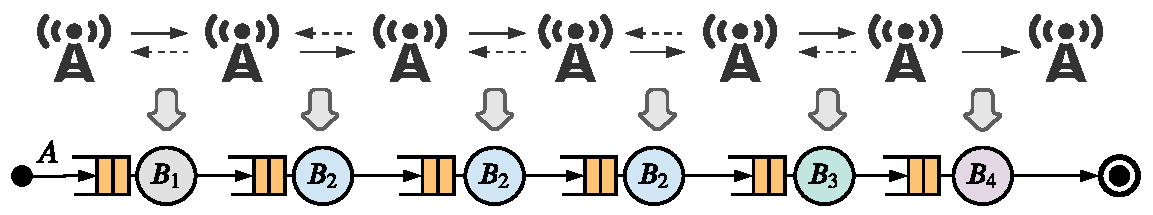
\includegraphics[width=0.9\textwidth]{chapter4/ch4_network_model_schema}
  }
  \caption{Схема моделирования беспроводной сети с произвольным числом станций}
  \label{fig:ch4_network_model_schema}
\end{figure}

Если добавятся промежуточные станции, то новые каналы будут испытывать нагрузку, аналогичную каналу $S_2 \rightarrow S_3$, поэтому сеть можно моделировать с помощью тех же распределений $B_1$, $B_2$, $B_3$ и $B_4$ (см. рис.~\ref{fig:ch4_network_model_schema}).



%%%%%%%%%%%%%%%%%%%%%%%%%%%%%%%%%%%%%%%%%%%%%%%%%%%%%%%%%%%%%%%%%%%%%%%%%%%%%%%%
\section{Численное исследование эффективности метода аппроксимации потоков}
%%%%%%%%%%%%%%%%%%%%%%%%%%%%%%%%%%%%%%%%%%%%%%%%%%%%%%%%%%%%%%%%%%%%%%%%%%%%%%%%

Для исследования эффективности метода вычисления оценок характеристик тандемной сети массового обслуживания, был проведен ряд численных экспериментов на случайном наборе данных. Входящий набор данных включал 2500 сетей со случайными значениями среднего времени обслуживания, коэффициентов вариации и асимметрии интервалов между пакетами и времен обслуживания, коэффициента автокорреляции входящего MAP-потока с единичным лагом, случайными емкостями очередей и случайным числом станций в сети. На всех наборах были найдены решения методом Монте-Карло и всеми методами аппроксимации потоков, описанных в разделе~\ref{sec:ch4_approx}. На тех входных данных, на которых это было возможно, было найдено точное решение.

Сначала рассмотрим, как был сгенерирован набор входных данных для исследования методов аппроксимации выходящих потоков. Затем приведем результаты измерения ошибок, возникающих при использовании этих методов. В завершение покажем, как меняется точность метода Монте-Карло при увеличении числа сгенерированных пакетов.


\subsection{Построение набора данных для исследования}

Для проведения численных экспериментов были сгенерированы 2000 входных параметров со случайными средними временами обслуживания, коэффициентами вариации интервалов между пакетами $c_a$ и обслуживания $c_s$, коэффициентами асимметрии поступления $\gamma_a$ и обслуживания $\gamma_s$, коэффициентами автокорреляции входящего потока $\rho_l$, числом узлов в сети и емкостью очередей. Интенсивность (и, соответственно, средний интервал) входящего потока во всех случаях полагалась равной единице, поэтому коэффициент загрузки первого узла был равен $m_s / m_a = m_s$. Границы значений параметров для стандартного генератора показаны в табл.~\ref{tab:ch4_results_approx_input_range}. Отметим, что так как емкости очередей в системе ограничены, и переполняющие очередь пакеты теряются, исследовать системы с коэффициентом загрузки $m_s / m_a > 1$ корректно. Для построения PH-распределений времени обслуживания по выбранным случайным параметрам $m_s, c_s, \gamma_s$ использовались методы, описанные в разделах \ref{sec:ch4_approx_m1}, \ref{sec:ch4_approx_m2} и \ref{sec:ch4_approx_m3}, а для построения MAP-потоков по $m_a \equiv 1, c_a, \gamma_a, \rho_1$ "--- метод из раздела \ref{sec:ch4_approx_m3_lag1}.

\begin{table}[h]
    \caption{\label{tab:ch4_results_approx_input_range} Граничные значения параметров для исследования методов аппроксимации потоков.}
    \begin{tabular}{|c|cc|cc|}
        \hline
        \multirow{2}{*}{Параметр}
          &\multicolumn{2}{c|}{Стандартный генератор}&\multicolumn{2}{c|}{Простые распределения}\\
                        &Мин.   &Макс.    &Мин.   &Макс.\\
        \hline
        $m_s$           &0,1       &1,5        &0,1        &1,5\\
        $c_s$,$c_a$     &0,5       &4,0        &0,5        &4,0\\
        $\gamma_{a,s}$  &$c_{a,s} - 1/c_{a,s}$ &6.0    &\multicolumn{2}{c|}{Не используется}\\
        $\rho_1$        &\multicolumn{4}{c|}{Границы рассчитываются как решение задачи \eqref{eq:ch4_approx_map_rho_boundaries}}\\
        Размер сети $N$ &1          &10        &3           &10\\
        Емкость очереди $M$ &0      &10        &0           &3\\
        \hline
    \end{tabular}
\end{table}


Сложность итерационного алгоритма для точного расчета характеристик сети растет экспоненциально с ростом числа узлов. Для получения точного решения требовалось, чтобы порядок матриц выходящего потока с последнего узла был достаточно мал. В противном случае матрицы могут просто не поместиться в оперативной памяти или потребуют слишком много времени для выполнения операции обращения и получения решения системы линейных уравнений. Следуя этой логике, для получения точного решения использовались только те входные данные, на которых матрица потока обслуженных заявок на последнем узле имеет порядок не выше 8000. После такого отсева оставалось слишком мало входных наборов, поэтому дополнительно были сгенерированы 1000 наборов входных параметров, в которых использовались более простые распределения и меньшие очереди: PH-распределение времени обслуживаня и стационарное PH-распределение MAP-потоков строились по первым двум моментам (см. раздел \ref{sec:ch4_approx_m2}), а не трем, длина очереди выбиралась из меньшего диапазона, а число узлов ограничивалось снизу, см. табл.~\ref{tab:ch4_results_approx_input_range}.

\begin{figure}[h]
  \centerfloat{
    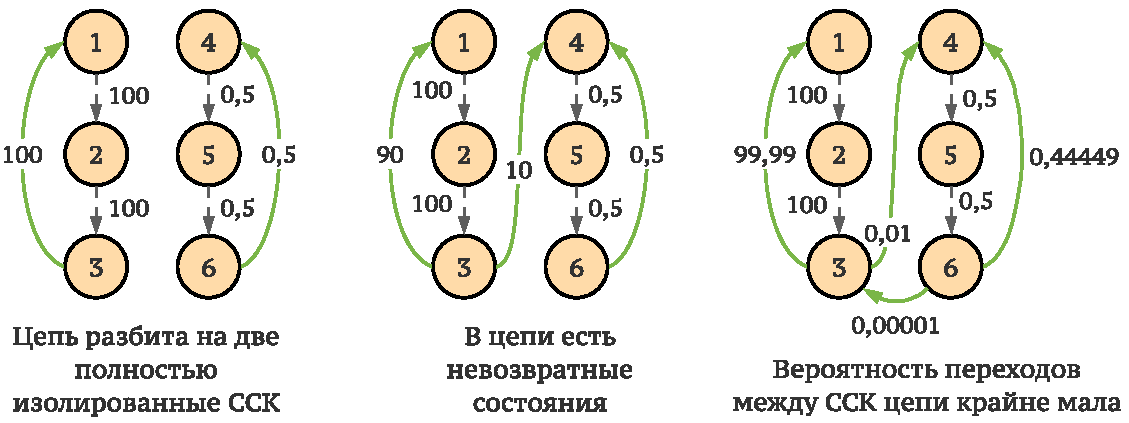
\includegraphics[width=0.8\textwidth]{chapter4/ch4_results_bad_maps.pdf}
  }
  \caption{Примеры отсеиваемых MAP-потоков. На стрелках показана интенсивность переходов. Сплошные линии "--- переходы матрицы $D_1$, пунктирные "--- $D_0$}.\label{fig:ch4_results_bad_maps}
\end{figure}

В итоге были получены 3000 входных наборов. Как было отмечено в разделе \ref{sec:ch4_approx_m3_lag1}, иногда построенные MAP-потоки не были неприводимыми. В некоторых случаях пространство состояний распадалось на две сильно связные компоненты, соответствующие цепочкам Эрланга. Примеры <<плохих>> MAP-потоков показаны на рис.~\ref{fig:ch4_results_bad_maps}. Если бы такие потоки использовались при расчете методом Монте-Карло, были бы получены некорректные результаты. Например, запуская имитационную модель (реализацию метода Монте-Карло) два раза, и выбирая в качестве начального состояния MAP-потока состояние сначала из первой, а затем из второй компоненты, по сути рассматривались бы два разных потока, так как попасть из состояний одной компоненты в другую невозможно, и, таким образом, были бы получены разные результаты. Для того, чтобы быстро отсеить <<плохие>> потоки, был использован алгоритм Тарьяна поиска сильно-связных компонентов в графе~\cite{tarjan72}. Множество вершин такого графа совпадает с множеством состояний цепи, а дуга между состояниями $i$ и $j$ в графе есть только в том случае, если вероятность перехода во вложенной цепи $\mathbb{P}\{X_{n+1} = j | X_n = i\} > 10^{-3}$. Нижняя граница нужна, чтобы отсеить случаи, когда переходы между компонентами есть, но крайне маловероятны: такие переходы срабатывают редко, а переход по ним может существенно изменить оценки характеристик, поэтому для получения устойчивых результатов нужно моделировать огромное число событий.

\begin{figure}[h]
  \centerfloat{
    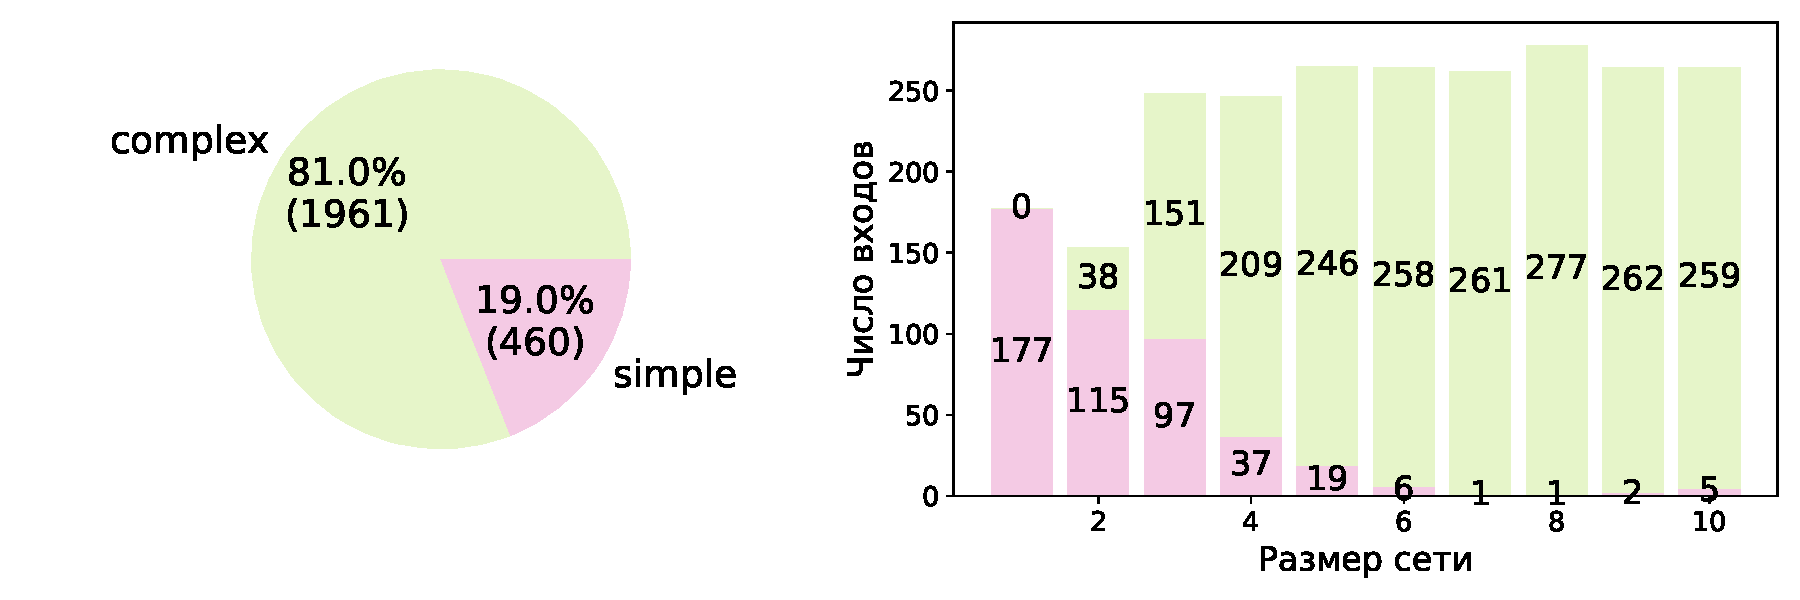
\includegraphics[width=0.9\textwidth]{chapter4/ch4_results_complexity_split}
  }
  \caption{Разбиение наборов входных данных на простые и сложные.}\label{fig:ch4_results_complexity_split}
\end{figure}

В результате отсеивания было удалено 579 входных наборов, то есть 19,3\% данных. Оставшиеся наборы были поделены на <<простые>> и <<сложные>>: к простым наборам были отнесены те, для которых порядок выходящего потока, равный $\hat{W}_N = W(V(M+2))^N$, не превосходил 8000, а все остальные "--- к сложным. Ожидаемо, большинство простых наборов соответствовали сетям малого размера, см. рис.~\ref{fig:ch4_results_complexity_split}. Так как для больших сетей простых наборов оказалось слишком мало, в дальнейшем точное решение искалось только для тех простых наборов, в которых длина сети не превышала 5.

\begin{figure}[h]
  \centerfloat{
    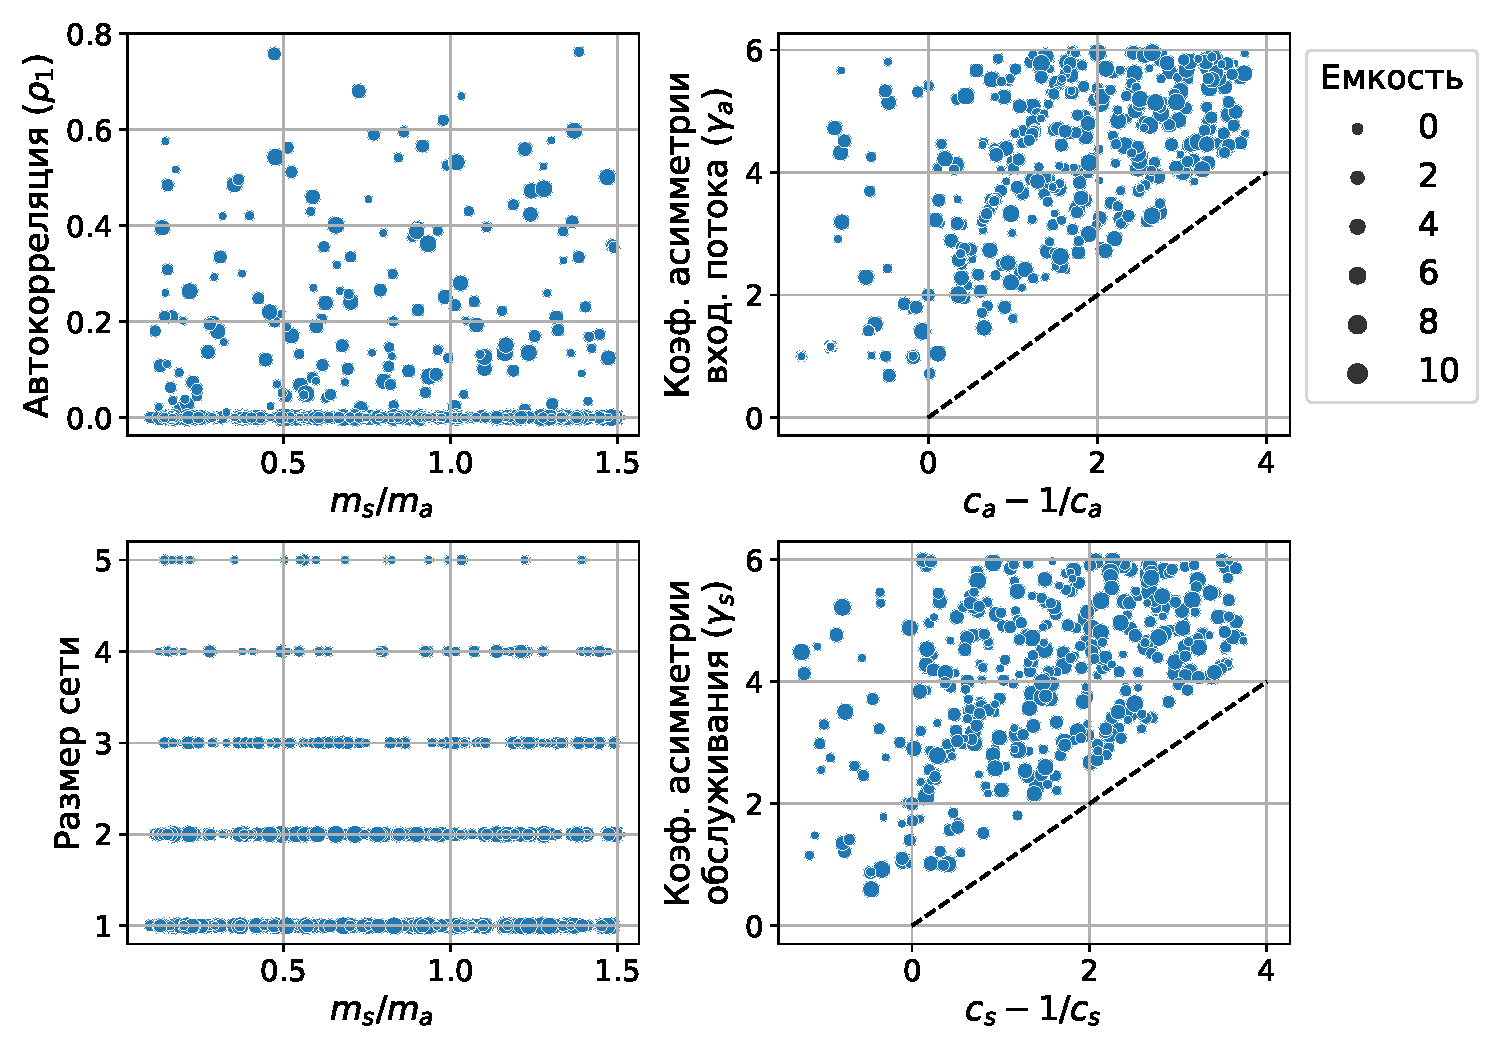
\includegraphics[width=0.8\textwidth]{chapter4/ch4_results_input_scatter}
  }
  \caption{Диаграммы разброса для различных сочетаний параметров в наборах простых входных данных. Размеры кругов соответствуют емкостям очередей.}\label{fig:ch4_results_input_scatter}
\end{figure}

На рис.~\ref{fig:ch4_results_input_scatter} показаны диаграммы разброса различных параметров в наборах простых входных данных. Можно обратить внимание на три особенности. Во-первых, наборы распределены практически равномерно относительно коэффициента загрузки $m_s / m_a$. Во-вторых, у большей части наборов коэффициенты вариации $c_a$ и $c_s$ больше единицы. Это можно объяснить тем, что при $c < 1$ размерность PH-распределений не меньше, чем $\lfloor 1/c^2 \rfloor$, поэтому и $\hat{W}_N$ оказывается в среднем больше, чем для распределений с $c \geqslant 1$. В-третих, подавляющее большинство MAP-потоков имеют коэффициент корреляции $\rho_1 \geqslant 0$, причем у значительной части $\rho_1 \approx 0$. Это можно объяснить тем, что для тех матриц $D_0$, которые строиись с помощью методов, описанных в разделах \ref{sec:ch4_approx_m2} и \ref{sec:ch4_approx_m3}, нижняя граница $\rho_1 \approx 0$, а верхняя меняется от 0 до $0,8$. Отметим, что среди наборов достаточно таких, у которых автокорреляция $\rho_1 > 0$.



\subsection{Использование методов аппроксимации выходящего потока}

С помощью алгоритма, приведенного в разделе~\ref{sec:ch4_queue_net_precise}, были найдены точные решения для всех простых входных данных, для которых порядок выходного MAP-потока с последнего узла сети не превышает 8000, а с помощью методов аппроксимации потоков и метода Монте-Карло "--- решения для всех входных наборов. Используя точные решения, для простых наборов были измерены относительные ошибки оценки трех параметров:

\begin{itemize}
    \item суммарной задержки;
    \item вероятности доставки пакета;
    \item среднего числа пакетов на последнем узле сети.
\end{itemize}

Отметим, что суммарная задержка вычислялась как сумма средних задержек на всех узлах сети, что, вообще говоря, не равно межконцевой задержке. Для вычисления последней следовало бы учитывать задержки только тех пакетов, которые не были отброшены на каком-либо узле. Точная формула для расчета межконцевой задержки сложнее (см. \cite[p.~429]{VishnevskyDudin2018}).

Сначала были вычислены оценки исследуемых характеристик, заменяя выходящие потоки потоками Пуассона по среднему значению, и также заменяя входящий MAP-поток потоком Пуассона. Разброс оценок, полученных таким образом, показан на рис.\ref{fig:ch4_results_approx_ph1}.

\begin{figure}[h]
  \centerfloat{
    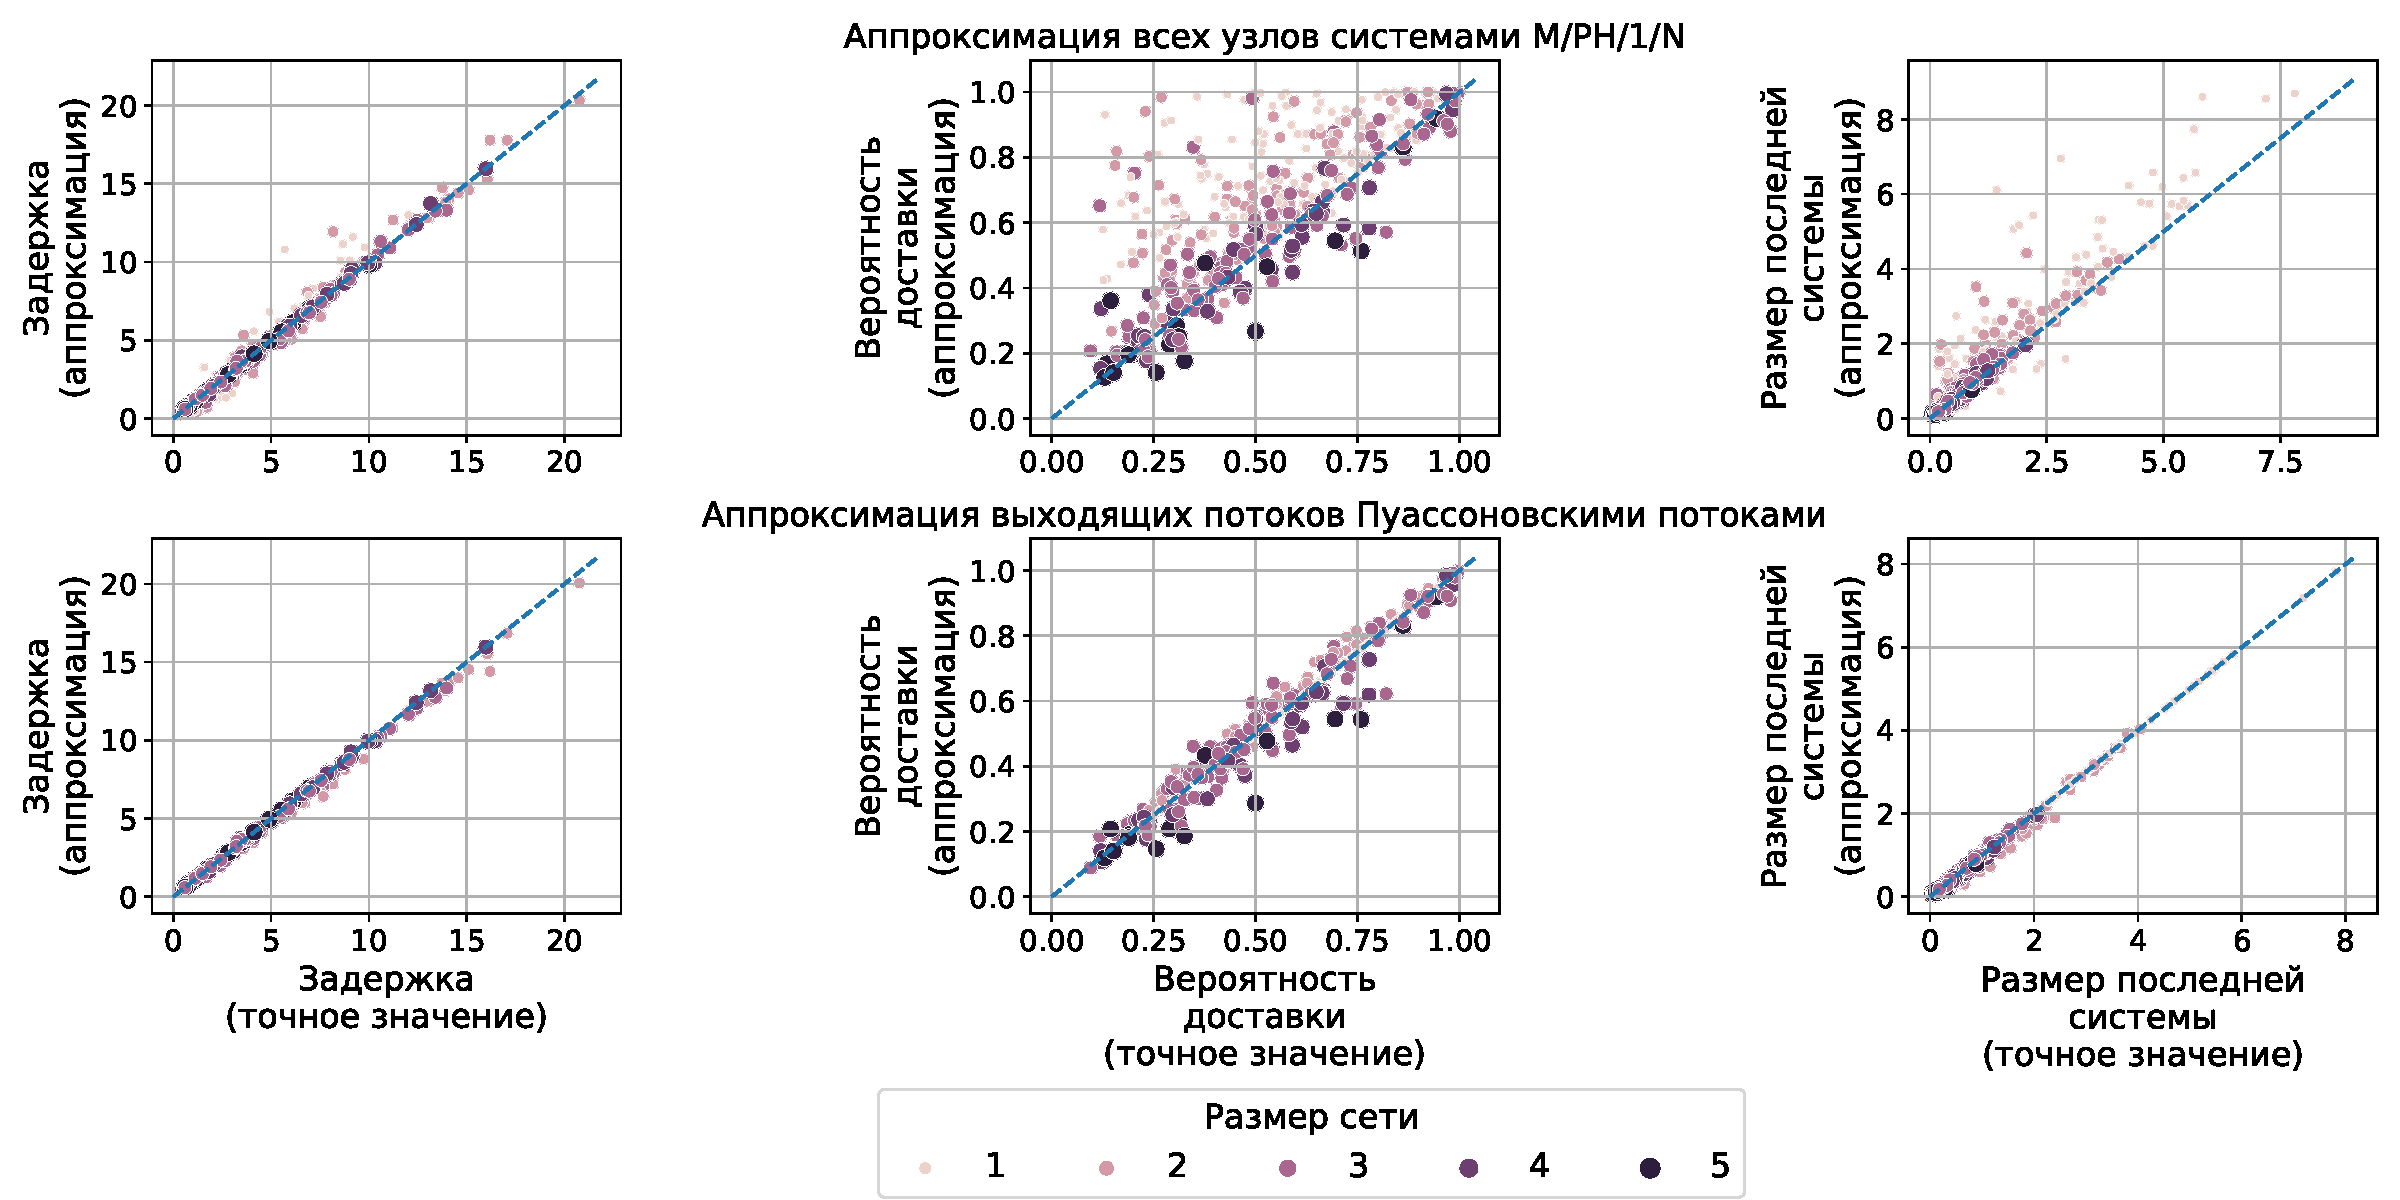
\includegraphics[width=0.8\textwidth]{chapter4/ch4_results_scatter_ph1.pdf}
  }
  \caption{Разброс оценок, полученных аппроксимацией потоков экспоненциальным распределением}
  \label{fig:ch4_results_approx_ph1}
\end{figure}

Вполне ожидаемо, аппроксимация входящего потока ведет к очень серьезным отклонениям, особенно вероятности доставки и оценки размера последней системы. В обоих случаях чаще всего получается завышенная оценка, особенно для сетей малого размера. Отметим, что разброс оценок суммарной задержки не так велик. Также отметим, что разброс оценок в случае, когда аппроксимировались только выходящие потоки, оаказался относительно небольшим.

\begin{figure}[h]
  \centerfloat{
    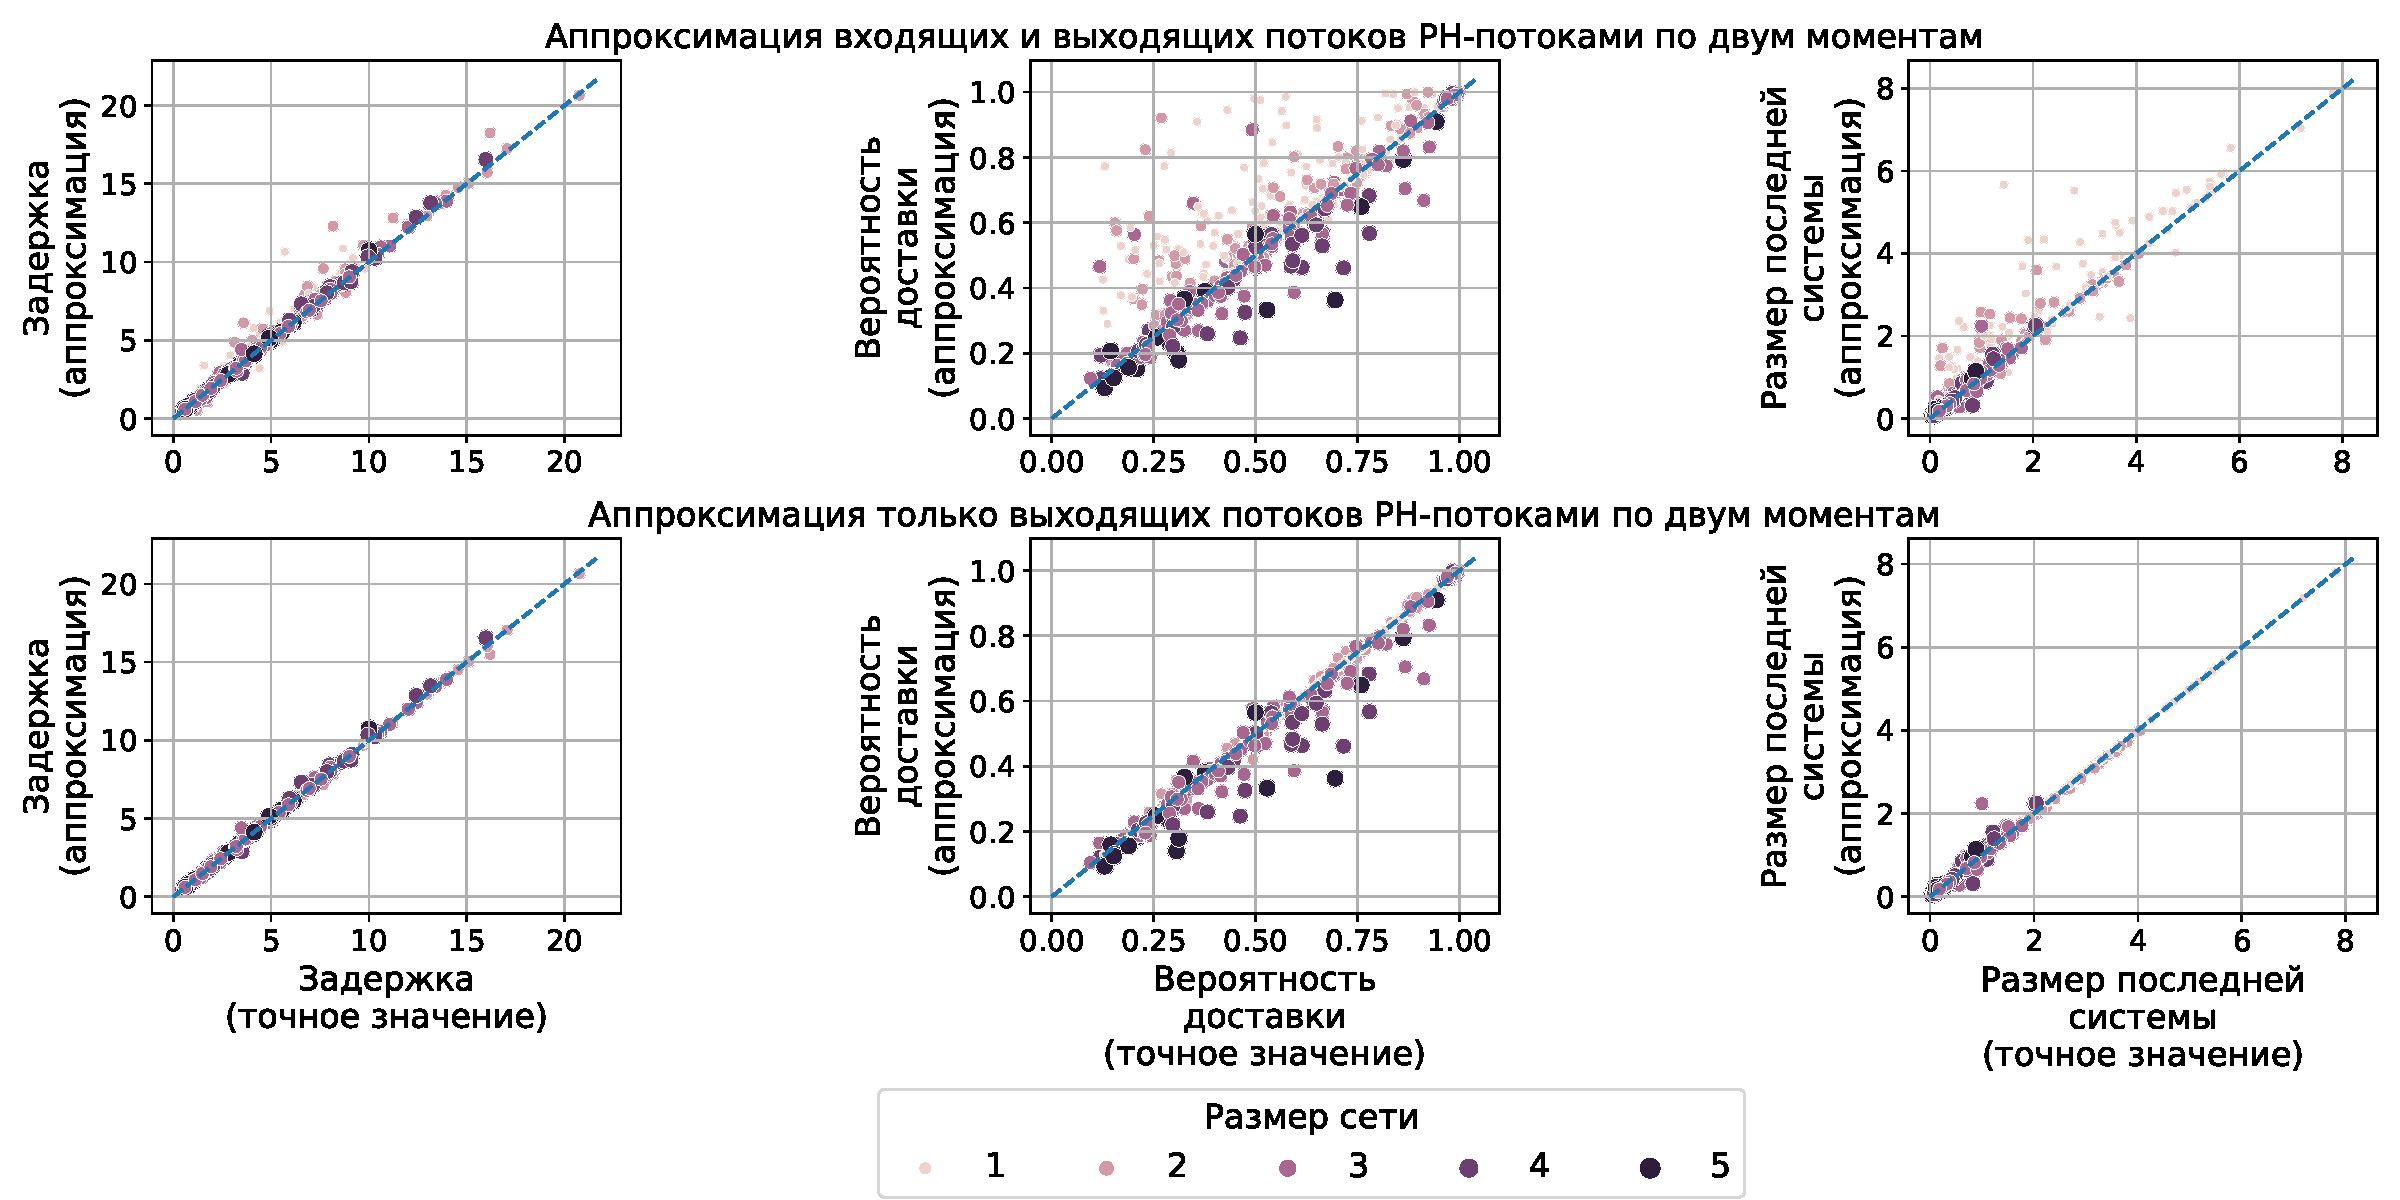
\includegraphics[width=0.8\textwidth]{chapter4/ch4_results_scatter_ph2.pdf}
  }
  \caption{Разброс оценок, полученных аппроксимацией потоков PH-распределениями по двум моментам}
  \label{fig:ch4_results_approx_ph2}
\end{figure}

Далее, было проведено сравнение с оценками, полученными аппроксимацией потоков с помощью PH-распределений по среднему и коэффициенту вариации (см. рис.~\ref{fig:ch4_results_approx_ph2}). Как и в случае с аппроксимацией потоками Пуассона, ошибки при аппроксимации входящего MAP-потока оказались существенно больше ошибок, полученных в случае аппроксимации только выходящих потоков. В то же время отметим, что разброс немного снизился по сравнению с аппроксимациями потоками Пуассона.

\begin{figure}[h]
  \centerfloat{
    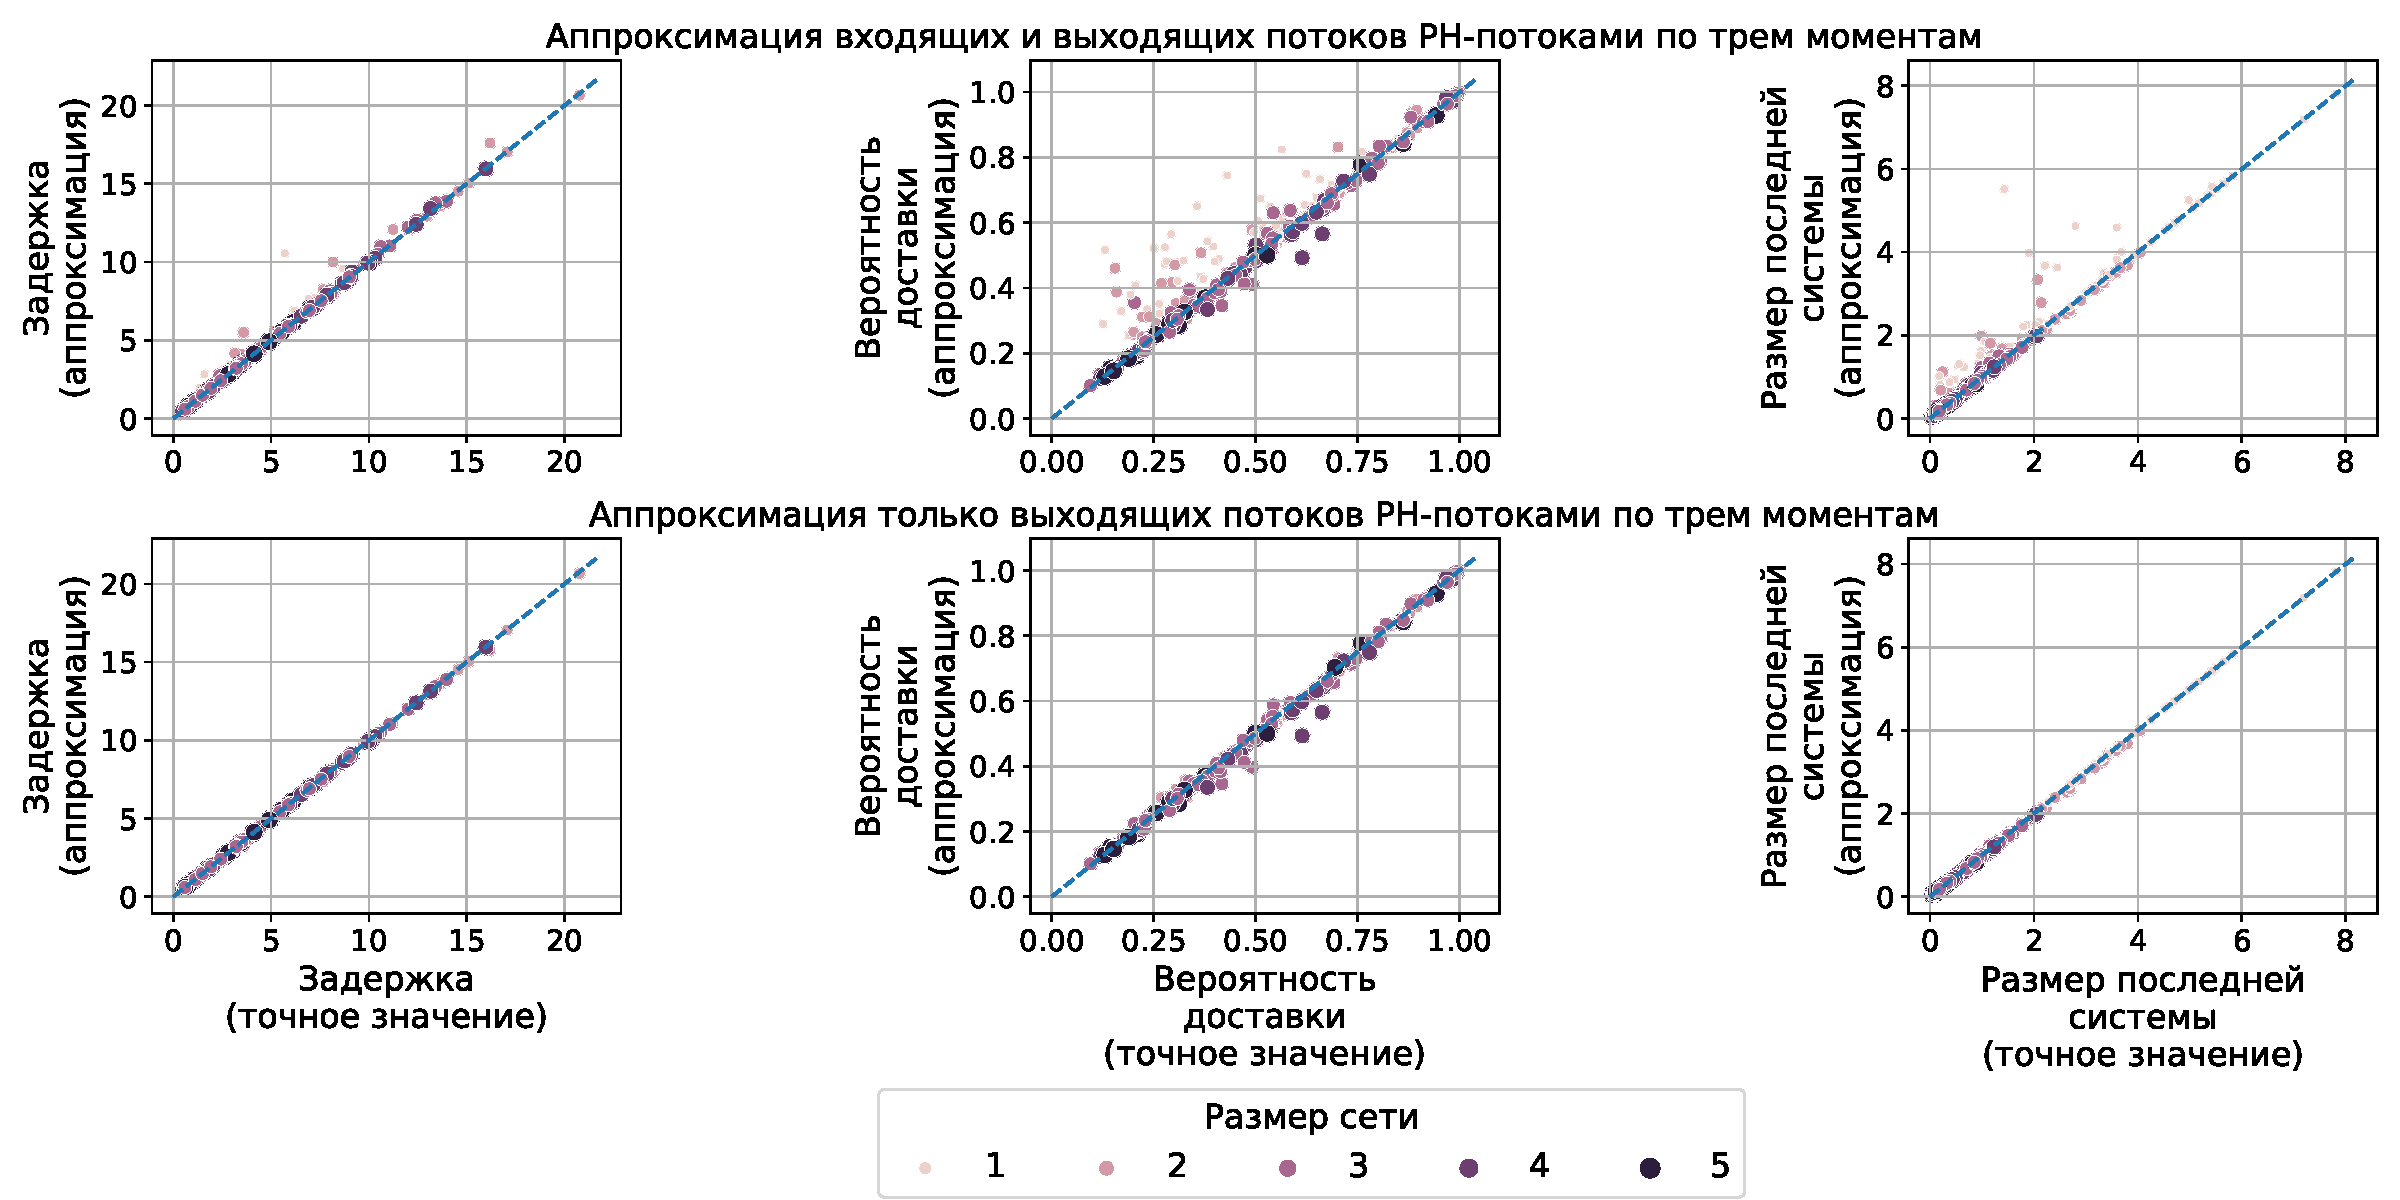
\includegraphics[width=0.8\textwidth]{chapter4/ch4_results_scatter_ph3.pdf}
  }
  \caption{Разброс оценок, полученных аппроксимацией потоков PH-распределениями по трем моментам}
  \label{fig:ch4_results_approx_ph3}
\end{figure}

На рис.~\ref{fig:ch4_results_approx_ph3} показаны результаты, полученные аппроксимацией MAP-потоков PH-распределениями по трем моментам. В этом случае, как и ранее, разброс при аппроксимации входящего потока выше разброса в случае аппроксимации только выходящих потоков, однако он существенно меньше, чем тот, что был получен предыдущими методами. Это наблюдение говорит о важности учета коэффициента асимметрии и, в то же время, о том, что отказ от учета автокорреляции входящего MAP-потока все же ведет к росту ошибок. Стоит отметить, что разброс оценок при аппроксимации только выходящих потоков очень мал.

Чтобы учесть автокорреляцию, использовался метод аппроксимации потоков новыми MAP-потоками, построенными по трем моментам и коэффициенту корреляции, который был описан в разделе~\ref{sec:ch4_approx_m3_lag1}. Разброс оценок показан на рис.~\ref{fig:ch4_results_approx_map}. Полученный разброс мало отличается как в случае аппроксимации исходного MAP-потока, так и в случае аппроксимации только выходящих MAP-потоков.

\begin{figure}[h]
  \centerfloat{
    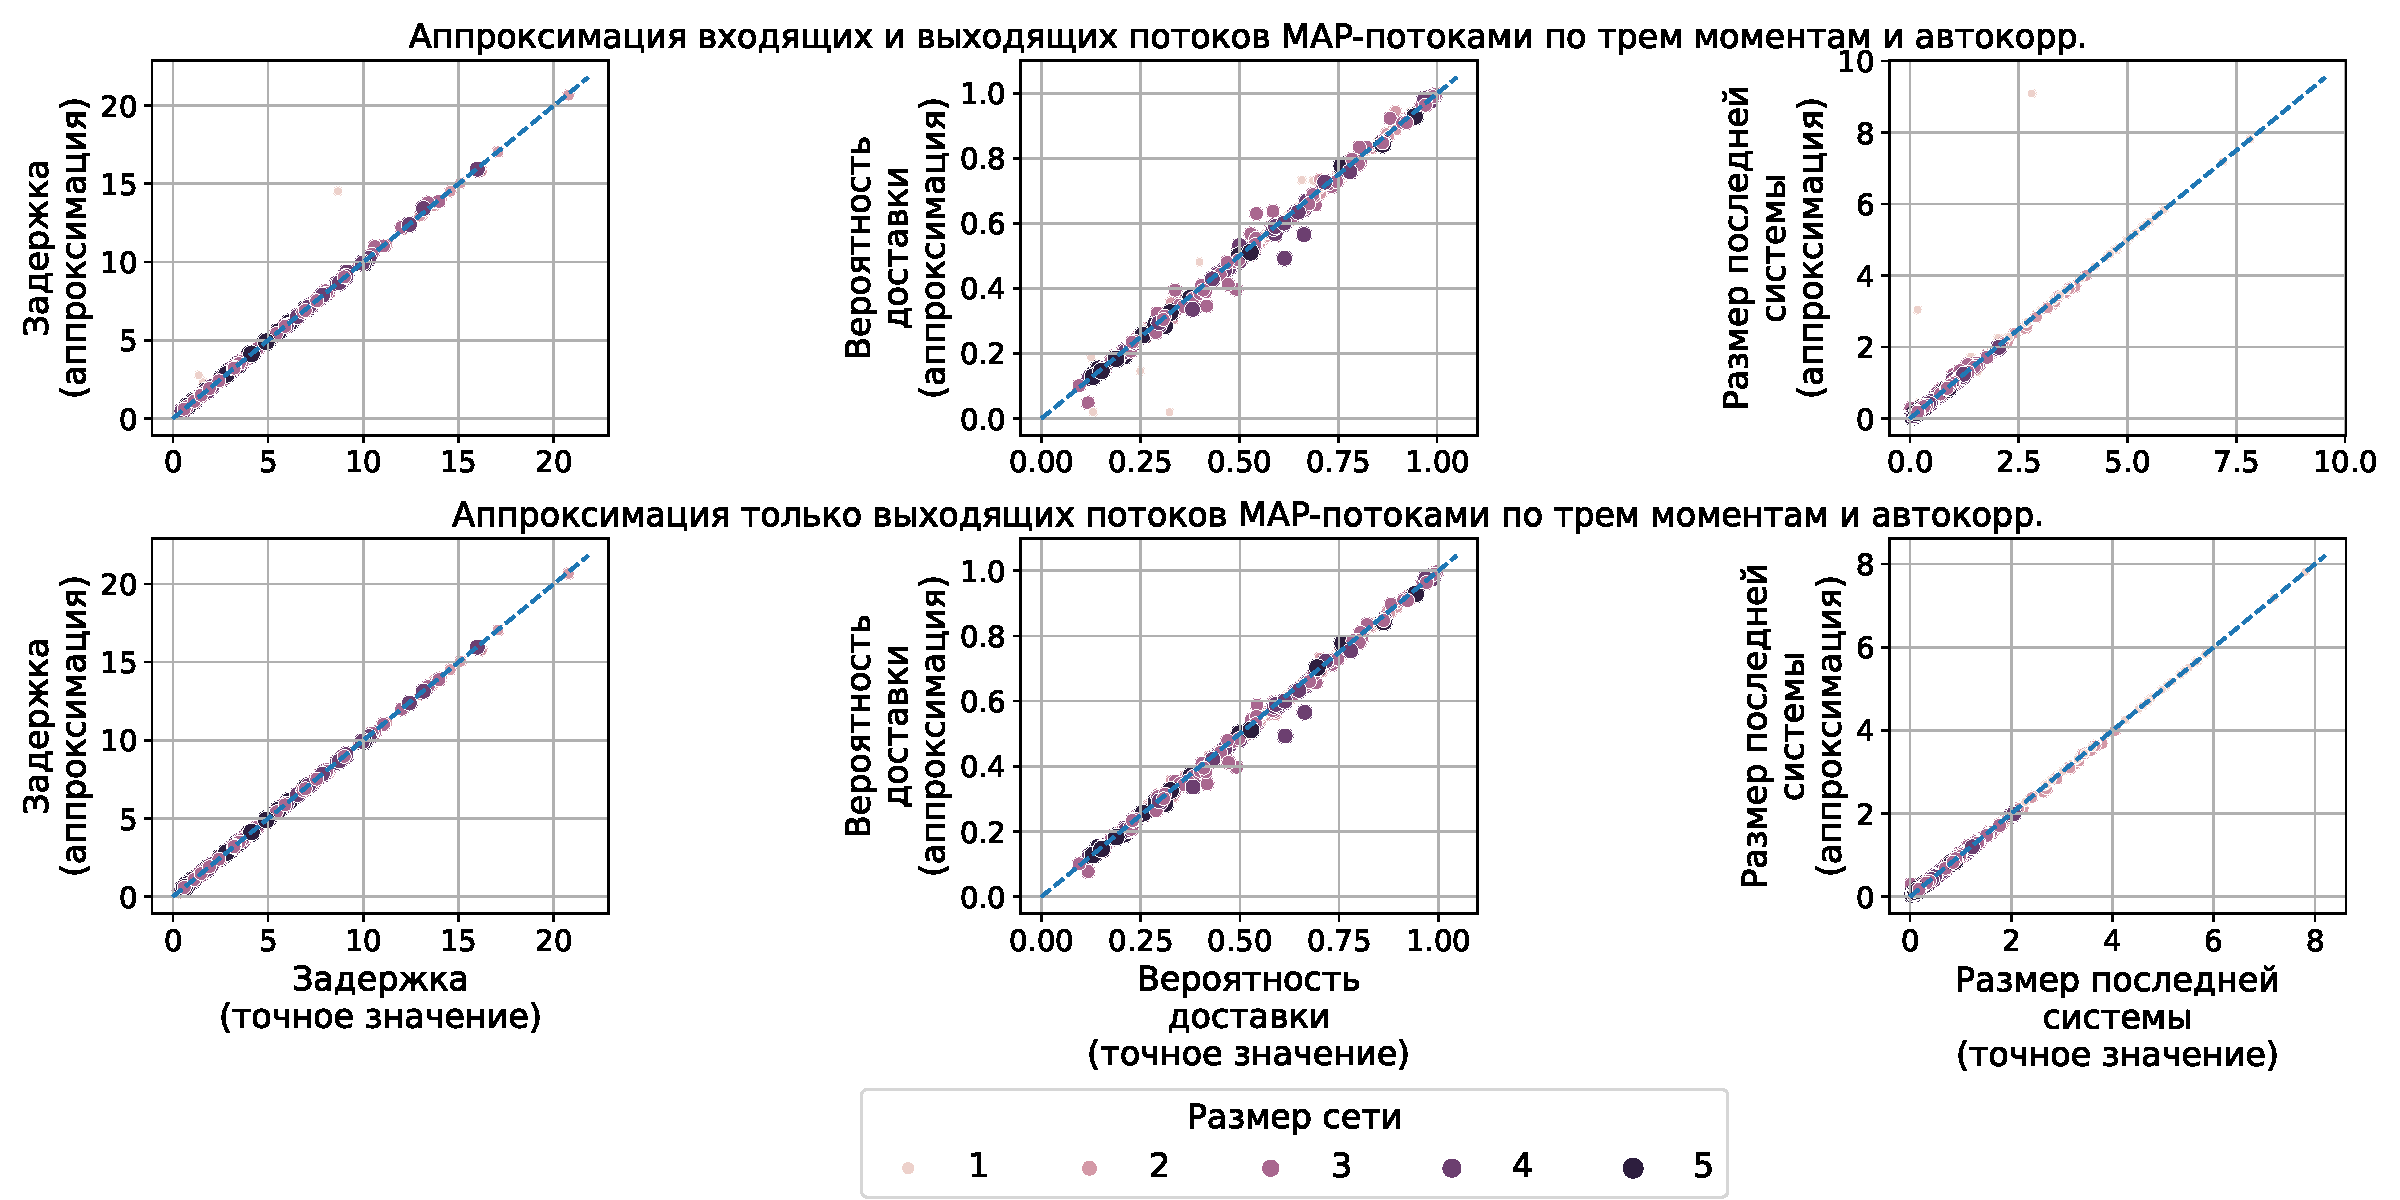
\includegraphics[width=0.95\textwidth]{chapter4/ch4_results_scatter_map.pdf}
  }
  \caption{Разброс оценок, полученных аппроксимацией MAP-потоков MAP-потоками по трем моментам и коэффициенту автокорреляции}
  \label{fig:ch4_results_approx_map}
\end{figure}

Отметим, что последний результат может быть не совсем точным, так как для генерации MAP-потоков и их аппроксимации использовались одинаковые алгоритмы. Другими словами, исходные MAP-потоки имели достаточно <<хорошую>> структуру, чтобы быть точно аппроксимируемыми. Вероятно, ошибка при аппроксимации исходных MAP-потоков может увеличиться на более реалистичных данных (например, если исходные MAP-потоки обладают значительно автокорреляцией с большими лагами или существенно иной структурой переходов в матрице $D_0$).

На рис.~\ref{fig:ch4_results_approx_mc} показан разброс оценок, полученных методом Монте-Карло. Для их получения в каждой сети моделировалось по 100 тысяч пакетов. Точность результатов оказывается наиболее высокой.

\begin{figure}[h]
  \centerfloat{
    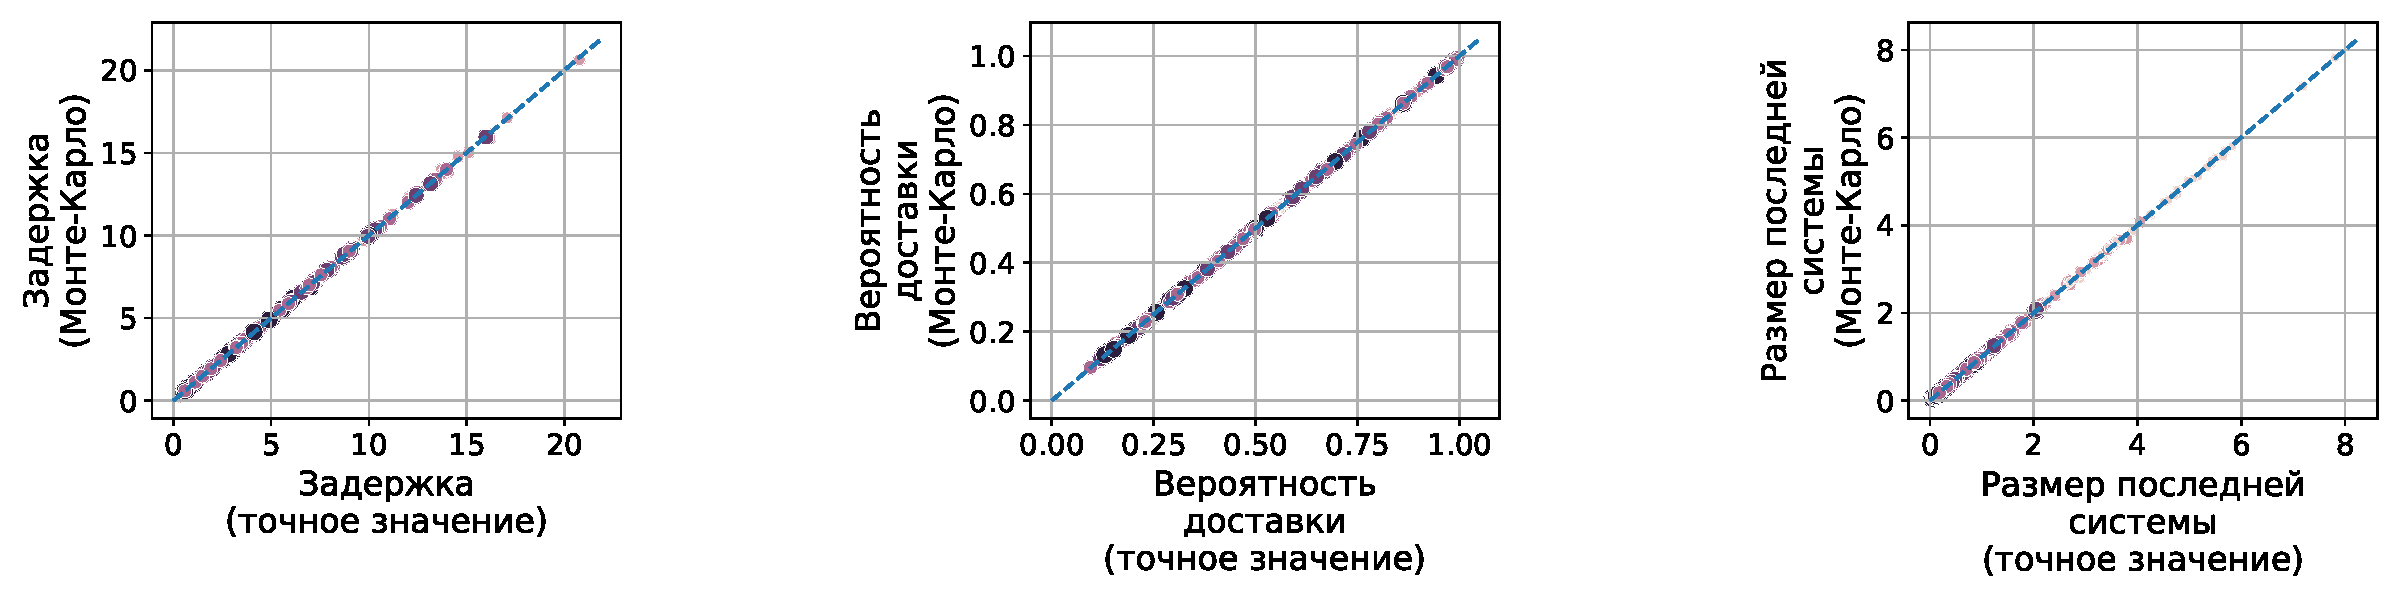
\includegraphics[width=0.95\textwidth]{chapter4/ch4_results_scatter_monte_carlo.pdf}
  }
  \caption{Разброс оценок, полученных методом Монте-Карло}
  \label{fig:ch4_results_approx_mc}
\end{figure}

Общий разброс ошибок, полученных всеми перечисленными методами, показан на рис.~\ref{fig:ch4_results_approx_summary} с помощью диаграмм типа ящики с усами. На каждом ящике с усами средняя линия соответствует медиане ($Q_2$), нижняя и верхняя границы прямоугольника "--- первый ($Q_1$) и третий ($Q_3$) квартили, а границы усов определяются, как наименьшее значение выборки, не меньшее $Q_1 - 1.5 (Q_3 - Q_1)$, и наибольшее значение, не большее $Q_3 + 1.5 (Q_3 - Q_1)$. Точки, лежащие над верхним усом "--- выбросы.

\begin{figure}[h]
    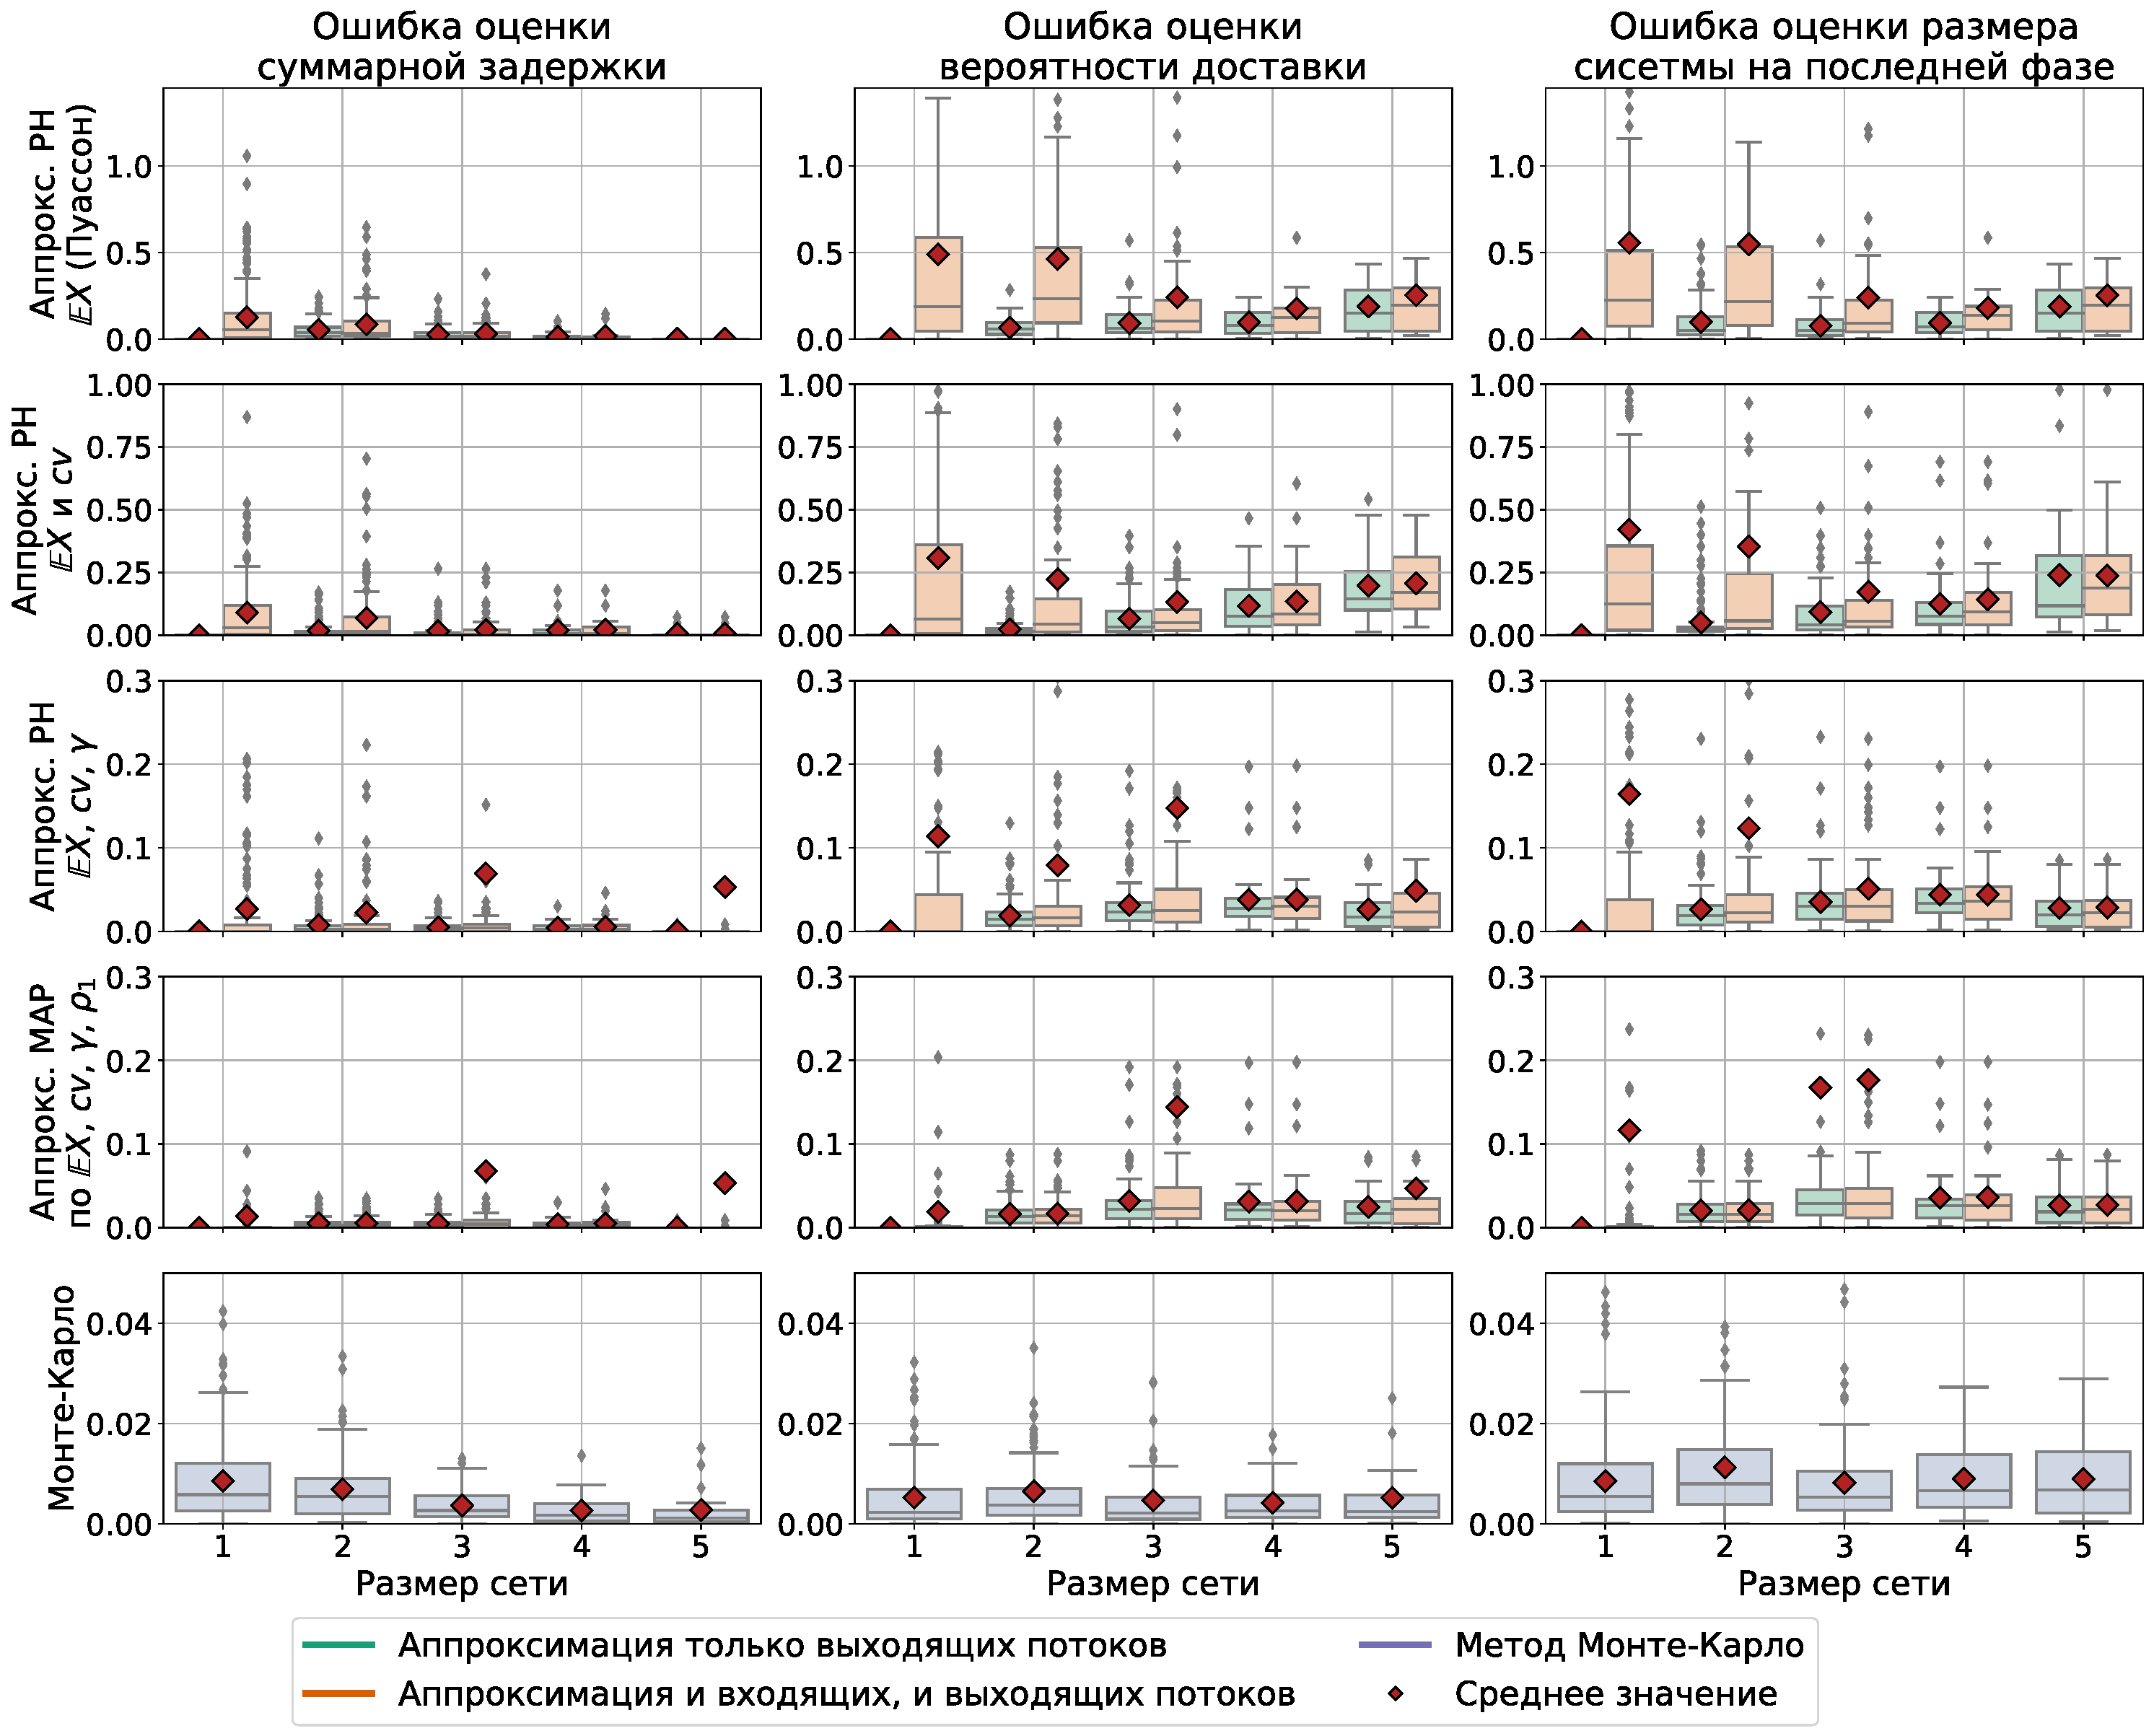
\includegraphics[width=0.95\textwidth]{chapter4/ch4_results_approx_summary.pdf}
    \legend{На каждом ящике с усами средняя линия соответствует медиане ($Q_2$), нижняя и верхняя границы прямоугольника -- первый ($Q_1$) и третий ($Q_3$) квартили, а границы усов определяются, как наименьшее значение выборки, не меньшее $Q_1 - 1.5 (Q_3 - Q_1)$, и наибольшее значение, не большее $Q_3 + 1.5 (Q_3 - Q_1)$. Точки, лежащие над верхним усом - выбросы.}
    \caption{Точность оценок, полученных с помощью методов аппроксимации потоков и метода Монте-Карло}
    \label{fig:ch4_results_approx_summary}
\end{figure}

Из приведенных на рис.~\ref{fig:ch4_results_approx_summary} данных можно сделать несколько выводов. Во-первых, ожидаемо, метод Монте-Карло дает наилучшую оценку, причем среднее не значительно выше медианы. Это говорит о том, что даже имеющиеся выбросы относительно невелики и не утягивают среднее значение вверх слишком сильно. Средняя погрешность по всем трем метрикам находится в пределах 1,5\%. Во-вторых, аппроксимация входящего MAP дает существенно большую ошибку, особенно при использовании одного или двух моментов, что подтверждает важность учета коэффициента автокорреляции. В-третьих, ошибки в оценке суммарной задержки оказались невысокими даже при аппроксимации потоками Пуассона "--- меньше 10\% в среднем для сетей длиной два и более узла. В-четвертых, вероятность доставки и средний размер последней системы удается оценить с медианной погрешностью менее 10\% при аппроксимации MAP-потоков PH-распределениями по трем моментам и, естественно, MAP-потоками по трем моментам и коэффициенту автокорреляции. В-пятых, погрешности в оценке размеров системы и вероятности доставки становятся тем меньше, чем больше узлов в сети. Наконец, в-шестых, во всех случаях при аппроксимации потоков возникают редкие выбросы, которые очень сильно повышают среднее значение. Другими словами, в подавляющем большинстве случаев удается получить оценки с небольшой погрешностью (например, около 5\% для аппроксимации PH по трем моментам), но в редких случаях ошибка аппроксимации настолько велика, что срдняя ошибка по всему множеству входных наборов достигает 20\%.

\begin{figure}[h]
  \centerfloat{
    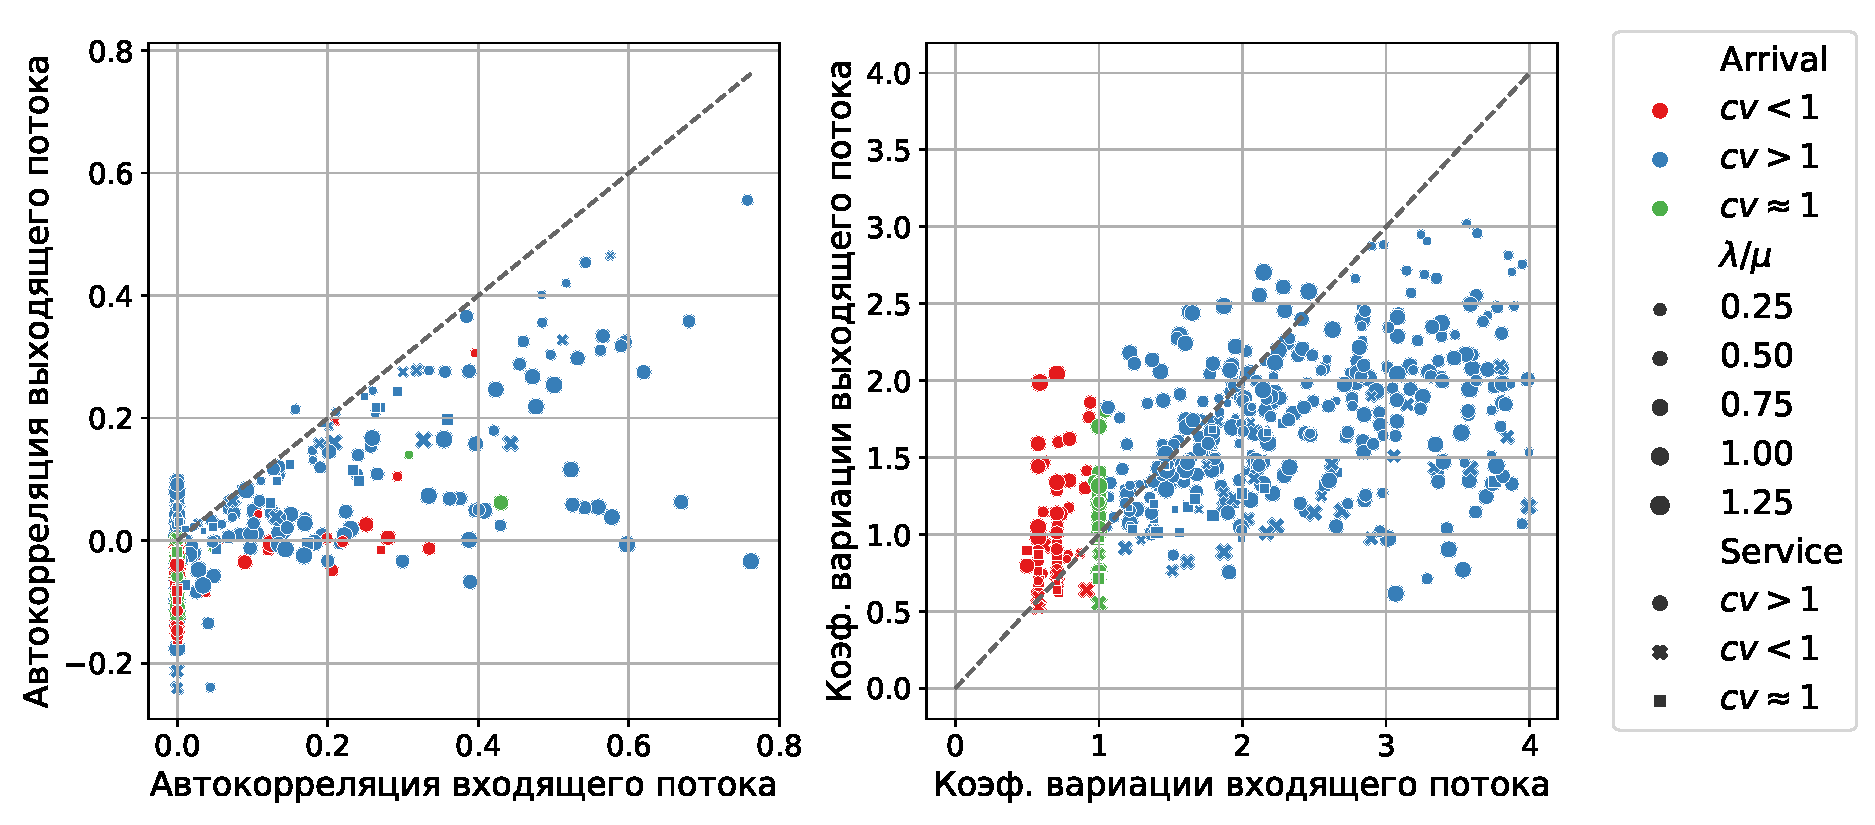
\includegraphics[width=0.95\textwidth]{chapter4/ch4_results_departure_autocorr.pdf}
  }
  \caption{Изменение коэффициентов автокорреляции и вариации в выходном потоке для системы MAP/PH/1/M}
  \label{fig:ch4_results_departure_autocorr}
\end{figure}

Рост ошибки при аппроксимации входящего MAP-потока, высокая точность Монте-Карло и улучшение приближений по мере увеличения числа аппроксимиируемых моментов были ожидаемы. В то же время, снижение ошибки при увеличении длины сети, а также практически идентичная точность при аппроксимации MAP-потоками и PH-распределениями по трем моментам, выглядят несколько неожиданно. Чтобы лучше понять причины этих наблюдений, рассмотрим, как меняется коэффициент автокорреляции и коэффициент вариации в выходном потоке. На рис.~\ref{fig:ch4_results_departure_autocorr} показан разброс коэффициентов автокорреляции и вариации во входном и выходном потоках. Во-первых, при положительной автокорреляции входящего потока, в выходящем потоке она снижается. Это правило нарушает только одно наблюдение. При нулевой автокорреляции во входящем потоке, в выходящем потоке она также снижается в большинстве случаев, хотя иногда (при высокой загрузке и положительной вариации и обслуживания, и входящего потока) может немного повыситься. Во-вторых, коэффициент вариации также меняется: если во входящем потоке вариация была больше единицы, то при относительно небольшой загрузке она уменьшается. Если же коэффициент вариации был меньше единицы (например, в случае распределений Эрланга), то вариация повышается, причем тем больше, чем выше загрузка. Такую связь с загрузкой можно объяснить тем, что когда поступления происходят чаще обслуживания (система насыщенна), на выходе наблюдается скорее распределение времени обслуживания, чем распределение интервалов между поступлениями.

\begin{figure}[h]
  \centerfloat{
    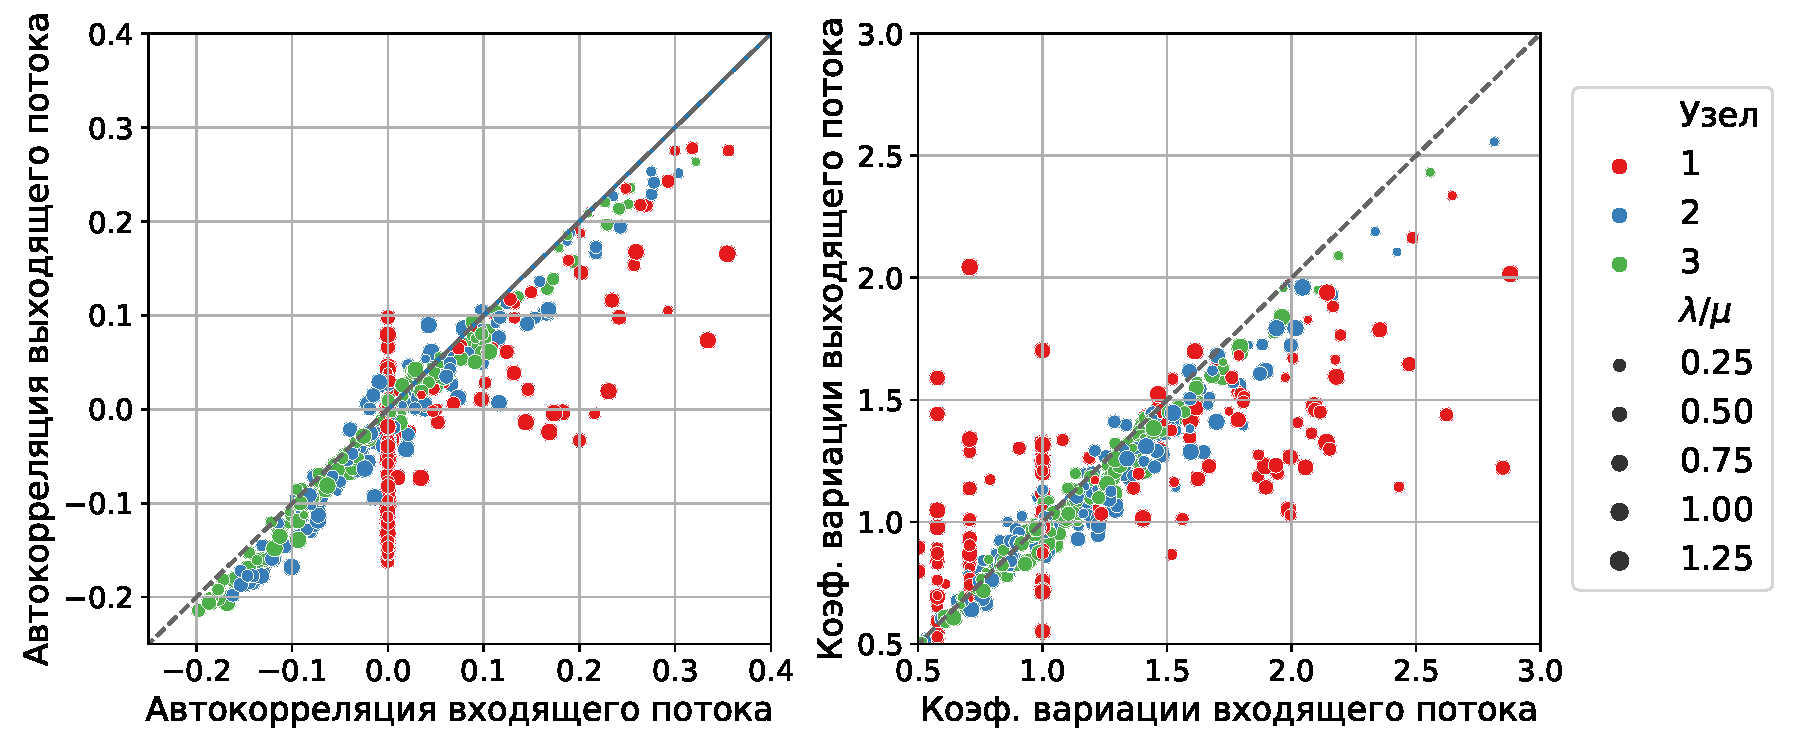
\includegraphics[width=0.95\textwidth]{chapter4/ch4_results_net_departure_autocorr.pdf}
  }
  \caption{Изменение коэффициентов автокорреляции и вариации в выходящих потоках на разных узлах сети}
  \label{fig:ch4_results_net_departure_autocorr}
\end{figure}

\begin{figure}[h]
  \centerfloat{
    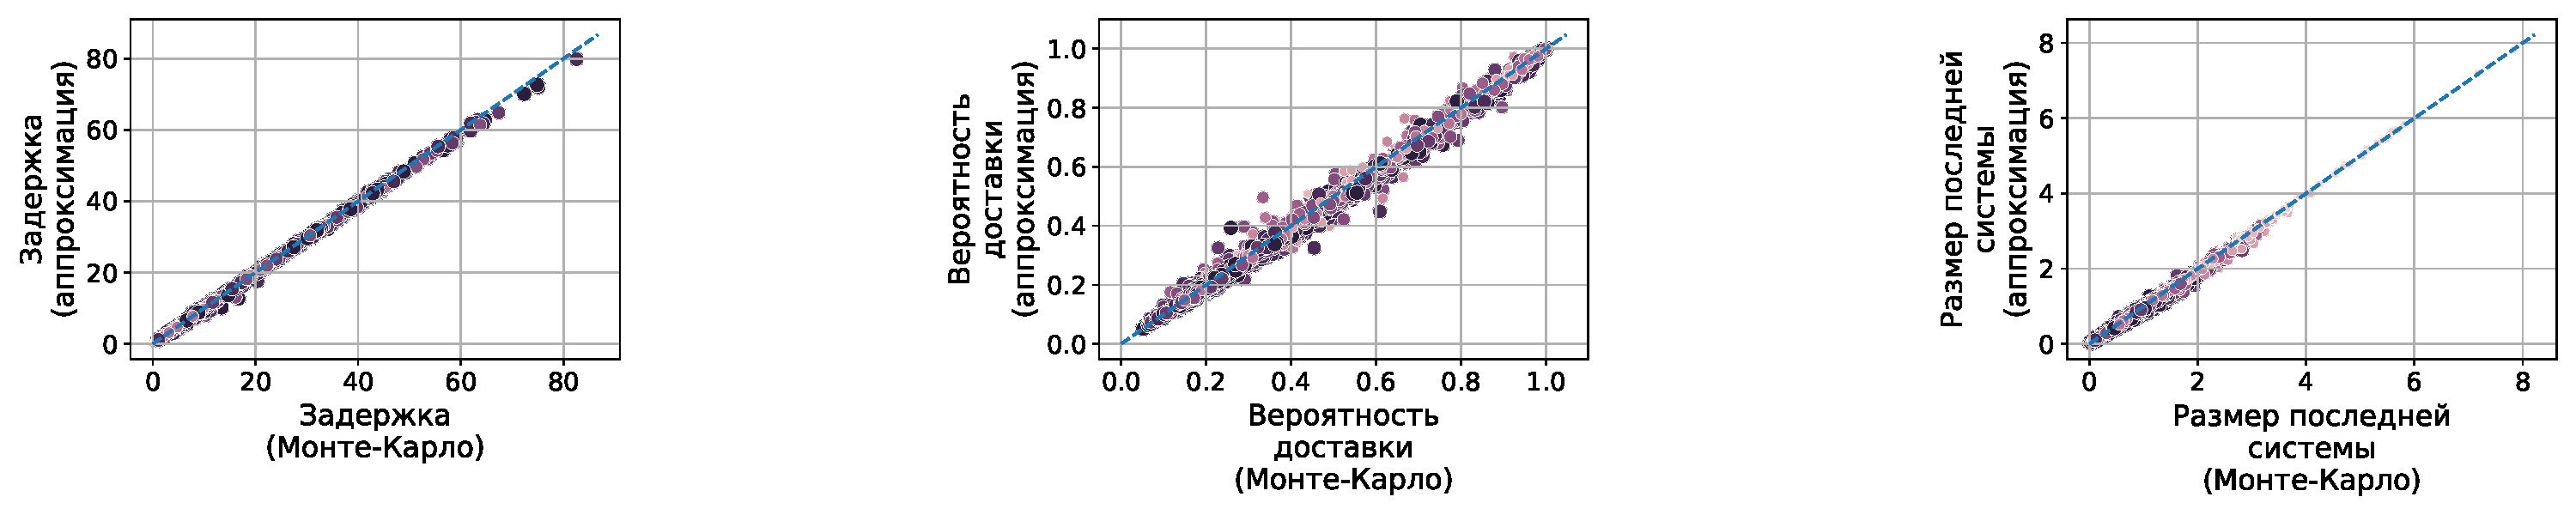
\includegraphics[width=0.95\textwidth]{chapter4/ch4_results_scatter_monte_carlo_vs_ph3.pdf}
  }
  \caption{Сравнение оценок, полученных методами Монте-Карло и аппроксимацией только выходящих потоков PH-распределениями по трем моментам}
  \label{fig:ch4_results_scatter_monte_carlo_vs_ph3}
\end{figure}

Еще более интересно отметить, что на последующих узлах сети изменения коэффициента автокорреляции и коэффициента вариации существеенно снижаются. Результаты, вычисленные для первых трех станций, показаны на рис.~\ref{fig:ch4_results_net_departure_autocorr}. Коэффициент автокорреляции также имеет тенденцию к снижению, однако его изменение становится тем меньше, чем дальше от начала сети находится узел. Коэффициент вариации также меняется тем меньше, чем дальше узел. Это позволяет понять, почему ошибки при аппроксимации выходящих потоков уменьшаются с ростом длины сети: ошибка при аппроксимации потоков на выходе с первого и второго узла может быть большой, однако далее она снижается, и общая ошибка растет медленнее по мере увеличения длины сети.

Так как наиболее точные результаты из всех методов аппроксимации были получены для аппроксимации выходящих потоков PH-распределениями по трем моментам и MAP-потоками, также была исследована точность аппроксимации относительно метода Монте-Карло. Разброс оценок для всех (и простых, и сложных) входных данных показан на рис.~\ref{fig:ch4_results_scatter_monte_carlo_vs_ph3}.

Судя по полученным результатам, аппроксимацию PH-распределениями по трем моментам можно использовать для получения приближенных оценок характеристик тандемной сети.


\subsection{Влияние коэффициента асимметрии}

Одна из особенностей, на которую стоит обратить внимание "--- существенное влияние коэффициента асимметрии при аппроксимации выходящих потоков. Погрешность, полученная при использовании аппроксимации выходящих потоков с помощью PH-распределений по двум и трем моментам, отличается более, чем в два раза (см. рис.~\ref{fig:ch4_results_approx_summary}). Для более глубокого понимания зависимостей были проведены расчеты задержек и вероятностей успешной доставки в зависимости от коэффициентов асимметрии входящего потока (см. рис.~\ref{fig:ch4_results_arrival_skewness}) и распределения времени обслуживания (см. рис.~\ref{fig:ch4_results_service_skewness}) при различных коэффициентах вариации.

\begin{figure}[h]
  \centerfloat{
    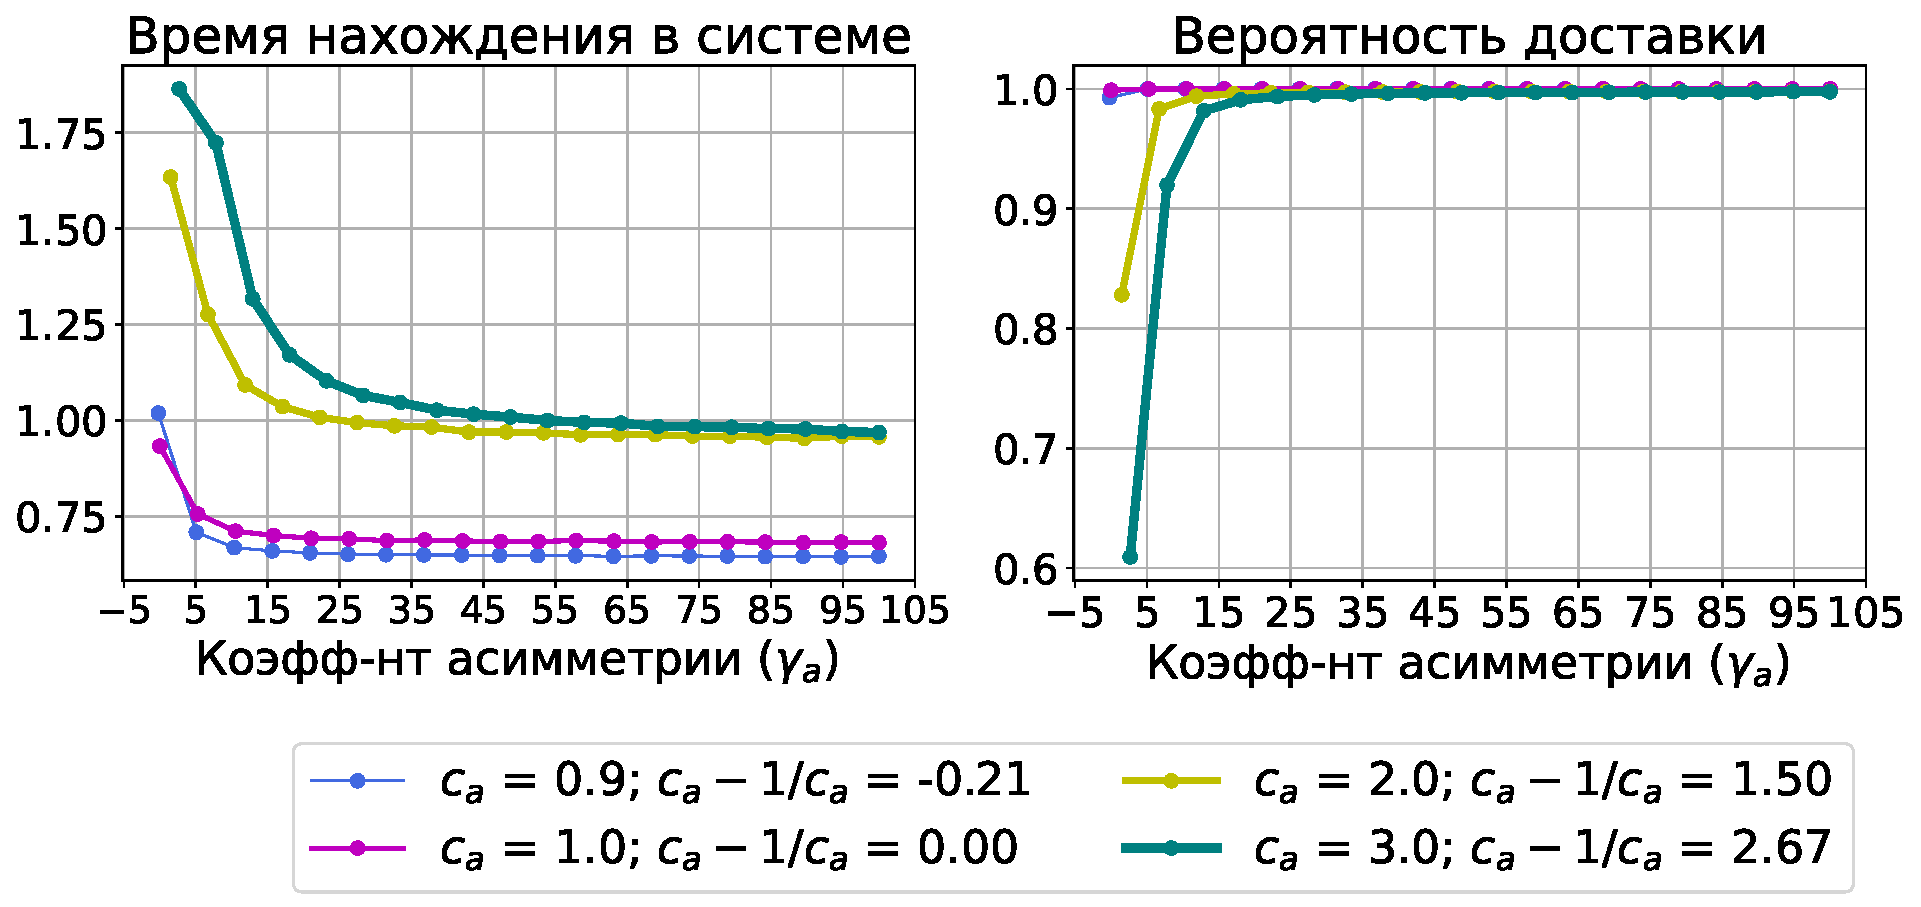
\includegraphics[width=0.8\textwidth]{chapter4/ch4_results_arrival_skewness.pdf}
  }
  \caption{Влияние коэффициента асимметрии входящего потока на задержку и вероятность доставки в системе MAP/PH/1/M}
  \label{fig:ch4_results_arrival_skewness}
\end{figure}

В этих экспериментах рассматривался один узел MAP/PH/1/M с коэффициентом загрузки 0,5 ($m_a = 1, m_s = 0,5$) и емкостью очереди $M = 6$. Для исследуемого распределения (интервалов во входящем потоке или времени обслуживания) рассматривались четыре значения коэффициента вариации $c_{a,s} = \{0,9; 1; 2; 3\}$, а для другого распределения (соответственно, времени обслуживания и интервалов во входящем потоке) коэффициент полагался равным $c_{s,a} = 0,9$. Коэффициент асимметрии для исследуемого распределения менялся в интервале $[c_{a,s} - 1/c_{a,s}, 100]$, а для зафиксированного полагался равным $c_{s,a} - 1/c_{s,a} = -19/90$.

\begin{figure}[h]
  \centerfloat{
    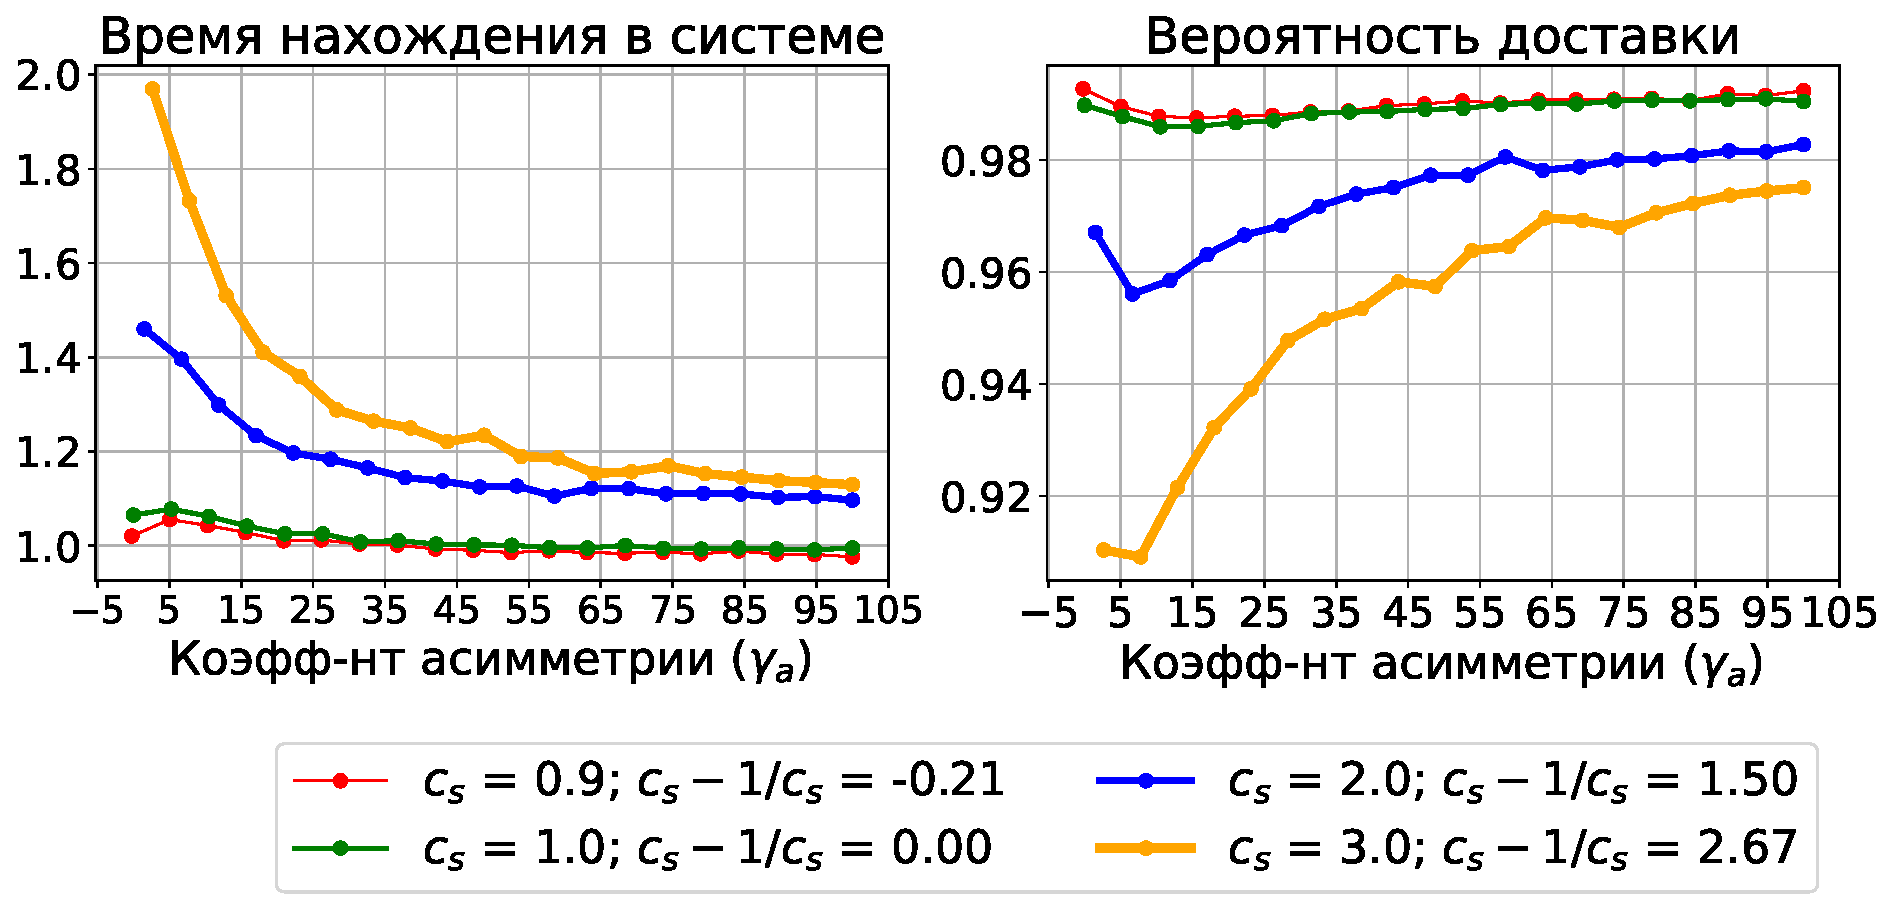
\includegraphics[width=0.8\textwidth]{chapter4/ch4_results_service_skewness.pdf}
  }
  \caption{Влияние коэффициента асимметрии распределения времени обслуживания на задержку и вероятность доставки в системе MAP/PH/1/M}
  \label{fig:ch4_results_service_skewness}
\end{figure}

Из приведенных результатов можно сделать несколько выводов. Во-первых, коэффициент асиммтерии входящего потока сильно влияет на характеристики системы, причем влияние тем сильнее, чем выше коэффициент вариации, а для $c_a > 1$ нужно учитывать конкретные значения $\gamma_a$ даже при $\gamma_a \gg 1$ (см. кривые на рис.~\ref{fig:ch4_results_arrival_skewness} при $c_a = 2,0, 3,0$). Во-вторых, коэффициент асиммтерии времени обслуживания также оказывает влияние, но меньшее, и при росте $\gamma_s$ больше некоторого значения $\underline{\gamma_s} = \underline{\gamma_s}(c_s)$, зависящего от коэффициента варации $c_s$, это влияние практически пропадает. В рассмотренном случае можно приблизительно оценить эти значения как $\underline{\gamma_s}(1) = \underline{\gamma_s}(0.9) \approx 15$, $\underline{\gamma_s}(2) \approx 25$ и $\underline{\gamma_s}(3) \approx 55$ (см. рис.~\ref{fig:ch4_results_service_skewness}). Таким образом, чем больше вариация, тем больший диапазон асимметрии надо учитывать.

Если коэффициент асимметрии входящего потока существенно влияет и на задержку, и на вероятность доставки, то коэффициент асимметрии времени обслуживания влияет существенно сильнее на вероятность доставки, чем на задержку. Так, в исследуемом случае задержка практически не меняется для любых $\gamma_s > 15$. В то же время, при небольших значениях $\gamma_s < 15$ влияние на задержку также достаточно сильное, причем тем больше, чем выше коэффициент вариации $c_s$. Отметим, что конкретные виды зависимости могут отличаться в зависимости от коэффициента загрузки $m_s / m_a$, емкости очереди $M$ и коэффициентов автокорреляции.

Из приведенных численных результатов можно сделать вывод, что при аппроксимациях выходящих потоков, а также при поиске подходящего распределения времени обслуживания (например, если требуется описать время передачи пакетов в канале связи) важно учитывать коэффициент асимметрии. В частности, будем далее руководствоваться этим результатом при построении моделей каналов беспроводных сетей.


\subsubsection{Скорость вычислений и сходимость метода Монте-Карло}

Для всех методов аппроксимации, точного решения и метода Монте-Карло были проведены измерения времени, необходимого для получения оценок, результаты показаны на рис.~\ref{fig:ch4_results_approx_elapsed}.

Из рис.~\ref{fig:ch4_results_approx_elapsed} можно отметить следующее. Во-первых, точное решение требует больше всего времени. Это связано с необходимостью обращать матрицы и решать системы линейных уравнений очень высокого порядка (размеры матриц были ограничены 8000-ми строк/столбцов). Во-вторых, аппроксимация MAP-потоками также работает долго. Причина "--- необходимость решать задачу оптимиазации для поиска элементов матрицы $D_1$ (поиск минимума и максимума допустимых коэффициентов автокорреляции для заданной матрицы $D_0$). В-третьих, остальные методы аппроксимации работают быстрее метода Монте-Карло. Так, если для сетей с 9 узлами метод Монте-Карло требует порядка 200--300~мс., то аппроксимация PH-распределениями по трем моментам -- около 150~мс., а аппроксимация PH-распределениями по одному или двум моментам -- менее 50~мс. Отметим, что все численные эксперименты проиводились на рабочей станции с процессором Intel Core i7-9700K под управлением ОС Ubuntu Linux. Код имитационной модели компилировался с помощью компилятора GCC с уровнем оптимизации O3. Расчет методом аппроксимации потоков был реализован на Python с использованием библиотек NumPy и SciPy.

\begin{figure}[h]
  \centerfloat{
    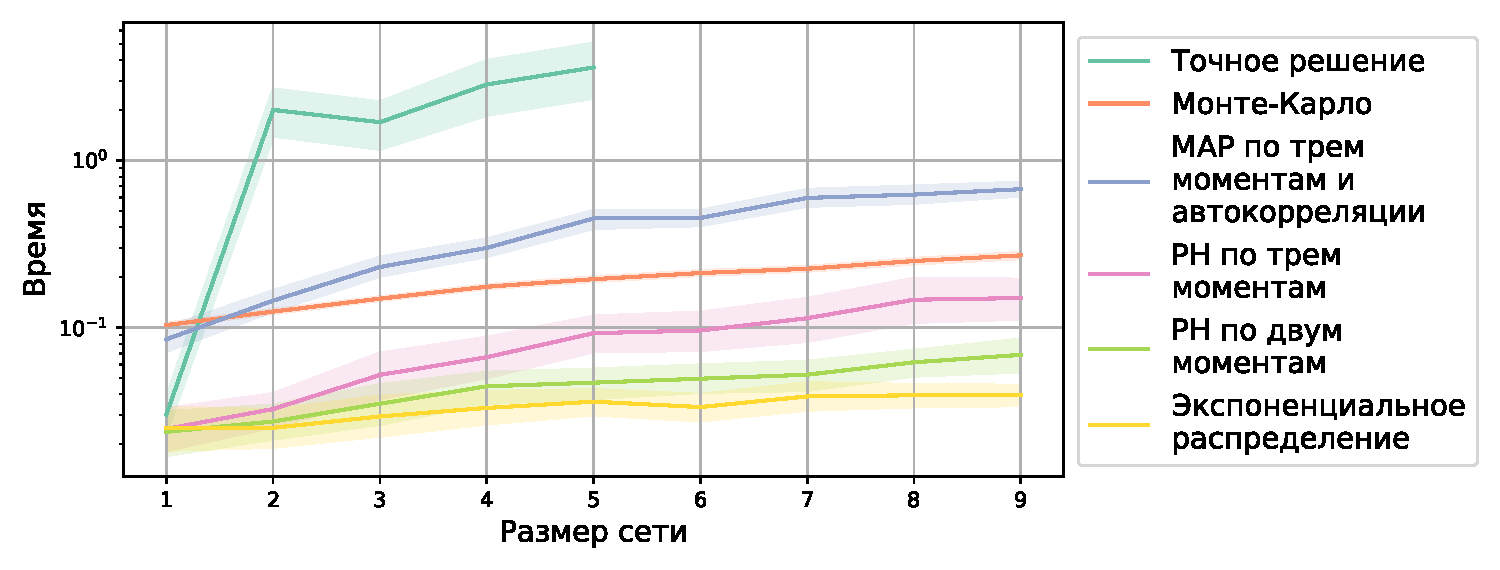
\includegraphics[width=0.95\textwidth]{chapter4/ch4_results_approx_elapsed.pdf}
  }
  \caption{Длительность расчета точного решения, а также расчетов с помощью различных методов аппроксимации выходящих потоков и метода Монте-Карло}
  \label{fig:ch4_results_approx_elapsed}
\end{figure}

Наконец, отметим, что 100 тыс. пакетов для метода Монте-Карло является даже избыточным. На рис.~\ref{fig:ch4_results_monte_carlo_performance} показано, как меняется точность результатов от числа промоделированных пакетов, а также то, как меняется время, расходуемое на выполнение метода. Так, для получения точности 5~\% оказывается достаточно промоделировать около 50 тыс. пакетов. Ограничить число пакетов представляется разумным в свете того, что необходимое время зависит от числа пакетов почти линейно.

\begin{figure}[h]
  \centerfloat{
    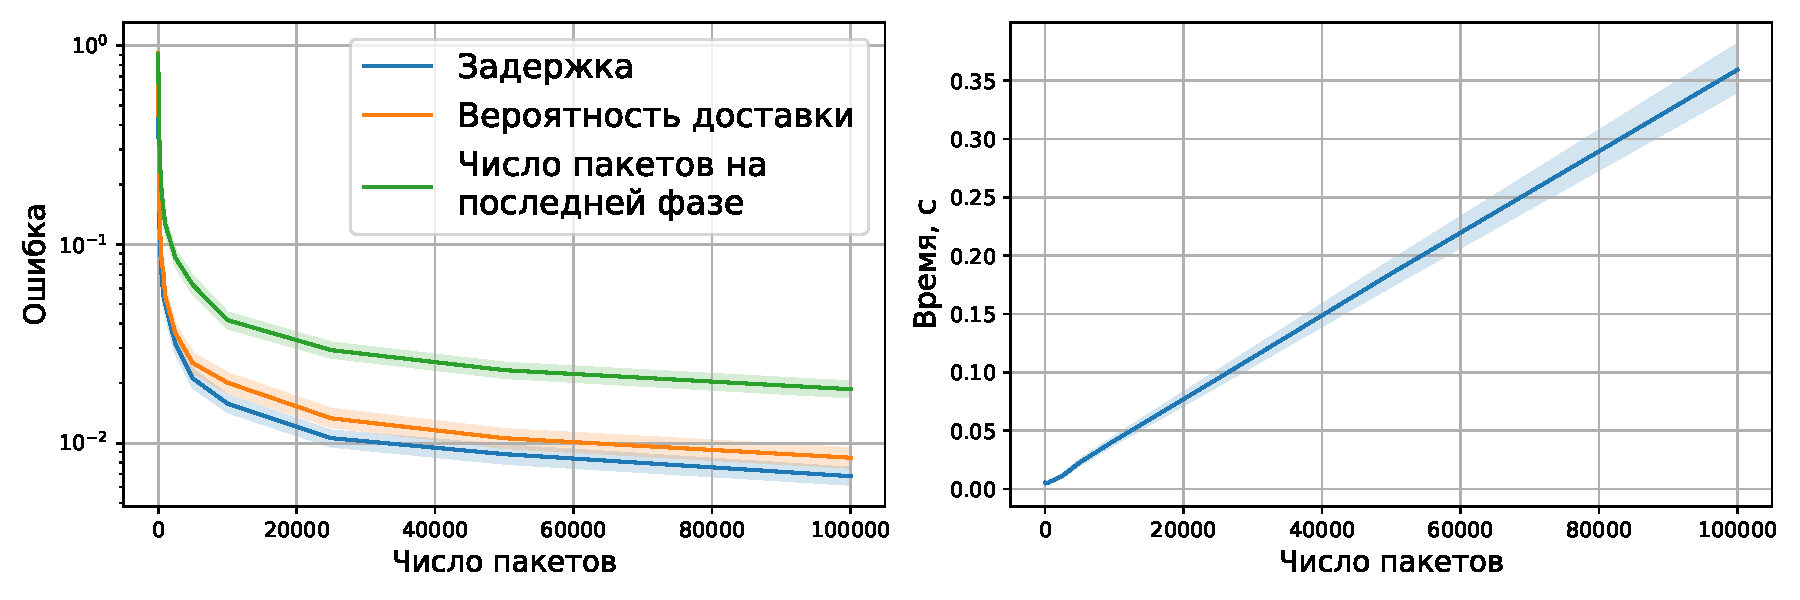
\includegraphics[width=0.95\textwidth]{chapter4/ch4_results_monte_carlo_performance.pdf}
  }
  \caption{Сходимость метода Монте-Карло и скорость выполнения расчетов}
  \label{fig:ch4_results_monte_carlo_performance}
\end{figure}
























%%%%%%%%%%%%%%%%%%%%%%%%%%%%%%%%%%%%%%%%%%%%%%%%%%%%%%%%%%%%%%%%%%%%%%%%%%%%%%%%
\section{Численный расчёт характеристик многошаговой беспроводной сети}\label{sec:ch4_results_networks}
%%%%%%%%%%%%%%%%%%%%%%%%%%%%%%%%%%%%%%%%%%%%%%%%%%%%%%%%%%%%%%%%%%%%%%%%%%%%%%%%

В численном эксперименте были исследованы характеристики многошаговых беспроводных сетей с помощью метода, описанного в разделе~\ref{sec:ch4_wireless_network_model}. Предполагалось, что сеть работает в ad-hoc режиме по стандарту IEEE 802.11 DCF без RTS/CTS. Параметры настройки протокола приведены в табл.~\ref{table:ch4_channel_parameters}. Беспроводная сеть моделировалась в системе моделирования NS-3, в каждом запуске моделировалась передача 500'000 пакетов.

\begin{table}[h!]\centering{
\begin{tabular}{|c|c|c|c|}\hline
Параметр & Значение & Единицы\\ \hline
Заголовок PHY & 128 & бит\\
Заголовок MAC DATA & 208 & бит \\
Кадр MAC ACK & 96 & бит \\
Слот ($\sigma$) & 9 & мкс \\
DIFS & 34 & мкс\\
SIFS & 16 & мкс \\
CWmin & 16 & - \\
CWmax & 1024 & - \\
Скорость канала & 54 & мегабит/с \\
Заголовок IP & 160 & бит \\ \hline
Средний размер пакета данных ($\overline{\xi}$) & 11200 & бит\\
Минимальная интенсивность трафика ($B_\text{min}$) & 1,2 & мегабит/с \\
Максимальная интенсивность трафика ($B_\text{max}$) & 12 & мегабит/с \\ \hline
\end{tabular}\caption{Параметры беспроводных каналов и трафика для эксперимента}\label{table:ch4_channel_parameters}
}\end{table}

Входящий трафик моделировался пуассоновскими потоками с четырьмя интенсивностями $\lambda = 100, 200, 500, 1000$. Учитывая, что средний размер пакетов, поступающих от пользователей, был равен 11200~бит, эти потоки соответствовали трафику 1,2, 2,4, 6 и 12 мегабит в секунду.

Для получения PH-распределений, моделирующих время передачи пакетов в каналах, с помощью имитационной модели беспроводной сети в NS-3 была собрана статистика длительностей передачи пакетов в каждом из четырех каналов, показанных на рис.~\ref{fig:ch4_channel_model_schema}. Далее, для каждого канала по трем моментам было найдено PH-распределение с помощью метода, описанного в разделе~\ref{sec:ch4_approx_m3}. Сравнение эмпирических распределений длительностей передачи, полученных из имитационной модели, и найденных PH-распределений, показано на рис.~\ref{fig:ch4_results_networks_channel_dist}.

\begin{figure}[h]
  \centerfloat{
    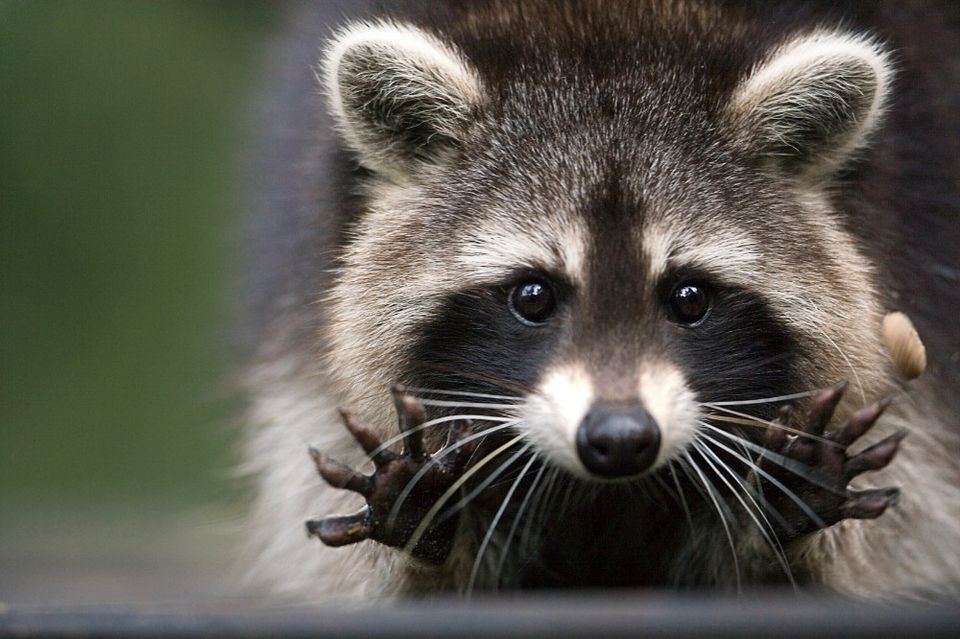
\includegraphics[width=0.7\textwidth]{chapter4/raccoon-1.jpg}
  }
  \caption{Сравнение распределений длительностей передачи пакетов в каналах, полученных из имитационной модели, и моделирующих PH-распределений}
  \label{fig:ch4_results_networks_channel_dist}
\end{figure}

Для получения оценок длительности передачи пакетов в сети с помощью модели сети массового обслуживания MAP/PH/1/N $\rightarrow \bullet$/PH/1/N $\rightarrow \dots \rightarrow \bullet$/PH/1/N, содержащей больше пяти станций, промежуточные каналы моделировались тем же PH-распределением, что и канал $S_2 \rightarrow S_3$ (см. рис.~\ref{fig:ch4_network_model}). Для более высокой точности, характеристики модели сети массового обслуживания были получены с помощью метода Монте-Карло, хотя, как было показано ранее, для этой цели можно было бы использовать также метод аппроксимации выходящих потоков.
% Сравнение результатов приведено на рис.~\ref{xxx}.



%%%%%%%%%%%%%%%%%%%%%%%%%%%%%%%%%%%%%%%%%%%%%%%%%%%%%%%%%%%%%%%%%%%%%%%%%%%%%%%%
\section{Заключение}\label{sec:ch4_conclusion}
%%%%%%%%%%%%%%%%%%%%%%%%%%%%%%%%%%%%%%%%%%%%%%%%%%%%%%%%%%%%%%%%%%%%%%%%%%%%%%%%
В главе были представлены следующие результаты.

\begin{enumerate}
  \item Предложена методика нахождения PH-распределений для моделирования задержек в каналах многошаговых беспроводных сетей, учитывающая интерференцию между соседними станциями.
  \item Предложен метод нахождения приближенных значений характеристик открытых сетей массового обслуживания с узлами MAP/PH/1/N с помощью аппроксимации потоков обслуженных пакетов.
  \item Представлены результаты имитационного моделирования многошаговых беспроводных сетей IEEE 802.11 и сетей с радиорелейными каналами и проведено численное сравнение с результатами, полученными с помощью моделей сетей массового обслуживания с узлами MAP/PH/1/N. Показано, что при средней интенсивности трафика модели сетей массового обслуживания дают результаты, близкие к результатам имитационного моделирования беспроводных сетей. Также показано, что метод аппроксимации выходящих потоков позволяет получить достаточно точные результаты, используя значительно меньше вычислительных ресурсов.
  \item Показано, что при моделировании радиорелейных сетей выходящие потоки следует аппроксимировать MAP-потоками порядка выше единицы. Однако, при моделировании сетей с каналами IEEE 802.11 DCF можно аппроксимировать выходящие потоки MAP-потоками первого порядка, то есть простейшими потоками Пуассона.
  \item Представлены результаты имитационного и стендового моделирования многошаговой беспроводной сети с каналами IEEE 802.11g, показывающие, что такую сеть можно успешно использовать для передачи данных с большого количества RFID-считывателей (порядка нескольких сот считывателей).
\end{enumerate}


\clearpage
